%%%%%%%%%%%%%%%%%%%%%%%%%%%%%%%%%%%%%%%%%
% Academic Title Page
% LaTeX Template
% Version 2.0 (17/7/17)
%
% This template was downloaded from:
% http://www.LaTeXTemplates.com
%
% Original author:
% WikiBooks (LaTeX - Title Creation) with modifications by:
% Vel (vel@latextemplates.com)
%
% License:
% CC BY-NC-SA 3.0 (http://creativecommons.org/licenses/by-nc-sa/3.0/)
% 
% Instructions for using this template:
% This title page is capable of being compiled as is. This is not useful for 
% including it in another document. To do this, you have two options: 
%
% 1) Copy/paste everything between \begin{document} and \end{document} 
% starting at \begin{titlepage} and paste this into another LaTeX file where you 
% want your title page.
% OR
% 2) Remove everything outside the \begin{titlepage} and \end{titlepage}, rename
% this file and move it to the same directory as the LaTeX file you wish to add it to. 
% Then add \input{./<new filename>.tex} to your LaTeX file where you want your
% title page.
%
%%%%%%%%%%%%%%%%%%%%%%%%%%%%%%%%%%%%%%%%%

%----------------------------------------------------------------------------------------
%	PACKAGES AND OTHER DOCUMENT CONFIGURATIONS
%----------------------------------------------------------------------------------------

\documentclass[12pt]{scrartcl}

\usepackage[utf8]{inputenc} % Required for inputting international characters
\usepackage[T1]{fontenc} % Output font encoding for international characters
\usepackage{lmodern}
%\usepackage{mathpazo} % Palatino font

\usepackage{graphicx}
\usepackage{wrapfig}
\usepackage[dvipsnames]{xcolor}
\usepackage{multicol}
\usepackage{caption}
\usepackage{colortbl}

\usepackage{enumitem}

\usepackage{tikz}
\usetikzlibrary{trees, calc, arrows, automata}
\def\tick{{\color{green}\tikz\fill[scale=0.4](0,.35) -- (.25,0) -- (1,.7) -- (.25,.15) -- cycle;}} 
\def\scalecheck{\resizebox{\widthof{\checkmark}*\ratio{\widthof{x}}{\widthof{\normalsize x}}}{!}{\checkmark}}

\usepackage{amsmath}
\usepackage{centernot}
\usepackage{mathtools}
\DeclarePairedDelimiter{\ceil}{\lceil}{\rceil}
\newcommand{\mbeq}{\overset{!}{=}}
\newcommand{\limn}{\lim \limits_{n \to \infty}}
\newcommand{\bigo}{\mathcal{O}}
\def\LRA{\Leftrightarrow\mkern30mu}


\usepackage{geometry}
\usepackage{float}

\usepackage[noend]{algpseudocode}
\usepackage{algorithm}
\algdef{SE}[DOWHILE]{Do}{doWhile}{\algorithmicdo}[1]{\algorithmicwhile\ #1}%

\usepackage{multicol}
\setlength{\columnsep}{1cm}
\usepackage{sidecap}

%for QED
\usepackage{amssymb}
\newcommand*{\QED}{\null\nobreak\hfill\ensuremath{\square}}%

%equation overlay
\usepackage[noframe]{showframe}
\usepackage{framed}
\usepackage{lipsum}
\renewenvironment{shaded}{%
  \def\FrameCommand{\fboxsep=\FrameSep \colorbox{shadecolor}}%
  \MakeFramed{\advance\hsize-\width \FrameRestore\FrameRestore}}%
 {\endMakeFramed}
\definecolor{shadecolor}{gray}{0.75}

\definecolor{light-gray}{gray}{0.9}

\usepackage{subcaption}

\newcommand{\tabitem}{~~\llap{\textbullet}~~}

\usepackage{tcolorbox}


%matlab code highlighting
\usepackage{listings}
\usepackage{color} %red, green, blue, yellow, cyan, magenta, black, white
\definecolor{mygreen}{RGB}{28,172,0} % color values Red, Green, Blue
\definecolor{mylilas}{RGB}{170,55,241}

\usepackage{etoolbox}
\AtBeginEnvironment{align}{\setcounter{equation}{0}}

\renewcommand\labelitemii{\tiny$\blacktriangleright$}

\iffalse
\DeclareCaptionFormat{listing}{\rule{\dimexpr\textwidth\relax}{0.4pt}\par\vskip1pt#1#2#3}
\captionsetup[lstlisting]{format=listing,singlelinecheck=false, margin=3pt, font={sf},labelsep=space,labelfont=bf}
\fi

\iffalse
\lstset{language=Matlab,%
    %basicstyle=\color{red},
    breaklines=true,%
    morekeywords={matlab2tikz},
    keywordstyle=\color{blue},%
    morekeywords=[2]{1}, keywordstyle=[2]{\color{black}},
    identifierstyle=\color{black},%
    stringstyle=\color{mylilas},
    commentstyle=\color{mygreen},%
    showstringspaces=false,%without this there will be a symbol in the places where there is a space
    numbers=left,%
    numberstyle={\tiny \color{black}},% size of the numbers
    numbersep=9pt, % this defines how far the numbers are from the text
    emph=[1]{for,end,break},emphstyle=[1]\color{red}, %some words to emphasise
    %emph=[2]{word1,word2}, emphstyle=[2]{style},    
}
\fi


    \lstdefinestyle{mystyle}{
        backgroundcolor=\color{backcolour},   
        commentstyle=\color{codegreen},
        keywordstyle=\color{codepurple},
        numberstyle=\footnotesize\color{codegray},
        stringstyle=\color{codepurple},
        basicstyle=\small,
        breakatwhitespace=false,         
        breaklines=true,                 
        captionpos=b,                    
        keepspaces=true,                                  
        numbersep=-10pt,                  
        showspaces=false,                
        showstringspaces=false,
        showtabs=false,      
    }
    
    \lstdefinestyle{sql}{
    backgroundcolor=\color{darkgray},
    breaklines=true,
    keywordstyle=\color{NavyBlue},
    stringstyle=\color{Orange},
    basicstyle=\color{light-gray}\footnotesize,
    framesep=5pt,
    xleftmargin=5pt,
    frame=single,
    rulecolor=\color{darkgray}
    }
    \lstset{style=sql}

\usepackage{hyperref}
\begin{document}

%----------------------------------------------------------------------------------------
%	TITLE PAGE
%----------------------------------------------------------------------------------------

\begin{titlepage} % Suppresses displaying the page number on the title page and the subsequent page counts as page 1
	\newcommand{\HRule}{\rule{\linewidth}{0.5mm}} % Defines a new command for horizontal lines, change thickness here
	
	\center % Centre everything on the page
	
	%------------------------------------------------
	%	Headings
	%------------------------------------------------
	
	\textsc{\LARGE ETH Zürich}\\[1.5cm] % Main heading such as the name of your university/college
	
	\textsc{\Large Computer Networks}\\[0.5cm] % Major heading such as course name
	
	%\textsc{\large Minor Heading}\\[0.5cm] % Minor heading such as course title
	
	%------------------------------------------------
	%	Title
	%------------------------------------------------
	
	\HRule\\[0.4cm]
	
	{\huge\bfseries Exam preparation}\\[0.4cm] % Title of your document
	
	\HRule\\[1.5cm]
	
	%------------------------------------------------
	%	Author(s)
	%------------------------------------------------
	\begin{minipage}{0.4\textwidth}
		%\begin{flushleft}
		\centering
			\large
			\textit{Author}\\
			J. \textsc{Stauffer} \\
		%\end{flushleft}
	\end{minipage}
	
	
	% If you don't want a supervisor, uncomment the two lines below and comment the code above
	%{\large\textit{Author}}\\
	%John \textsc{Smith} % Your name
	
	%------------------------------------------------
	%	Date
	%------------------------------------------------
	
	\vfill\vfill\vfill % Position the date 3/4 down the remaining page
	
	{\large \today} % Date, change the \today to a set date if you want to be precise
	
	%------------------------------------------------
	%	Logo
	%------------------------------------------------
	
	\vfill\vfill
	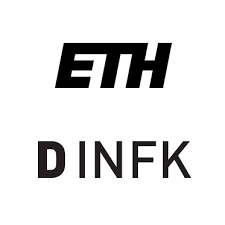
\includegraphics[width=0.2\textwidth]{eth-logo.png}\\[1cm] % Include a department/university logo - this will require the graphicx package
	 
	%----------------------------------------------------------------------------------------
	
	\vfill % Push the date up 1/4 of the remaining page
	
\end{titlepage}

\newgeometry{
 a4paper,
 footskip=.25in,
 total={170mm,257mm},
 bottom=15mm,
 left=15mm,
 top=15mm,
 }

%----------------------------------------------------------------------------------------
\section*{Disclaimer}
This summary is based strongly on the book \textit{Computer Networking - A Top-Down Approach (7th edition)} by James Kurose and Keith Ross as well as the 
lectures of \textit{Computer Networks} from the spring semester 2022. This is a personal summary and therefore I cannot guarantee completeness or correctness of the content.\\
Any constructive feedback is welcome and you can reach me under \href{mailto:jan.stauffer@inf.ethz.ch}{jan.stauffer@inf.ethz.ch}.
\newpage

\tableofcontents
\newpage

\section{Computer Networks and the Internet}
\subsection{What is the Internet}
The internet is a computer network that consists of three different things. It consists of \textbf{hosts or end systems, switches and routers, and interconnects.} End systems access the Internet through an \textbf{Internet Service Provider (ISP)}. End systems are further divisible into \textbf{clients and servers}, where clients tend to be user machines while servers are more powerful machines that provide a service.\\
To connect the end systems to the core network there has to be some kind of connection. One type of broadband residential access is \textbf{digital subscriber line (DSL)} that uses the given connection of twisted pair telephone lines. DSL consists of three different channels
\begin{itemize}
\item A high-speed downstream channel, in the 50 kHz to 1 MHz band
\item A medium-speed upstream channel, in the 4kHz to 50 kHz band
\item An ordinary two-way telephone channel, in the 0 to 4 kHz band
\end{itemize}
If the internet access is over DSL, the telephone company (telco) also acts as the ISP. Each costumer has a DSL modem that translates the digital data and translates in to high frequency tones for transmission over the telephone wires to the \textbf{central office (CO)}. In the CO, the signal of many households is received and translated back to digital format by a \textbf{digital subscriber line access multiplier (DSLAM)}.\footnote{An analog signal can take an infinite number number of values generally bound to a range while a digital signal can only take a finite number of distinct signal levels.} \\
Another way to get internet access is over cable. The \textbf{cable Internet access} makes use of the cable television company's existing cable infrastructure. There we usually have fiber cables from the CO to several neighborhood-level junctions, from which the homes are then reached via coaxial cables. This is also referred to as \textbf{hybrid fiber coax (HFC)}. The fiber connections are then terminated in the CO by a \textbf{cable modem termination system (CMTS)}  that has similar functionality to the DSLAM in DSL. One important characteristic of cable Internet access is that it is a shared broadcast medium, this means that every packet sent by the head end travels downstream on every link to every home.\\
A third and most modern way to access the internet that provides higher speeds than the former two is \textbf{fiber to the home (FTTH)}. It provides an optical fiber path from the CO directly to the home. 

\subsection{Physical Media}
Physical media are divided into two subcategories, \textbf{guided and unguided}. With guided media, the waves are guided along a solid medium, such as fiber-optic cable, a twisted-pair copper wire, or a coaxial cable. With unguided media, the waves propagate in the atmosphere and in outer space, such as in a wireless LAN or a digital satellite channel.

\subsubsection{Twisted-Pair Copper Wire}
This is the least expensive and most commonly used guided transmission medium. It consist of two insulated copper wires, each about 1 mm thick, arranged in a regular spiral pattern. The wires are twisted to reduce the electrical interference from similar pairs close by. Typically, a number of pairs is bundled together in a cable and wrapped by a protective shield. Twisted pair supports data rates from 10 Mbps to 10 Gbps and depends on the thickness of the wire and the distance of receiver and transmitter. It has emerged as the dominant solution for high-speed LAN networking.

\subsubsection{Coaxial Cable}
A coaxial cable also consists of two copper conductors that are arranged concentric rather than parallel. The cable has a copper core, then some insulating material and a braided outer conductor. The entire cable is shielded for better performance. It is quite common in cable television systems. The data rates are at tens of Mbps. Coaxial cables can be used as a guided \textbf{shared medium}, with several end systems being connected and each of them receiving what is sent by others.

\subsubsection{Fiber Optics}
An optical fiber is a thin, flexible medium that conducts pulses of lights. A single optical fiber can support data rates of up to hundreds of Gbps. They are immune to electromagnetic interference and have very low signal attenuation up to 100 kilometers and are very hard to tap. Fiber optics is prevalent in the backbone of the Internet. However, its high cost (especially of optical devices) has hindered its deployment for short-haul transport, such as LAN.

\subsubsection{Wireless}
A wireless transmitter transmits its data by emitting electromagnetic waves in many directions. One wireless sender may reach many recipients. Nearby signals that are at the same frequency interfere at a receiver. Therefore the use of the link has to be coordinated. The electromagnetic spectrum is divided into frequency bands and allocated for certain uses. Depending on the frequencies, the signals have different characteristics. Higher frequencies allow for higher data rates but are blocked by obstacles more easily. 


\subsection{The Network Core}
There are two fundamental approaches to moving data through a network of links and switches: \textbf{circuit switching} and \textbf{packet switching}.

\subsubsection{Packet Switching}
In a packet switched network, the data to be exchanged is divided into \textbf{packets}. Each packet then travels through communication links and \textbf{packet switches} which are mainly \textbf{routers} and \textbf{link-layer switches}. The packets are transmitted over each communication link at a rate equal to the full transmission rate of the link. \\
The packet switches use a \textbf{store-and-forward transmission} at the inputs of the links. This means a packet can only be forwarded if the entire packet has been received. To achieve this, there is a buffer for each incoming link where the packet can be temporarily stored. Similarly, there is a buffer at each outgoing link where packets are stored before they can be pushed onto the link. The time a packet spends in the \textbf{output buffer} is called \textbf{queueing delay}. If there are more packets to be sent than fit into the buffer, the packets are \textbf{dropped} which results in \textbf{packet loss.}\\
The packet switches somehow have to determine the outbound link on which a packet has to be forwarded. To achieve this, each end system on the internet has an address called \textbf{IP address}. The destination address is included in the packet header. Each router then has a \textbf{forwarding table} that maps each destination address to an outbound link. When a packet arrives, the router examines its destination address and puts it onto the corresponding link. The process of filling those forwarding tables are done according to special \textbf{routing protocols}.

\subsubsection{Circuit Switching}
In a circuit switched network the resources along a path are reserved. When two hosts want to communicate, the network establishes a dedicated \textbf{end-to-end connection} between the two hosts. This connection then reserves part of the links data rate it can use. Multiplexing, supporting multiple connections at a time over the same interconnect, can be achieved either by \textbf{frequency-division multiplexing (FDM)} or \textbf{time-division multiplexing (TDM)}, where either the frequency band or the time dimension is divided into frames respectively. The end systems can then send their data in the assigned frequency frame or during the assigned time slots.

\subsubsection{Circuit Switched Versus Packet Switched}
There are fundamental differences between the two approaches. Packet switched networks deliver the data by best effort without giving any guarantees, whereas circuit switched networks give guarantees. However, packet switching is seen to be more resource efficient. Circuit switched networks waste their bandwidth in \textbf{silent periods} where the end systems do not send any data. Since the resources are reserved, no other entity can make use of the available link capacity. This means if an end system wants to send data, it can only do so with its given capacity, even if there is more available when unused. Since not all users are active at the same time, a packet switched network can statistically give almost the same guarantees as circuit switched networks while accommodating more users and providing better speed. 

\subsubsection{A Network of Networks}
Each end system connects to the internet via an access ISP. But since not everyone connects to the same ISP, the different ISPs have to be interconnected as well. This can happen either directly if two ISPs \textbf{peer} or via a \textbf{provider ISP}. The ISPs form a hierarchical network of their own. Two ISPs can peer together, this means they interconnect their networks at so called \textbf{Internet Exchange Points}. Another option is to connect to a \textbf{provider}, in that case the \textbf{customer} ISP connects to the higher level provider ISP at a \textbf{point of presence}. An ISP can also \textbf{multi-home}, this means that it connects to multiple provider ISPs. This gives us a network of ISPs, where access ISPs are customers to regional ISPs, which in turn are customers to \textbf{tier-1 ISPs}. Peering connections are usually settlement free, while the customer pays the provider a fee for the data that flows over the provider ISP.

\subsection{Network Metrics}
A network connection is characterized by its \textbf{delay}, \textbf{loss rate, and throughput.}

\subsubsection{Delay}
As a packet travels through a network, it passes several routers and switches until it arrives at its destination, if at all. During this journey, the packet experiences different kinds of delay at each node along the path. The most important of these delays are \textbf{nodal processing delay, queuing delay, transmission delay, and propagation delay.} Accumulated these give the \textbf{total nodal delay.} \vspace{.3cm}\\
\noindent \textbf{Processing Delay}\\
The processing delay is the amount of time the packet switch requires to perform various computations. The most important one being the inspection of the packet's header and determining where to direct the packet. The processing delay can also include the time needed to check for bit-level errors for example.\vspace{.3cm}\\
\noindent \textbf{Transmission Delay}\\
The transmission delay is the amount of time needed to push the packet onto the link. Let $L$ be the size of the packet in bits and $R$ the transmission rate of the link in bits/sec. The transmission delay is then given by $L/R$.
\vspace{.3cm}\\
\noindent \textbf{Propagation Delay}\\
The propagation delay is the time needed by the signals to travel through the link. The signals propagate at the speed of the link. The propagation delay is given by $d/s$ where $d$ is the distance between the sending and the receiving system and $s$ is the speed of the link.
\vspace{.3cm}\\
\noindent \textbf{Queueing Delay}\\
The queueing delay is the time the packet waits to be transmitted in the output buffer. The length of the queueing delay of a specific packet will depend on the number of packets that have been received beforehand and need to be sent onto the same link. If no other packet is currently being transmitted, the queueing delay will be zero. On the other hand if traffic is heavy, the queueing delay will be long. Since the length of the queueing delay depends on the other packets in the network, it is very difficult to analyse on a per-packet basis. Therefore, in order to quantify the queueing delay statistical measures such as average, variance and probability of excess are used.\vspace{.2cm}\\
The queueing delay can be large or insignificant depending on the intensity of the traffic. Let $a$ denote the average rate at which packets arrive in packets/sec, $R$ the transmission rate of the link in bits/sec, and $L$ the size of a packet in bits. The ratio $La/R$ is called \textbf{traffic intensity}. If the traffic intensity $La/R > 1$ is greater than 1, more data arrives than can be pushed on the outward link. This means the queue is going to grow unbounded. If the traffic intensity is below 1, the queue will shrink. But since $a$ is only the average rate of packet arrival, it does not mean the queue cannot grow. In bursty traffic, the traffic intensity can be above 1 for short timeframes where the queue is going to grow and below 1 in other timeframes where the queue is going to shrink. While the traffic intensity is not a good metric for the queuing delay of a single packet but it is indicative of the average queueing delay, which grows rapidly as the traffic intensity approaches 1. \\
Because the size of the queue is not infinite, the packet switch will have to \textbf{drop} packets if the queue is already full. Those packets will be lost. This means the traffic intensity has to be below the point, where the average queueing delay is larger than our queue.
\vspace{.4cm}\\
Which kind of delay has the most impact can be different from link to link and from time to time. If we look at the end-to-end delay between two end systems that are connected via $N$ links, it is quite intuitive that we just add up all the delays at each node to get the total delay.

\subsubsection{Throughput}
End-to-End throughput is another important performance measure in computer networks. The \textbf{instantaneous throughput} at any instant of time is the rate in bits/sec, at which a host is receiving the data. The \textbf{average throughput} is the size of the data divided by the time to transmit the entire data. Some applications desire to have a low delay and an instantaneous throughput consistently above some threshold. For other applications the delay is not so important and the highest possible throughput is desirable. If no other entities are sending on the same link, the throughput is the transmission rate of the link. \\
Throughput gets interesting as soon as multiple systems and interconnects are involved. Consider two hosts connected by two links. The end-to-end throughput is the data rate of the lower link, the so called \textbf{bottleneck link}. This is generalizable, with two systems being connected by $N$ links, the end-to-end throughput is given by the lowest data rate of any of the links. The throughput is however not given by the capacities of the links alone. If a link is shared between different entities, only part of the link capacity can be used by each entity. This means a shared link could become the bottleneck link, even if it does not have the lowest transmission rate.

\subsection{End-To-End Principle}
If the network does not provide reliable transport, every application needs to engineer the reliability properties from scratch which is wasteful. But what if the network provided reliability? One issue with this is that some applications might desire a low latency connection, even if it is a bit lossy. Another problem is that the reliability of the connection depends on the the reliability of the network and the hosts as well, both of which can fail. Additionally, even if the probability of failure is low on each link, if the packet passes enough links the total chance will always be relevant, but the amount of retries can be reduced. In the end, reliability in the network...
\begin{itemize}
\item does not reduce end-host complexity
\item does increase network complexity
\item often imposes overhead for apps that don't need it
\item but can enhance performance in some cases
\end{itemize}

\subsubsection{Fate-sharing Principle}
The fate-sharing principle is an engineering design philosophy where related parts of a system are yoked together, so that they either fail together or not at all. It suggests that it is acceptable to lose the state information associated with an entity if, at the same time, the entity itself is lost.

\subsection{Network Layering}
Network protocols are organized in \textbf{layers.} This is done to provide structure, modularity and abstraction. Each protocol belongs to one of the layers. Each layer offers a service to the layer above and uses services from the layers below. This is the so-called \textbf{service model} of a layer. Layering allows for changes in the implementation of each layer without the need to change the layers above or below. The network \textbf{protocol stack} is divided into five layers, the physical, link, network, transport, and application layer.

\subsubsection{Application Layer}
The application layer is where network applications and their application-layer protocols reside. Common protocols are HTTP, SMTP, or FTP. An application-layer protocol is distributed over multiple end systems, with the application in one end system using the protocol to exchange packets of information with the application in another end system. We refer to such a packet of information at the application layer as a \textbf{message.}

\subsubsection{Transport Layer}
The transport layer transports application-layer messages between application endpoints. In the Internet there are two transport protocols, TCP and UDP. We refer to a transport-layer packet as a \textbf{segment}.

\subsubsection{Network Layer}
The network layer is responsible for moving network-layer packets known as \textbf{datagrams} from one host to another. The network layer includes the well-known IP protocol. It is responsible to determine how to deliver transport-layer packets from one system to another. It also contains numerous routing protocols.

\subsubsection{Link Layer}
The network layer routes datagrams through a series of routers between the source and destination. To move a packet from one node to another, the network layer relies on the services of the link layer. The services provided by the link layer depend on the specific link-layer protocol that is employed over the link. These protocols include Ethernet or WiFi. We refer to a link-layer packet as a \textbf{frame}.

\subsubsection{Physical Layer}
The job of the physical layer is to move individual bits of link-layer frames over a physical medium from one node to the next. The protocols are dependent on the actual transmission medium of the link.

\subsubsection{Encapsulation}
As the packet is passed up or down the protocol stack, each layer adds or removes layer specific headers. Those headers contain layer specific information that are needed to provide the service. An application-level package is encapsulated three times to get a link-layer frame, which can then be sent by the physical layer. A link-layer switch is then going to look at the metadata of the frame to determine how to process it. A network-layer router is going to unpack the datagram that is encapsulated in the frame to look at the routing information it contains. To send it onward, the router reencapsulates the datagram and passes it down to the link layer once again. At the end system, all layers of encapsulation are unpacked to recover the application-layer message.

\section{Application Layer}
Network applications are the reason the Internet exists at all. If there were no meaningful applications to implement, there would not be a need to construct an interconnected network such as the Internet.

\subsection{Principles of Network Applications}
There are two different design architectures of network applications. In a \textbf{client-server architecture}, there is an always-on host called the server, which provides a service to many other hosts, called clients. Because there is only a single instance that provides the service, this system has to be very powerful to handle the, potentially massive, amount of requests coming in. \\
The other architecture is the \textbf{peer-to-peer architecture (P2P)}. In this architecture, there is minimal or no reliance on dedicated servers. Instead the application exploits direct communication between pairs of intermittently connected hosts, called peers. The peers are not controlled by the service provider but are rather users themselves. The benefit of P2P architectures is their \textbf{self-scalability}, but it lacks in security, performance and reliability due to their highly decentralized structure.\vspace{.3cm}\\

Since applications come in all shapes and forms, they might have different requirements for the transport layer. There are different properties a transport layer protocol can provide which are desirable for certain applications. In some applications it is crucial that all the data is transmitted reliably, without loss. Those applications require \textbf{reliable data transfer.} On the other hand, \textbf{loss-tolerant applications} might not care that not the entirity of the data is transmitted reliably. The loss of data might result in a small glitch but not a crucial impairment.\\
\textbf{Bandwith-sensitive applications} require a guaranteed throughput of some specified rate. If the network cannot guarantee this throughput, the application may be unusable. \textbf{Elastic applications} can make use of as much, or as little, throughput as happens to be available. They work perfectly fine, even if the available throughput fluctuates.\\
Applications might also require certain timing guarantees to be usable. If the guarantees are not met, there is a noticable delay between action and response. A lower delay is always preferable to a higher delay, but non-real-time applications place no constraint on timing.\\
Transport protocols can also guarantee secure transport. The transport layer can encrypt all data that is transmitted by the sending process and decrypt it at the receiving process.

\subsection{Domain Name Service (DNS)}
Every end system on the network is identified by an IP address. However, those IP addresses are not very easy to remember. We humans prefer more mnemonic names since they are easier for us to remember. DNS provides quite a few services:
\begin{itemize}
\item \textbf{Host aliasing} - A host with a complicated hostname can have one or more alias names. This means a hostname is just an alias for a more complicated hostname. The original, complicated hostname is said to be the \textbf{canonical hostname}. This can also be used to reuse the machine when multiple applications are hosted on the same machine under different hostnames.
\item \textbf{Mail Server Aliasing} - For obvious reasons it is desirable to have a simple mail address. The mail server however may have a very different, more complicated canonical hostname. DNS can be invoked by a mail application to obtain the canonical hostname for a supplied alias hostname, as well as the IP address of the host.
\item \textbf{Load distribution} - DNS can also be used to perform load distribution among replicated servers, such as replicated web servers. This is done by mapping a single hostname to multiple IP addresses. Instead of a single IP, the DNS server then returns a set of addresses the client can choose from.
\end{itemize}

DNS is a distributed database that maps \textbf{hostnames} to IP addresses. A naive approach to this is to maintain a single file \textit{hosts.txt} that keeps all tuples of hostnames and matching IP addresses. This is however, not scalable. Such a file would become extremely large and would be hard to manage and keep consistent. This file would also have to be downloaded from an authoritative server, which sparks availability concerns. \vspace{.3cm}\\
To make the DNS scalable, it uses three intertwined hierarchies. It is organized hierarchical in terms of the naming structure, the management and the infrastructure. There are three different types of nameservers.\\
At the very top are the \textbf{Root DNS servers.} There are 13 root name servers managed by 12 independent organizations. The root name servers know of all TLD nameservers. To scale root servers, the operators rely on \textbf{BGP anycast}. There are currently, 1644\footnote{Valid as of 14.03.2023} instances scattered over the globe. This means that for each root server, all of its instances will announce the same prefix. Global routing will then route the traffic to the nearest instance announcing that prefix. This allows for seamless replication of resources.\\
The \textbf{Top-level domain (TLD) servers} manage their respective top-level domains such as com, org, net, edu, gov, and all the country top-level domains such as ch, uk, fr. The TLD servers provide the IP addresses for authoritative DNS servers of hostnames in their given TLD.\\
The \textbf{Authoritative DNS servers} are responsible to store the IP addresses for the hostnames they are authoritative of. Each publicly accessible domain must provide two authoritative name servers that house its DNS records. One option is to manage an own authoritative nameserver, or alternatively have these records stored in an authoritative DNS server of some service provider.\vspace{.3cm}\\
Another important type of DNS servers is the \textbf{local DNS server}. The local DNS server does not strictly belong to the hierarchy, but is still central to the DNS architecture. Each ISP, residential or institutional, has a local DNS server. When a host connects to an ISP, the ISP provides the host with the IP addresses of one or more of its local DNS servers (typically through DHCP). \\
If a host has to resolve a name, it sends a request to the local DNS server. This name server then resolves the hostname by referring to its cache or asking the root nameservers and going down the hierarchy over TLD name servers and authoritative name servers. There are two options to resolve DNS queries, \textbf{recursive and iterative.} In a recursive query, the queried server will look up the next name server in the hierarchy and query that server directly. This server then continues the lookup recursively. Once the recursive lookup has returned, the result is then forwarded to the client. In an iterative query, the name server does not continue the lookup itself, but rather returns the IP address of the next DNS server in the hierarchy for the client to continue the lookup.\vspace{.3cm}\\

A DNS server stores different types of records. The goal of the different types is to provide the different services mentioned above. A record is a four-tuple containing the fields (Name, Value, Type, TTL). The TTL is the \textbf{time to live} entry that specifies for how long a resource is valid and when it should be removed from the cache.
\begin{itemize}
\item \textbf{A records} - An A record stores a hostname in \textit{Name} and the an IP address for the hostname in \textit{Value}. This type of record therefore provides the standard hostname-toIP mapping.
\item \textbf{NS records} - A NS record stores the hostname of an authoritative DNS server that knows how to obtain the IP addresses for the hosts in the domain. This record is used to route DNS queries further along in the query chain. The \textit{Name} attribute is a domain and the \textit{Value} is the hostname of the authoritative name server. To prevent circular dependencies, since the name server of the domain might have the same domain as the hostname itself. \textbf{Glue records} have to be inserted, glue records are records of type A that provide the IP addresses of the authoritative name servers.
\item \textbf{CNAME records} - A CNAME record stores a pair of an alias hostname and a canonical hostname. The \textit{Value} attribute is the canonical hostname and the \textit{Name} attribute is the alias hostname.
\item \textbf{MX records} - The \textit{Value} is the canonical name of a mail server that has an alias hostname stored in \textit{Name}. These records are used to keep the alias names in mail addresses mnemonic.
\item \textbf{PTR records} - These so called pointer records are the opposite of a typical A record. They are used for reverse DNS lookups, where the user gives an IP address and tries to find the corresponding hostname. 
\end{itemize}
Now that we have seen what kind of records are stored in the DNS database, another question is how to insert records into the database. The first thing one hast to do is to acquire a domain at a \textbf{registrar}. The registrar is a commercial entity that verifies the uniqueness of the domain name and enters the domain name into the DNS database. For the registrar to do so, one has to supply it with the names and IP addresses of the primary and secondary authoritative DNS servers, where the A records are stored. The registrar ensures that the A and NS records of the authoritative name servers are entered into the TLD servers.\vspace{.3cm}\\

It may seem that there are a lot of messages required to resolve a domain name and this is certainly true in some cases. However, DNS lookups are not random and performance can be increased dramatically by \textbf{DNS caching.} The top 10\% of hostnames account for around 70\% of the lookups. This means that practical cache hit rates are around 75\%. DNS caching is very simple. In a query chain, when a DNS server receives a DNS reply, it can cache the mapping in its local memory. When the same request is encountered the next time, it can simply return the stored mapping. DNS servers usually discard cached information after a period of time, often set to two days.

\subsection{The Web}
The Web was created in 1990 by Tim Berners-Lee with the goal to provide distributed access to data. The World Wide Web is a distributed database of pages, linked together via the \textbf{Hypertext Transport Protocol (HTTP)}. The Web was, and still is, very successful because it enables everyone to self-publish content. Publishing on the Web is easy, independent, free, and accessible for everyone.\vspace{.3cm}\\
Every resource on the web is referred to by an \textbf{Uniform Resource Locator (URL)}, that is constructed as follows:
\begin{align*}
\text{protocol://hostname[:port]/directory\_path/resource}
\end{align*}
The protocol determines the protocol to be used to access the resource, such as HTTP(S), FTP or SMTP. The hostname addresses the destination host, which can be an IP address or a domain name. The port is optional, as it is usually derived from the protocol's standard. The directory path and resource identify the resource on the destination.

\subsubsection{Hypertext Transport Protocol (HTTP)}
HTTP is a rather simple, synchronous request-response protocol. It is layered over a bidirectional byte stream such as TCP or QUIC. HTTP is text-based and human readable. Also HTTP is stateless, it maintains no information about past client requests.\vspace{.3cm}\\
A HTTP request consists of several fields. The client specifies the request method, the URL and version as well as additional headers and a message body containing the data to be sent to the server.
\begin{figure}[H]
\centering
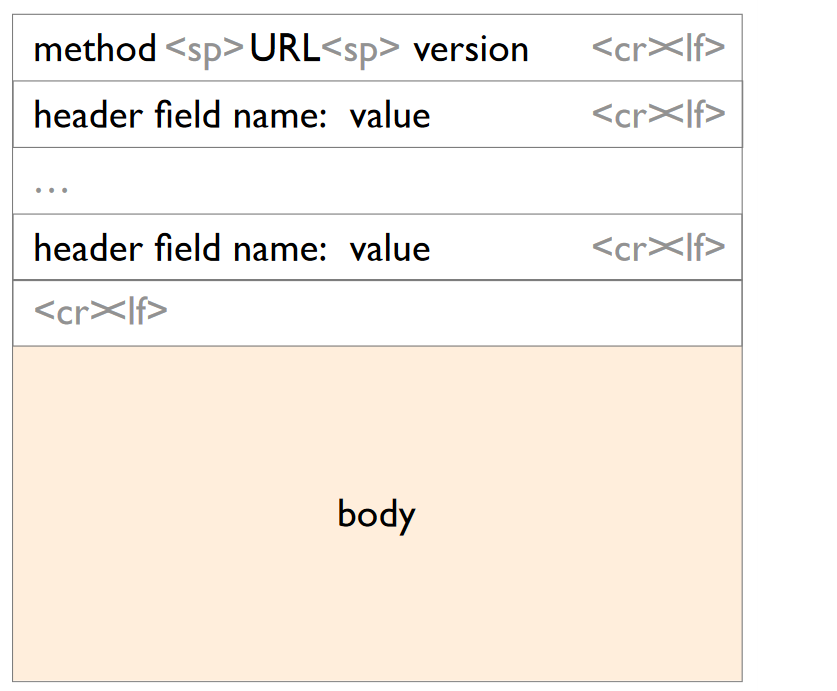
\includegraphics[width=.5\textwidth]{images/http-request.PNG}
\label{http_request}
\caption{HTTP Request Message}
\end{figure}
HTTP provides three different request methods:
\begin{itemize}
\item \textbf{GET} - returns the resource
\item \textbf{HEAD} - returns only the headers
\item \textbf{POST} - sends data to the server (forms)
\end{itemize}
The header fields are of variable lengths, but still human readable. They specify things such as
\begin{itemize}
\item Authorization Information
\item Acceptable document types/encodings
\item From (user email)
\item If-Modified-Since
\item Referrer (cause of request)
\item User Agent (client software)
\end{itemize}

The server then replies with an HTTP response. The response includes the protocol version, a \textbf{status code} and a corresponding phrase. Additionally, it returns header fields and a message body containing the requested resource. HTTP has five different types of status codes, corresponding to the state of the request.
\begin{figure}[H]
\begin{minipage}[t]{.5\textwidth}
\centering
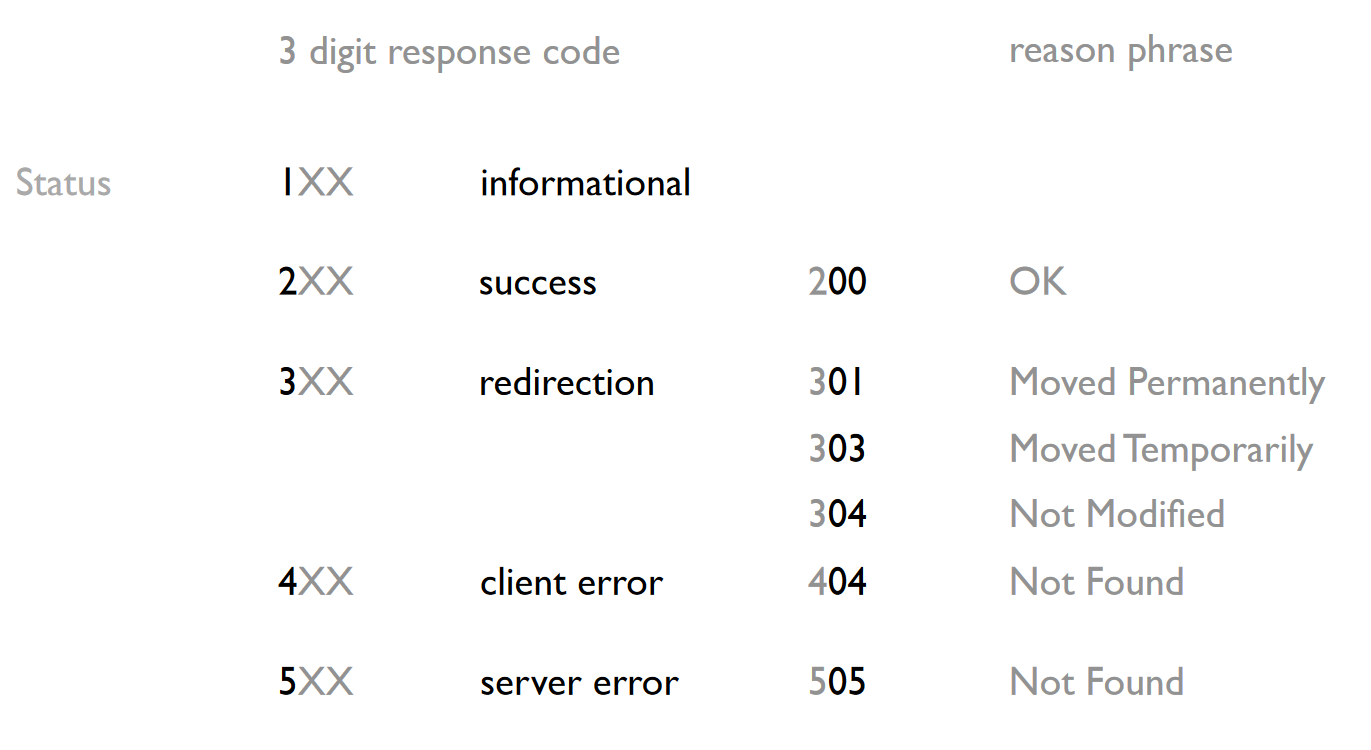
\includegraphics[width=\textwidth]{images/http-status.PNG}
\subcaption{HTTP Status Codes}
\label{http_status}
\end{minipage}
\begin{minipage}[t]{.5\textwidth}
\centering
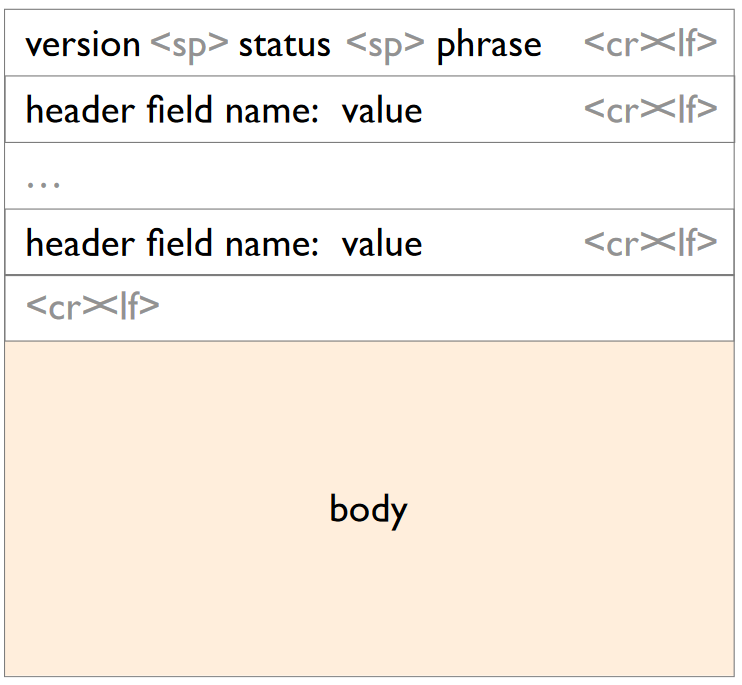
\includegraphics[width=\textwidth]{images/http-response.PNG}
\subcaption{HTTP Response Message}
\label{http_response}
\end{minipage}
\end{figure}
Like request headers, the response headers are of variable lengths and human-readable. They specify things such as
\begin{itemize}
\item Location (for redirection)
\item Allow (list of methods supported)
\item Content encoding
\item Content-Length
\item Content-Type
\item Expires (caching)
\item Last-Modified (caching)
\end{itemize}
HTTP is a stateless protocol, this makes the server-side scalable and failure handling trivial. However, some applications need state. HTTP makes the client maintain the state over so-called \textbf{cookies}. Cookies are small tokens that store state, these cookies are then sent to the server in all future requests. The server then either extracts the state from the cookie or uses the cookie to index into the state stored server-side. The server asks the client to store a cookie via the Set-Cookie header.

\subsubsection{Page Dependencies}
Web pages are far from simple and can contain many resources such as images, videos or scripts. Between these resources can be dependencies, this means that one resource can only be processed after a previous resource has finished processing. Unless it is clear that two resources are independent, the browser has to be conservative and assume dependence. \\
Those dependencies determine the load time of a page. We can model the time it takes to download and process these resources on a time-annotated dependency graph. The loading and processing of each resource represents a node in the graph. There is an edge between two nodes if there is a dependency between the two processes. For example the processing of a resource depends on the loading of that same resource. The weight of an edge is determined by the time it takes to load or process the resource it depends on. Every resource relies on at least the processing of the first resource and we introduce a FIN node that depends on every resource. This gives us a directed acyclic graph. The load time is determined by the longest path from the finish to the start. To determine the longest path we can compute a topological ordering and then determine the distances to the start node. This longest path is called the \textbf{critical path.} Speeding up any task on the critical path will either speed up the end-to-end process or reveal a different critical path.\vspace{.3cm}\\

There are many different possibilities to speed up Web browsing.
\begin{itemize}
\item Simplify, restructure, redesign Web pages\\
The resources of a page can be made faster to load by using compression and image codecs. It is also possible to inline, JavaScript and CSS, which reduces the amount of resources that have to be loaded. This obviously comes at the cost of maintainability. Another approach is to make the loading of resources independent, such that they can be loaded and processed simultaneously.
\item Use faster computing devices
\item Increase network bandwidth\\
Increasing bandwidth only gives significant returns up to a few Mbps, after the returns are diminishing.
\item Make network RTTs smaller\\
Reducing \textbf{Round Trip Times (RTT)} can be difficult in a single-path Internet, but becomes possible in a multi-path Internet.
\item Simplify network protocols
\item Caching
\end{itemize}

\subsubsection{Non-Persistent and Persistent Connections}
As we have seen, HTTP runs on TCP. Because TCP is a connection oriented protocol, it has to perform a handshake before data can be transmitted. If the connection is \textbf{non-persistent}, we have to open a new TCP connection for each resource, even if those resources reside on the same server. In a non-persistent connection, the retrieval of each element costs two RTTs, to retrieve $n$ elements, this results in $2n$ RTTs. If the host is able to open $M$ TCP connections at the same time, $2n/M$ RTTs are needed. This puts a burden on the server to handle concurrent connections and these connections create contention for bandwidth.\\
An alternative is to make the TCP connnections \textbf{persistent.} Those connections are only closed when they have been idle for some time. With persistent connections, one RTT is needed to establish the connection and for every retrieved resource another RTT is needed for the HTTP request response. The last option is to pipeline requests and replies asynchronously. If the resources are reasonably small, all requests can be sent in a single TCP segment. This only needs 2 RTTs.

\subsubsection{Web Caching}
Caching leverages the fact that highly popular content largely overlaps. This is especially useful for things that do not change very often. This saves time for the browser and decreases network and server load. Of course also a significant portion of the HTTP objects are uncachable such as dynamic data, scripts, cookies, cookies, and encrypted data or there is a motivation to not cache it for example considering advertising.\\
To limit staleness of cached objects, HTTP enables a client to validate cached objects. The server hints (like TTL) when an object expires as well as the last modification date of an object. The client can then conditionally request a resource using the if-modified-since header in the HTTP request. The server compares this against last modification time of the resource and returns either \textit{Not Modified} if the resource has not changed since or \textit{OK} along with the latest version of the resource if it has changed.\vspace{.3cm}\\
This kind of caching is performed at three different locations. The first location is the clients browser, which contains a \textbf{browser cache.} The second location is close to the client, either in a so-called \textbf{forward proxy} or a \textbf{Content Distribution Network}. A forward proxy is usually maintained by the ISP, somewhere close to the users. This reduces response time and load on the network, which directly relates to less cost for the ISP. Content distribution networks are distributed networks of servers that try to localize traffic. There is a root server and a replica server, if a request goes to the CDN, the request-routing system chooses a suitable replica server and redirects the request. There are shared CDNs as well as dedicated CDNs.\\
The third location is close to the server in so-called \textbf{reverse proxies}. A reverse proxy is installed by the content provider and is in front of the server cluster. Reverse proxies help reducing the load on the actual servers by cacheing their content. A request first reaches the reverse proxy, if the content is not cached, the reverse proxy sends a request to one of the servers and retrieves the content. I assume this is also helpful to loadbalance the servers, since the proxy can choose which server to query.



\section{Transport Layer}
The transport layer sits between the application layer and the network layer. Its task is to provide an interface for (reliable) transport over a potentially unreliable medium. It tries to convert the host-to-host delivery of the network layer into a process-to-process delivery, by multiplexing and demultiplexing data. To the application layer it provides the abstraction to send files or byte-streams from application to application, by translating between packets and those forms of data. The transport layer also implements reliable transfer, flow control and congestion control.

\subsection{Reliable Transport}
The transport layer tries to provide reliable transport over a potentially unreliable connection. During transit and processing of the packets, several things can happen. Data packets can get \textbf{lost, corrupted, reordered, or duplicated}. The transport layer tries to ensure \textbf{correctness, timeliness,  efficiency, and fairness.} \vspace{.3cm}\\
A first attempt at implementing such a protocol includes a checksum to deal with corruption and each packet is acknowledged. Because such an acknowledgement could get lost too, we set a timer for each sent packet. If the timer runs out without an acknowledgement being received, the packet is resent. This protocol has a lot of practical issues. For example, how does the protocol know, which packet has been acknowledged. \vspace{.3cm}\\
We also want a formal definition of correctness, which is not trivial. \textit{A reliable transport design is correct if and only if a packet is always resent if the previous packet was lost or corrupted.} Now that we have this definition, we need to design a correct, timely, efficient and fair transport mechanism. If we focus on the aforementioned approach, we can clearly see a tradeoff between timeliness and efficiency when choosing the timeout value. Timeliness argues for small timers, since we want to retransmit lost packets as fast as possible. However, with short timers we risk unnecessary retransmissions if the timer runs out before the response arrives. Efficiency argues for slow timers, since we only want to retransmit if we really lost the packet. This comes at the cost of very slow retransmissions in case of packet loss. \vspace{.3cm}\\
This approach is a so-called \textbf{stop-and-wait}, after the protocol has sent a package, it stops and waits for the acknowledgement. Even with short timers the protocol is extremely slow and wasteful because it can only send one packet per Round-Trip Time. An obvious solution to improve timeliness is to send multiple packets at the same time. To keep order, we add a sequence number inside each packet and keep buffers at the sender and receiver. The sender stores packet that have been sent but not yet acknowledged. The receiver stores packet that have arrived out-of-sequence as well as those that have not been passed to the application yet.\\
Sending multiple packets at the same time improves timeliness but it can also overwhelm the receiver and destroy efficiency. If the sender sends more packets than the receiver can handle, those packets are dropped at the receiver, causing retransmissions that would not have been necessary if the sender sent at a slower rate.

\subsubsection{Flow Control}
To keep the sender from overwhelming the receiver, we need a mechanism called 
\textbf{flow control}. One way to do this is using \textbf{sliding windows}. The sender keeps a \textbf{sending windows} with a list of the sequence numbers it can send. The receiver keeps a \textbf{receiving window} with a list of acceptable sequence numbers. The sender and receiver negotiate the size of the windows. The sending window starts from the oldest packet that has been sent but not acknowledged. The sender may send all other packets in the window but not beyond it. When an acknowledgement for the oldest packet is received, the window slides forward. The window therefore limits the number of packets that can be in flight simultaneously. \\
The timeliness of the sliding window protocol depends on the size of the window. To maximize timeliness, the size of the window should be equal to the \textbf{bandwidth-delay product (BDP)}. The efficiency depends on the receiver feedback and how the sender uses it. There can be no feedback, in which case the protocol relies entirely on timers or the acknowledgement can be taken as feedback. There are three different ways to encode feedback into acknowledgements:
\begin{itemize}
\item \textbf{Individual ACKds} - The acknowledgement includes the number of the packet received. The lost packets with individual ACKs are implicit. The sender can infer that a packet is missing after receiving $k$ subsequent ACKs or after the timer runs out. They provide detailed feedback but can trigger unnecessary retransmissions if ACKs are lost.
\item \textbf{Cumulative ACKs} - The acknowledgement means that all packets have been received up to the given number. Cumulative ACKs are more robust to ACK loss, but it is harder to find which packets are missing. If the sender receives duplicate ACKs for a number, it can infer that the packet after is missing and send it when the timer runs out or after $k$ duplicate ACKs. The question is what to resend, only the subsequent packet or all of them. 
\item \textbf{Full information ACKs} - Combination of individual and cumulative. Full information ACKs make the missing packets explicit. The sender learns which packets are missing and can retransmit after $k$ ACKs or when the timer runs out. Full information ACKs prevent unnecessary retransmissions but incur a sizeable overhead.
\end{itemize}
Now we have seen ways to make a transport mechanism correct, timely and efficient, but what about fairness. When $n$ entities are using the transport mechanism, we want a fair allocation of the available bandwidth. Defining fairness is not trivial, usually we go with \textbf{equal-per-flow} bandwidth distribution. One might argue about the fairness of this notion, since a flow that spans more interconnects also uses more of the networks resources. However in practice, a universally agreed upon minimal goal is to avoid starvation for which equal-per-flow is good enough. To achieve this, simply dividing the available bandwidth doesn't work in practice, since different flows can see different bottlenecks. Intuitively, we want to give the users with low demands what they want and evenly distribute the rest. This \textbf{max-min fair allocation} is such that the lowest demand is maximized, after that the second lowest and so on. This allocation can be approximated by slowly increasing the window size until a loss is detected, because loss is a signal of congestion.\vspace{.3cm}\\

A simple sliding window protocol using cumulative ACKs is called \textbf{Go-Back-N}. Its goal is to make the receiver as simple as possible. The receiver delivers the packets in-order to the upper layer and for each received segment, it ACKs the last in-order packet it has received cumulatively. The sender uses a single timer to detect loss and resets the timer at each ACK. Upon timeout, it resends all packets in the window starting with the lost one. In this protocol, a lot of unnecessary retransmission occur if a single packet is lost because all subsequent packets are also resent.\vspace{.3cm}\\

Another approach that avoids unnecessary retransmissions is called \textbf{Selective Repead (SR)}. It avoids unnecessary retransmissions by using per-packet ACKs. The sender uses timers to detect packet loss and resends only the lost packets. 

\subsection{User Datagram Protocol (UDP)}
UDP is a simple extension of IP. It only provides process-to-process data delivery and optional checksums. It delivers the data to the correct application by demultiplexing using application identifiers called ports. It doesn't provide reliable transport, nor flow control, nor congestion control. The UDP header consists of four fields, a \textbf{source port, destination port, checksum and length field}. It avoids overhead and delays of ordered, reliable delivery. It has no delay for connection establishment and offers a finer control over what data is sent and when. It has no connection state, buffers, or timers leading to greater scalability and the per-packet overhead is minimal. It is used in applications such as DNS, gaming or VoIP.\\
UDP demultiplexes between sockets, which are the interface between the transport and the application layer. A UDP socket is uniquely identified by its destination address and destination port. Every packet that gets delivered to a host (which has an IP address) and has the same destination port, get delivered to the same socket by UDP. It does not distinguish where the packet comes from.

\subsection{Transmission Control Protocol}
TCP in contrast to UDP, provides all the aforementioned properties of reliable transport. It delivers data to the correct application using demultiplexing and provides file or byte-stream abstractions to the application layers, which it segments or reassembles accordingly. It implements acknowledgement and checksums as well as flow and congestion control. To ensure reliability, both sender and receiver are required to keep state in so-called \textbf{connections or sessions.} \\
The transport layer protocols cannot guarantee delay or bandwidth guarantees since those would require support at the network layer. However, some things it can guarantee without support from the network layer such as confidentiality.

\subsubsection{TCP Header}
The TCP header is a lot more complex than the UDP header. Similar to UDP it includes fields for source and destination port as well as a checksum. Apart from that it has fields for the sequence and acknowledgement numbers, length of the header, flags, advertised window size, an urgent pointer and a variable length options field.
\begin{figure}[H]
\centering
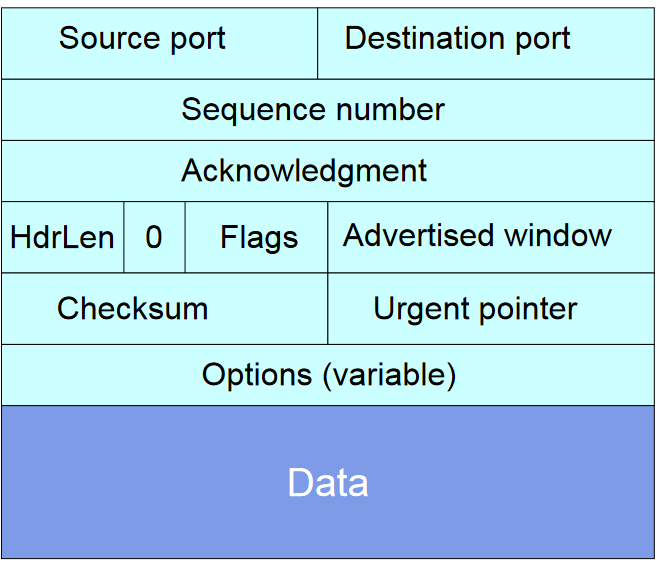
\includegraphics[width=.5\textwidth]{images/tcp_header.PNG}
\caption{TCP Header}
\label{tcp_header}
\end{figure}
TCP splits the application data into segments, a segment is transmitted when it is full or a timer runs out. The size constraints of a TCP segment come from size constraints of an IP packet, which can be no bigger than the \textbf{maximum transmission unit}. The size of the TCP segment with the IP header must be smaller than the MTU. This, along with the TCP header size gives a constraint called the \textbf{maximum segment size (MSS)}.\vspace{.3cm}\\

Ordering and acknowledgement in TCP is done with \textbf{sequence numbers} that are transmitted in the sequence number header field. During the handshake, \textbf{initial sequence numbers (ISN)} are exchanged between both participants. When sending data, the sender includes the sequence number of the first byte in the header. The sequence number of byte $n$ in the stream is $ISN + n$. Upon reception, the receiver acknowledges by setting the ACK flag and setting the acknowledgement number header field to the sequence number of the byte it expects to receive next. Intuitively, (if everything arrives in order) the sequence number of the next segment is the same as the acknowledgement number of the last segment.\vspace{.3cm}\\

\subsubsection{Connection Establishment \& Teardown}
One thing among others that happens during the connection establishment is the exchange of the initial sequence numbers. One might ask the question on why not to take zero everytime. TCP connections are identified by the IP addresses and ports of the end systems. Eventually however, these port numbers have to be reused and it is technically possible that there is an old packet still in flight. TCP therefore requires changing ISN, which are drawn from a pseudo random number generator. The connection establishment happens via a 3-way handshake. First the client sends a SYN segment (with the SYN flag set) including its ISN, the server responds with a SYN-ACK segment including its own ISN. The client acknowledges this with an ACK segment. In case the SYN segment gets lost or discarded, no SYN-ACK segment is going to arrive and the client will eventually retransmit the SYN segment. Since the client has no idea about the RTT to the server, it has to wait for a reasonable amount of time before resending they SYN. According to the standards, a default of 3 seconds should be used.
\begin{figure}[H]
\centering
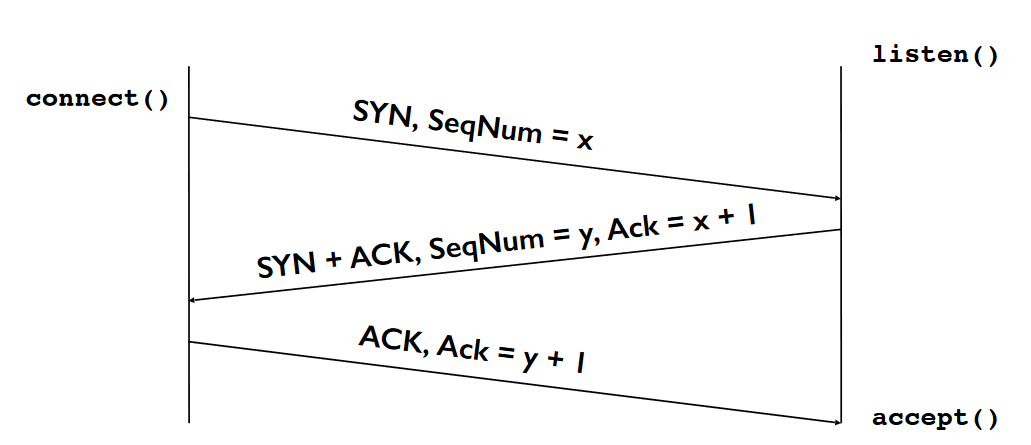
\includegraphics[width=.6\textwidth]{images/tcp_handshake.PNG}
\caption{TCP Handshake}
\label{tcp_handshake}
\end{figure}
Because the serve needs to keep a mapping of each client connection to an ISN, it opens a simple attacking strategy called \textbf{SYN flooding} where the server is flooded by SYN packets without the client ever completing the handshake. This depletes the server of its resources because it has to maintain state. A defence mechanism against this are called \textbf{SYN cookies}, which allows the server to complete the handshake without maintaining state after the first SYN segment. To do this, the server computes its ISN $y$ using a secret hashing mechanism (secrecy comes from including a secret number in the hash) using the clients identifiers. Because the client is going to acknowledge $y + 1$ the server can verify if a SYN was sent before without building state. \vspace{.3cm}\\

If one side wants to terminate the connection it sends a FIN segment and waits to receive any remaining data the other side has to send. The other side sends an ACK and transports its remaining data. If the second side is ready to terminate the connection too, it sends a FIN segment of its own which is then ACKed by the other side. After this, the connection is closed both ways. If an ACK is lost, the FIN will be retransmitted.\\
If the connection has to be terminated abruptly (e.g. because an application process crashed) the terminating side sends a RESET (RST) segment. This RST is not acknowledged and thus not delivered reliably. Any data in flight is lost and if data is received still, the RST is resent.

\subsubsection{RTT estimation}
We have seen that choosing the correct length for timeouts is crucial to timeliness and efficiency. If the timeout value is chosen too long the connection is inefficient, if it is chosen too short unnecessary retransmits occur. Hence it is important to estimate the RTT. There are several ways to do such an estimation.
\begin{itemize}
\item \textbf{Exponential Averaging} 
\begin{align*}
SampleRTT = AckRcvdTime - SendPacketTime \\
EstimatedRTT = \alpha \times EstimatedRTT + (1-\alpha) \times SampleRTT
\end{align*}
Assuming the RTT is constant, this method will correctly approach the RTT. Depending on the value of $\alpha$ this approximation happens with different speeds (lower $\alpha$ faster approximation), but it comes at the cost of higher sensitivity to fluctuation. One problem of this approach is that timings from retransmitted packages highly skew the estimation.
\item \textbf{Karn/Partridge Algorithm} - This algorithm addresses the issue of retransmitted packages and simply ignores them. It only measures $SampleRTT$ for original transmissions. Other than that it computes the estimated RTT using exponential averaging with $\alpha = 0.875$. It sets the timeout value $RTO = 2 \times EstimatedRTT$. For repeated transmissions it uses exponential backoff. Every time the RTO timer expires it doubles the RTO up to a maximum of 60 seconds. Every time a new measurement comes in, it collapses the RTO back to $2 \times EstimatedRTT$.
\item \textbf{Jacobsen/Karels improvement} - This variation also accounts for the estimated deviation (Deviation = | SampleRTT - EstimatedRTT|), where it estimates the deviation by exponential average over the deviation. It then sets the $RTO = EstimatedRTT + 4 \times EstimatedDeviation$.
\end{itemize}

\subsection{Congestion Control}
\begin{wrapfigure}{r}{.4\textwidth}
\centering
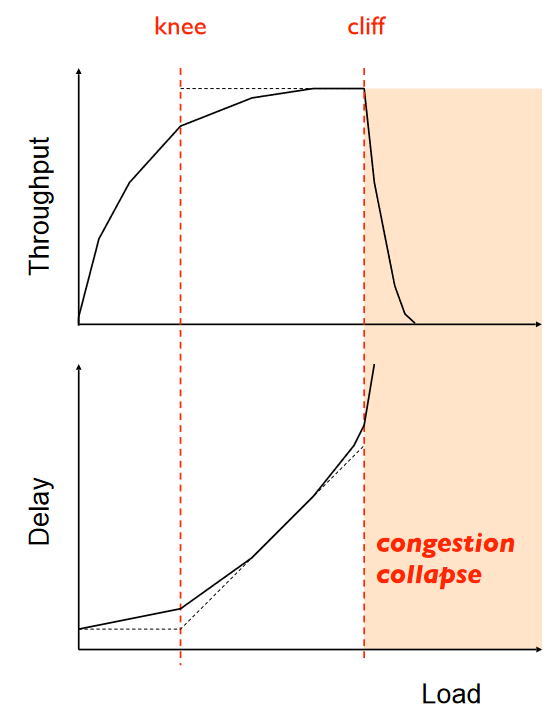
\includegraphics[width=.4\textwidth]{images/congestion_collapse.PNG}
\caption{Congestion Collapse}
\label{congestion_collapse}
\end{wrapfigure}
Because of traffic burstiness and lack of bandwidth reservation, congestion is inevitable. If many packets arrive within a short period of time, the node cannot keep up anymore. Congestion is also not a new problem, the Internet almost died of congestion in 1986. Originally, sending rate was only limited by flow control and nodes would send full windows of packets. Upon timer expiration, they would retransmit the packet immediately. This behaviour would result in window-sized bursts of packets. This sudden load would increase the RTT and as that exceeds the maximum retransmission interval, the hosts would begin to retransmit packets. Like this, hosts are sending each packet multiple times. This phenomenon is known as a \textbf{congestion collapse}. \vspace{.3cm}\\
Congestion control aims at solving three problems.
\begin{itemize}
\item \textbf{Bandwidth estimation} - How to adjust the bandwidth of a single flow to the bottleneck bandwidth?
\item \textbf{Bandwidth adaptation} - How to adjust the bandwidth of a single flow to variation of the bottleneck bandwidth?
\item \textbf{Fairness} - How to share bandwidth fairly among flows, without overloading the network.
\end{itemize}
Congestion control differs from flow control. Flow control prevents one fast sender from overloading a slow receiver. Congestion control prevents a set of senders from overloading the network. TCP solves both using two distinct windows. Flow control is solved using a receiving window, while congestion control is solved using a \textit{congestion} window. The sender then uses the smaller one of both windows as its sending window.

\subsubsection{Congestion Detection}
The first step to congestion control is the detection of congestion. There are essentially three ways to detect congestion
\begin{itemize}
\item Network could tell the source it is congested, but that signal could be lost
\item Measure the packet delay, but that signal is noisy and the delay often varies considerably
\item Measure packet loss, this is a fail-safe signal of congestion that TCP has to detect anyway
\end{itemize}
Packet dropping is the easiest solution, it is not perfect but delay- and signalling-based methods are hard and risky. As seen before, detecting losses can be done using ACKs or timeouts, the two signals differ in their degree of severity. Duplicated ACKs are a mild congestion signal, since packets are still making it. A timeout is a severe congestion signal and signifies multiple consequent losses. \vspace{.3cm}\\

TCP's approach is to gently increase when not congested and to rapidly decrease when congested. The question is, what kind of increase/decrease functions should be used? That depends on the problem we are trying to solve.

\subsubsection{Slow Start}
This method tries to solve the first problem, to quickly get a first-order estimate of the available bandwidth. Intuitively, the sender starts slow but rapidly increases until a packet drop occurs. Initially, the congestion windows starts at one. Upon reception of an ACK segment, the congestion window size is increased by one. This leads to an exponential increase of the congestion window size. The problem with slow start is that it can result in a full window of packet losses. Therefore, we need a more gentle adjustment algorithm once we have a rough estimate of the bandwidth.

\subsubsection{Congestion Avoidance \& Fairness}
After we have determined a rough estimate of the bandwidth with slow start we switch to more gentle adjustments. Essentially, there are two different variations to adjust the congestion window size. 
\begin{align*}
cwnd &= a \times cwnd \quad & \text{Multiplicative Increase or Decrease} \\
cwnd &= b + cwnd \quad & \text{Additive Increase or Decrease} 
\end{align*}
Which leaves us with four different methods to adjust the window size. Additive Increase and Additive Decrease (AIAD). Additive Increase and Multiplicative Decrease (AIMD). Multiplicative Increase and Additive Decrease (MIAD). Multiplicative Increase and Multiplicative Decrease (MIMD).
\begin{table}[]
\centering
\begin{tabular}{lll}
& {\color{gray} increase behavior} & {\color{gray} decrease behavior} \\
{\color{gray} AIAD} & gentle & gentle \\
{\color{gray} AIMD} & gentle & aggressive \\
{\color{gray} MIAD} & aggressive & gentle \\
{\color{gray} MIMD} & aggressive aggressive
\end{tabular}
\end{table}
To decide between these four options, we consider the last factor, which is fairness. It turns out that AIMD is the only method to converge to a fair and efficient allocation of the bandwidth. It then fluctuates around the optimum in a stable way. \vspace{.3cm}\\

This is why TCP implements AIMD in practice. But instead of increasing the window size by one on each received ACK, it increments the congestion window by at most one ever RTT. (cwnd = cwnd + 1/cwnd). 
Another question is, when to leave slow start and continue with AIMD. We introduce a slow start threshold $ssthresh$ and adapt it as a function of congestion. On a timeout, we set $ssthresh = cwnd/2$. Initially we set $ssthresh$ to infinity and slow start until a timeout occurs, and adjust the threshold accordingly. After this, we slow start until timeout or we reach $ssthresh$, in which case we switch to AIMD. With this strategy we would keep increasing the congestion window until a timeout, even if mild congestion signals were received. However, going back to 0 every time we receive a timeout is expensive, we might want to consider the mild congestion signals as well. TCP automatically resends a segment after receiving three duplicated ACKs for it, this is known as \textbf{fast retransmit}. After a fast retransmit, TCP switches back to AMID, without going all the way back to 0, this is known as \textbf{fast recovery}. It sets $ssthres = cwnd/2$ and starts with AIMD at $cwnd = ssthresh$.

\subsubsection{Congestion Control Algorithms}
A \textbf{congestion control algorithm (CCA)} specifies the adaptation of the sending rate in response to measured network metrics and is embedded in a transport layer protocol.
\begin{itemize}
\item \textbf{TCP Reno} - This is the classic TCP CCA as we have seen so far. It increases the congestion window by $1/RTT$ in absence of loss and cuts the congestion window in half in presence of packet loss. Since the $cwnd$ is increased based on the RTT, TCP Reno experiences something called \textbf{RTT unfairness}, where senders with long RTTs will increase their sending rate more slowly and thus obtain less bandwidth.
\item \textbf{TCP Cubic} - This is a well-established TCP CCA and is default in the Linux kernel. It is a loss-based CCA as well. It keeps a state variable $s$ to save the time since the last loss and $w_{max}$ to save the $cwnd$ at the time of the last loss. It sets $cwnd = w_{max} + 0.4(s - (0.75 w_{max})^{1/3})^3$. TCP Cubic does not experience RTT unfairness, since the growth rate is independent of the RTT. However, it experiences something called \textbf{bufferbloat}. Since the sending rate is only decreased in case of loss, the link buffers will be mostly filled independent of their size, keeping latency high.
\end{itemize}
Loss-based CCAs are inherently suboptimal since they only decrease the sending rate on loss. There is a point called the \textbf{Kleinrock optimal} operating point, where the links are filled yet the buffers kept empty. Like this, each packet arrives at an empty buffer, suffering little to no queueing delay.
\begin{figure}[H]
\centering
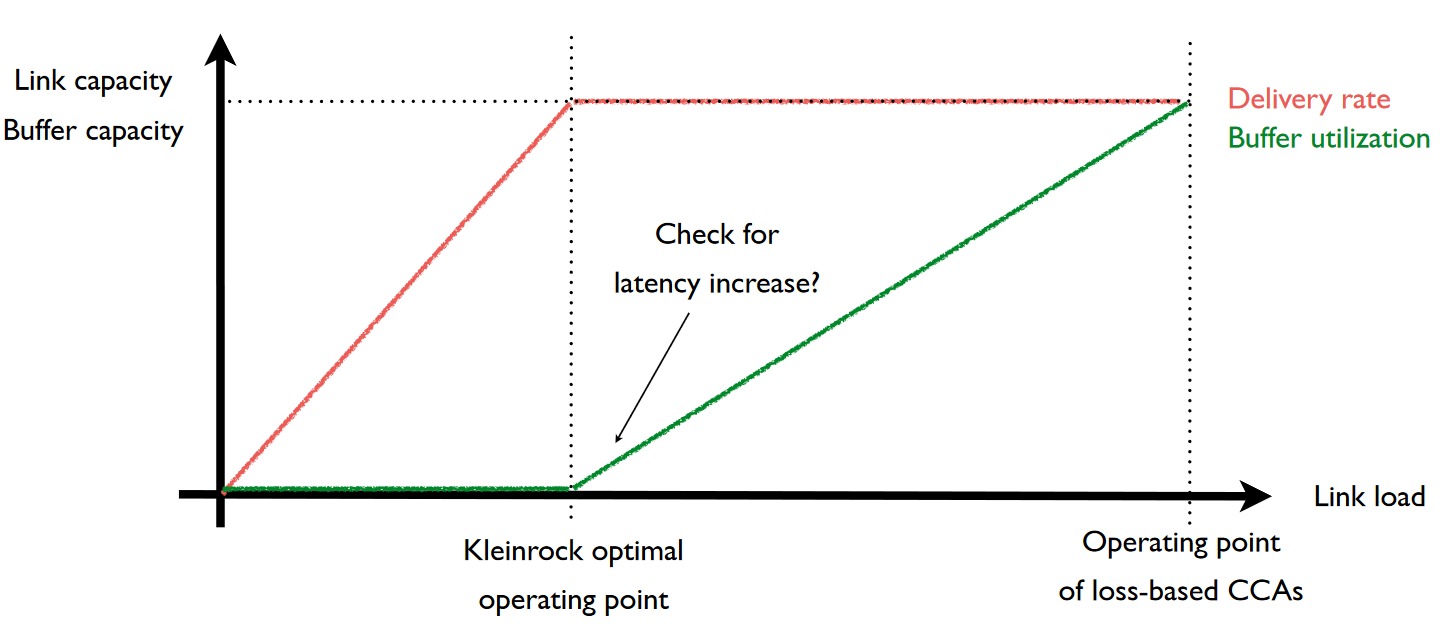
\includegraphics[width=.8\textwidth]{images/kleinrock.PNG}
\caption{Kleinrock Optimal}
\label{kleinrock}
\end{figure}
\begin{itemize}
\item \textbf{TCP Vegas} - This is a CCA designed in the 90s but it was never widely used. It implements congestion avoidance by estimating the propagation delay $T$ (min. RTT measurement) and once per RTT it measures the current RTT $T_{cur}$. It then picks $\alpha < \beta$ and adjusts the congestion window as follows:
\begin{itemize}
\item If $cwnd/T_{cur} < cwnd/(T - \beta)$, linearly decrease $cwnd$
\item If $cwnd/T_{cur} > cwnd/(T - \alpha)$, linearly increase $cwnd$
\end{itemize}
This is a latency-based CCA. Uncovering the propagation delay is difficult. The main problem with this approach however is, that this algorithm is \textbf{uncompetitive against loss-based CCAs}. The sender using TCP Vegas will reduce their sending rate as soon as they detect a latency increase, while loss-based CCA will build up their queue until they experience loss, leading to unfairness.
\item \textbf{TCP BBR} - BBR is a CCA published by Google in 2016. To avoid congestion it keeps two stae variables $BtlBw$ and $MinRTT$. It cycles through periods of eight phases. Each phase has duration $MinRTT$. In general, the sender sends at rate $BtlBw$ in each phase. In one random phase the sending rate is increased to $1.25 \times BtlBw$ and in the following phase reduced to $0.75 \times BtlBw$. At the end of the period, it updates the $BtlBw$ to the maximum observed delivery rate. This is a so-called model-based CCA. This CCA is \textbf{unfair against loss-based CCAs}. The loss-insensitive BBR probing leads to recurring loss, which makes loss-based CCAs refrain.
\end{itemize}
\begin{table}[H]
\centering
\begin{tabular}{p{2cm}p{8cm}}
\rule{0pt}{4ex} Reno & RTT unfairness \\
\rule{0pt}{4ex}  CUBIC & RTT fairness \newline not Kleinrock-optimal  \\
\rule{0pt}{4ex}  Vegas & Kleinrock-optimal \newline uncompetitive agains loss-based CCAs \\
\rule{0pt}{4ex}  BBR & Kleinrock-optimal \newline unfair against loss-based CCAs
\end{tabular}
\end{table}

\subsection{QUIC}
QUIC used to stand for Quick UDP Internet Connections. Nowadays, it is seen as the name of a new Internet protocol. TCP and UDP have been the most widely used transport layer protocols to date. QUIC tries to redefine TCP, a new way to implement reliable transport. TCP is used in billions of devices and if TCP wasn't fit for general use, we would have gone with another protocol. TCP is useful in a wide variety of cases and in many of them, it is incredibly good at its job. Part of the reason for TCP's longevity and broad adoption is TCP's flexibility, it supports a diverse variety of uses and works well in all kinds of different scenarios. But despite this considerable flexibility, TCP has its problems, especially with web-based services. Web pages are not simple monolithic objects, they typically contain many separate components. If the browser is equipped with the original implementation of HTTP, each object will be loaded in a new TCP session. The overheads of setting up both a brand new TCP session and a new \textbf{Transport Layer Security (TLS)} session for each distinct resource can become quite significant. Seeing this, it becomes reasonable to reuse an already established TLS session for multiple fetches from the same server. However, this approach of multiplexing a number of data streams within a single TCP session also has its issues. Multiplexing multiple logical data flows across a single session can generate unwanted dependencies and can lead to \textbf{head-of-line blocking}. This appears when a single logical data stream has issues, which leads to blocking of the other logical streams due to stalling of the connection. \vspace{.3cm}\\

One might think that we could simply start anew and design a new transport protocol that addresses these shortcomings. However, this is not so easy because of NATs and middleboxes. While IP allows a broad selection of different protocols, TCP and UDP (and ICMP to some degree) are the only widely accepted protocols. This means that \textbf{Network Address Translations (NAT)} are simply blocking packets that are neither UDP nor TCP. This leaves us with only two choices to implement a new transport-layer protocol, TCP and UDP.\vspace{.3cm}\\

QUIC chose the UDP based approach. Also QUIC is strictly speaking a datagram transport application. QUIC also moves the implementation of the transport protocol out of the kernel space (the OS) and into the user space (the application). With UDP there are no distinct connection establishment and termination segments for NATs to go off, which means they have to make assumptions. This means it is possible that the NAT deletes and recreates a translation table entry for the same connection with potentially different port numbers and source addresses. How can the QUIC server recognize that this next received packet, with new source address and source port number, is actually part of an existing session? QUIC uses the concept of connection identifiers, which allow the QUIC server to route the packets to the correct process. These connection IDs are generated by the endpoints and exchanged during QUIC version negotiation. These connection identifiers also allow to retain connections on IP address changes, e.g. when a mobile device changes to a different tower.\vspace{.3cm}\\

One QUIC connection can also support a number of streams with different profiles (unidirectional, bidirectional). In TCP, each stream has to be transported over a separate TCP/TLS session or over one session where head-of-line blocking can occur. In QUIC the stalling of one stream does not imply that any other simultaneous stream is affected.\\
Furthermore, QUIC encrypts a lot more of its data. While in a TCP/TLS session, only the actual payload is encrypted, QUIC encrypts everything except for a few public headers such as port numbers, flags and connection identifiers.\vspace{.3cm}\\

QUIC also has its downsides. For example, QUIC packets are fixed size. This means that the packets can not be fragmented. The QUIC HELLO packet is padded out to the maximal packet size, if this HELLO exchange fails if the packet has to fragmented. In this case application falls back to a simultaneously established TCP session.

\section{Network Layer - Data Plane}
The transport layer provided process-to-process communication relying on the network layer without knowing anything about the network. The network layer provides the host-to-host transport the transport layer builds on. The protocols of the network layer are implemented in every single router in the network. The network layer implements routing protocols, that determine, how to route a packet through the network from its source to its destination. The functionality of the network layer can be divided into a \textbf{data plane} and a \textbf{control plane}. The role of the data plane is the implementation of \textbf{forwarding} on a per-router basis. Forwarding is the process of sending a packet from an incoming link to the next router in the path over an outgoing link. The role of the data plane is the \textbf{routing}, the coordination of these local, per-router forwarding actions to achieve end-to-end transfer along paths of routers. Forwarding and routing are often used interchangeably. However in this course, forwarding refers to the router-local action of transferring a packet from an input link interface to the appropriate output link interface. Routing refers to the network-wide process that determines the end-to-end paths. A key element in every network router is its \textbf{forwarding table.} A router forwards a packet by examining the value of one or more fields in the arriving packet's header, and then using these header values to index into its forwarding table.

\subsection{IPv4 Datagram Format}
A packet on the Internet's network-layer is referred to as a \textbf{datagram.} They key fields in the IPv4 datagram are the following:
\begin{itemize}
\item \textbf{Version Number} - These four bits specify the IP protocol version of the datagram. The two widely used IP versions are IPv6 and IPv6.
\item \textbf{Header Length} - Because an IPv4 datagram can contain a variable number of options, these 4 bits are needed to determine where in the IP datagram the payload actually begins. Most IP datagrams do not contain options, so the typical IP datagram header is 20 bytes long.
\item \textbf{Type of Service} - The type of service (TOS) bits were included in the header to allow different types of IP datagrams to be distinguished from each other. For example to distinguish real-time datagrams from non-real-time traffic. 
\item \textbf{Datagram Length} - This is the total length of the IP datagram (header plus data) measured in bytes. Since this field is 16 bits long, theoretical maximum size of the IP datagram is 65'535 bytes. However, datagrams are rarely larger than 1'500 bytes, which allows an IP datagram to fit in the payload field of a maximally sized Ethernet frame.
\item \textbf{Identifier, flags, fragmentation offset} - These three fields have to do with so-called IP \textbf{fragmentation}. IPv6 does not allow for fragmentation.
\item \textbf{Time-to-Live} - The time-to-live (TTL) field is included to ensure that datagrams do not circulate forever. This field is decremented by one each time the datagram is processed by a router. If the TTL field reaches 0, a router must drop that datagram.
\item \textbf{Protocol} - This field is typically used only when an IP datagram reaches its final destination. The value of this field indicates the specific transport-layer protocol to which the data portion of this IP datagram should be passed. For example, a value of 6 indicates TCP, while a value of 17 indicates UDP. 
\item \textbf{Header Checksum} - The header checksum aids a router in detecting bit errors in a received IP datagram. The checksum is calculating by treating each two bytes as an integer and summing them using 1's complement arithmetic. This checksum is typically recomputed at every step since fields like the TTL or others change.
\item \textbf{Source and Destination IP Addresses} - When a source creates a datagram, it inserts its IP address into the source IP address field and inserts the address of the ultimate destination into the destination IP address field. Often the source host determines the destination address via a DNS lookup.
\item \textbf{Options} -  The options fields allow an IP header to be extended. Header options were meant to be used rarely - hence the decision to not include the information in option fields in every datagram header. However, the mere existence of options does complicate matters, especially for high-performance routers and hosts. For these reasons and others, IP options were not included in the IPv6 header.
\item \textbf{Data} - In most circumstances, the data field of the IP datagram contains the transport-layer segment (TCP or UDP) to be delivered to the destination. However, the data field can carry other types of data, such as ICMP messages.
\end{itemize}
\begin{figure}[H]
\centering
\includegraphics[width=.5\textwidth]{images/IPv4_header.PNG}
\caption{IPv4 Datagram Header}
\label{ipv4_header}
\end{figure}

\subsection{IPv4 Datagram Fragmentation}
Not all link-layer protocols can carry network-layer packets of the same size. For example, Ethernet frames can carry up to 1'500 bytes of data, whereas frames for some wide-are links can carry no more than 576 bytes. The maximum amount of data that a link-layer frame can carry is called \textbf{maximum transmission unit (MTU)}. IP datagrams are encapsulated within link-layer frames, hence the MTU of the link-layer protocol places a hard bound on the length of an IP datagram. This is not much of a problem,  what is a problem is that some links along the network path can have different MTUs. If the outgoing link-layer protocol has a smaller MTU than the current IP datagram, the datagram has to be split up into smaller IP datagrams. These smaller datagrams are referred to as \textbf{fragments.} These fragments need to be reassembled before they are passed to the transport-layer protocol. The reassembly happens in the end systems rather than the network itself. When a host receives IP datagrams it has to determines if any of them belong to a bigger original datagram. To allow the destination host to perform these reassembly tasks, the IP datagram header includes the identification flag and a fragmentation offset. Each datagram gets a identification number upon creation, when a router needs to fragment a datagram, each resulting datagram receives the same identification number. Because the network can lose fragments, the last fragment has a flag bit set to 0 while all other fragments have it set to 1. The receiving host determines whether a fragment is missing by looking at the fragmentation offset.

\subsection{IPv4 Addressing}
A host typically has only a single link into the network; when IP in the host wants to send a datagram, it does so over this link. The boundary between the host and the physical link is called an \textbf{interface}. Because a router's job is to receive a datagram on one link and forward the datagram on some other link, a router necessarily has two or more links to which it is connected. The boundary between the router and any one of its links is also called an interface. Because every host and router is capable of sending and receiving IP datagrams, IP requires each host and router interface to have its own IP address. Thus, an IP address is technically associated with an interface rather than with the host or router containing that interface.\vspace{.3cm}\\

Each IP address is 32 bits long , and thus there are a total of $2^{32}$ (approximately 4 billion) possible IPv4 addresses. These addresses are typically written in so-called \textbf{dotted-decimal notation}, in which each byte of the address is written in its decimal form and is separated by a period from other bytes in the address. Each interface on every host and router in the global Internet must have an IP address that is globally unique (except for interfaces behind NATs). \\
Hosts are operated in constructs called \textbf{subnets}. If we detach each interface from its host or router, this creates islands of isolated networks, with interfaces terminating the end points of the isolated networks. Each of these isolated networks is called a subnet. The host in the isolated island are interconnected by a Ethernet network for example. Hosts in a subnet share the leftmost bits of their IP addresses. The amount of bits they share, is also referred to as the \textbf{subnet mask}. For example, if the hosts share the leftmost 24 bits of their address, the hosts are in a so-called $/24$ subnet.\vspace{.3cm}\\

The Internet's address assignment strategy is known as \textbf{Classless Interdomain Routing (CIDR)}. CIDR generalizes the notion of subnet addressing. As with subnet adressing, the 32-bit IP address is divided into two parts and again has the dotted-decimal form $a.b.c.d/x$, where $x$ indicates the number of bits in the first part of the address. The $x$ most significant bits of an address constitute the network network portion of the IP address, and are often referred to as the \textbf{(network) prefix} of the address. An organization is typically assigned a block of contiguous addresses, a range of addresses with a common prefix. The remaining bits of an address can be thought of as distinguishing among the devices within the organization, all of which have the same network prefix.\\
Before CIDR was adopted, the network portions of an IP address were constrained to be 8, 16, or 24 bits in length, an addressing scheme known as \textbf{classful addressing}. Subnets with 8-, 16-, and 24-bit subnet addresses were know as class A, B, and C networks respectively. \\
What makes the CIDR approach effective is the so-called \textbf{address aggregation}. If an ISP connects eight organizations to the internet, it only has to advertise one address range. The rest of the world does not need to know that there are in fact eight organizations within that address block. If address blocks are not assigned hierarchically, CIDR loses all of that benefit. One special address is the IP broadcast address 244.255.255.255. When a host sends a datagram with this destination address, the message is delivered to all hosts in the same subnet.\vspace{.3cm}\\

If one wants to obtain an address block, one might have to contact the ISP and request such a block. There is also a way for the ISP itself to get a block of addresses. IP addresses are managed under the authority of the Internet Corporation for Assigned Names and Numbers (ICANN). The role of the nonprofit ICANN organization is to allocate IP addresses and manage the DNS root servers. The ICANN allocates addresses to regional Internet registries (ARIN, RIPE, APNIC, LACNIC, AFRINIC), which handle the allocation and management of addresses within their regions.

\subsubsection{Dynamic Host Configuration Protocol (DHCP)}
DHCP is a protocol to automatically configure the IP addresses for newly connected hosts. It leases IP addresses for a certain timeframe and assigns it to the client. DHCP can also supply additional information such as the address of the default gateway and local name server. DHCP is a client-server protocol, that runs on UDP port 67. If no server is present in the subnet, a DHCP relay agent (typically a router) that knows the address of a DHCP server for that network is needed. For a newly arriving host, the DHCP protocol is a four-step process.
\begin{itemize}
\item \textbf{DHCP Server Discovery} - The first task is to find a DHCP server to interact with. This is done using a DHCP discover message. Since the host does not know any IP addresses in the network, the destination IP is the broadcast address and the source IP is 0.0.0.0. 
\item \textbf{DHCP server offer(s)} - A DHCP server receiving a DHCP discover message responds to the client with a DHCP offer message, that is again broadcast to all nodes on the subnet. Since multiple DHCP servers can be present in the subnet, the client may be able to choose from several offers. Each server offer contains the transaction ID of the received discover message, the proposed IP address for the client, the network mask and a \textbf{lease time}.
\item \textbf{DHCP request} - The client will chose among the received offers and respond to its selected offer with a DHCP request message, echoing back the configuration parameters.
\item \textbf{DHCP ACK} - the server responds to the DHCP request with a DHCP ACK message, confirming the requested parameters.
\end{itemize}

\subsubsection{Network Address Translation (NAT)}
Network address translation allows to operate a subnet over a single public IP address. Inside the private subnet, addresses reserved for private networks are used. The three reserved address ranges are 10.0.0.0/8, 172.16.0.0/12, and 192.168.0.0/16. However, these local addresses cannot be used if packets are sent beyond the scope of the private network, because many networks use this address range. The private addresses only have meaning within the network, to the Internet, the router looks like a single device. All traffic from the hosts leaving the router for the Internet has the same source IP, which the router obtains from the ISP's DHCP server. The same goes for all ingoing traffic, all packets destined for a host inside the network have the same destination IP address. The router uses a \textbf{NAT translation table} to determine, which host in the network to send the packet to. When the router receives a datagram from the LAN, it generates a new source port and replaces the source IP with its WAN-side IP address and the source port with the generated one. The NAT router can select any port that is not currently in the NAT translation table. Additionally, it adds a new entry in the NAT translation table including the IP addresses and port numbers. If a packet is received from the WAN side, the NAT router uses the destination IP address and destination port number to index into its NAT translation table to retrieve the appropriate IP address and destination port number for the host. The router then rewrites the datagram's fields and forwards the datagram into the private network. If the router cannot find an entry in the translation table, the datagram is dropped.\vspace{.3cm}\\

NAT also comes with its problems. For example, traffic can only reach hosts inside the network if there previously was a connection outwards. One solution to this is \textbf{port forwarding}, which sets up persistent translation table entries. Another way is called \textbf{NAT traversal.} The NAT router typically sets up the table entry on the first packet of the connection. In the case of TCP, it deletes the entry when the connection is terminated. With UDP this is more nuanced, since there is no explicit connection establishment or teardown. The router deletes the entry if the connection is stale, which is why often keep-alive packets are sent periodically.

\subsection{IPv6 Datagram Format}
The most important changes introduced in IPv6 are evident in the datagram format:
\begin{itemize}
\item \textbf{Expanding Addressing Capabilities} - IPv6 increases the size of IP addresses from 32 to 128 bits. This ensures that the world won't run out of IP addresses. In addition to unicast and multicast addresses, IPv6 has introduced a new type of address called an \textbf{anycast address}, that allows a datagram to be delivered to any one of a group of hosts.
\item \textbf{Streamlined 40-byte header} - A number of IPv4 fields have been dropped or made optional. The resulting 40-byte fixed-length header allows for faster processing of the IP datagram by a router.
\item \textbf{Flow Labeling} - IPv6 has an elusive definition of a \textbf{flow}. It allows for labelling of packets belonging to particular flows, for which the sender requests special handling, such as non-default quality of service or real-time service. The flow label is a 20-bit field.
\item \textbf{Version} - This 4-bit field identifies the IP version number. IPv6 carries a value of 6 in this field. Since IPv4 is not backwards compatible, putting a 4 in this field won't make for a valid IPv4 datagram.
\item \textbf{Traffic Class} - This 8-bit traffic class field, like the TOS field in Ipv4, can be used to give priority to certain datagrams within a flow, or it can be used to give priority to datagrams from certain applications.
\item \textbf{Payload Length} - This 16=bit value is treated as an unsigned integer giving the number of bytes in the IPv6 datagram following the fixed-length, 40-byte datagram header.
\item \textbf{Next Header} - This field identifies the protocol to which the contents of this datagram will be delivered (for example, to TCP or UDP).
\item \textbf{Hop Limit} - This field is the equivalent of the TTL field in IPv4 and it is decremented by one by each router that forwards the datagram. If the hop limit count reaches zero, the datagram is discarded.
\item \textbf{Source and Destination Addresses}
\item \textbf{Data} - This is the payload portion of the IPv6 datagram. At the destination, the payload will be extracted from the IP datagram and passed to the protocol specified in the next header field.
\end{itemize}
\begin{figure}[H]
\centering
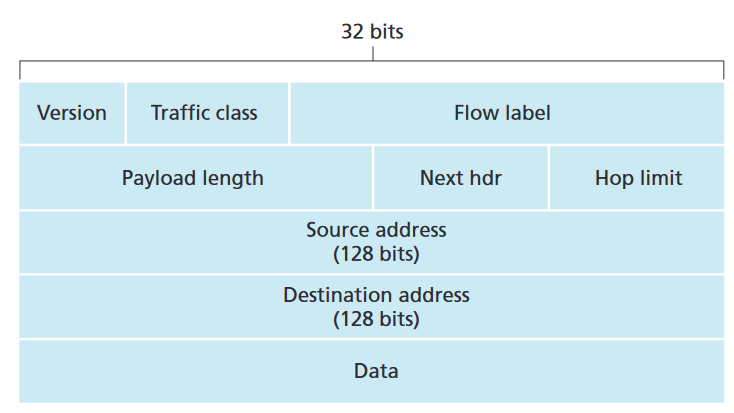
\includegraphics[width=.5\textwidth]{images/ipv6_header.PNG}
\caption{IPv6 Datagram Header}
\label{ipv6_header}
\end{figure}
Functionalities like fragmentation, a header checksum and options were discarded in IPv6. This is mainly due to performance reasons. Not having options makes the header fixed-size and reduces the processing logic. The drawbacks of fragmentation outweighed its benefits. Fragmenting packets was too much of a burden to the routers, in IPv6 the responsibility lies at the end systems to make sure that each IPv6 packet is small enough for every link on the path. The checksum has been discarded because it had to be recomputed on every step which is quite expensive.\vspace{.3cm}\\

IPv6 addresses are denoted in 8 groups of 4 hexadecimal digits separated by colons, where leading zeros are omitted within each group. One consecutive set of groups of zeros can also be omitted. The addresses are also organized hierarchically. The first 48 bits (or more) are the \textbf{routing prefix}, which identifies the responsible ISP. The next 16 bits (or fewer) are the \textbf{subnet ID}. The last 64 bits are the \textbf{interface identifier} and those can be based on the MAC address. An IPv6 host can have multiple addresses at the same interface.
\begin{itemize}
\item \textbf{Link Local:} fe80::/10 (typically fe80::/64)\\
Every host hast this address and it is automatically set up based on the MAC address.
\item \textbf{GUA (global unique address):} currently 2000::/3\\
This address is globally routable and is the \textit{normal} IPv6 address.
\item \textbf{ULA (unique local address):} fc00::/7\\
This address is for local deployments and can be NATed to the GUA.
\end{itemize}


\subsection{Transitioning from IPv4 to IPv6}
The transitioning from IPv4 to IPv6 has been slow and difficult, especially since IPv6 is not backwards compatible. Future systems could be made backwards compatible to support both versions of IP, existing devices however are not able to support the newer version. The replacement of a protocol like this is very difficult if not infeasible. The entire Internet would have to be shut down on a flag day and everything replaced. An alternative approach is \textbf{tunnelling}. Isolated networks that can communicate over IPv6 are connected by routing over IPv4. The IPv6 datagram is encapsulated in a IPv4 datagram and routed to the edge router of the other network.\\
Another option is called \textbf{happy eyeballs}. This approach tries to send both over IPv4 and IPv6 but prefers IPv6. It issues a DNS query for both versions simultaneously. Once the IPv6 address is received, it starts a connection immediately. Ipv4 is a fallback option that is used if the first connection attempt with IPv6 is unsuccessful.


\section{Network Layer - Control Plane}
The \textbf{control plane} of the network layer is the network-wide logic that controls not only how a datagram is forwarded among routers along an end-to-end path from the source host to the destination host, but also how network-layer components and services are configured and managed. Traditionally, control-plane routing protocols have been implemented together with data-plane forwarding functions, monolithically within a router. \textbf{Software defined networking (SDN)} makes a clear separation between the data and control planes, implementing control-plane functions in a separate controller service that is distinct, and remote from the forwarding components of the routers.

\subsection{Routing Algorithms}
The goal of the routing algorithms is to determine good paths from senders to receivers through the network of routers. Good paths are usually the ones with the least cost. The cost of a path can include various factors such as latency, bandwidth, money or number of hops. However, the cost is only concerned with the network topology, not the workload in the network. The union of all shortest paths towards the destination is called a \textbf{sink tree}.\\
There are two different flavours of routing algorithms:
\begin{itemize}
\item \textbf{Centralized} - A centralized routing algorithm computes the shortest path using complete, global knowledge about the network. The algorithm takes as input the network topology, which has to be obtained somehow before the actual computation is performed. The computation itself can be run logically centralized and the result gets distributed or it could be replicated on every routing component. Algorithms that operate on global state information are also referred to as \textbf{link-state (LS) algorithms}. 
\item \textbf{Decentralized} - In a decentralized routing algorithm, the calculation of the shortest path is carried out in an iterative, distributed manner by the routers. No node has complete information about the costs of all network links. Instead, each node begins with only the knowledge of the costs of its own directly attached links. Then the node gradually calculates the shortest paths through an iterative process of calculation and exchange of information with its neighboring nodes. One type of a decentralized routing algorithms are called \textbf{distance-vector (DV) algorithms} because each node maintains a vector of distances to all other nodes in the network.
\end{itemize}

\subsubsection{Distance-Vector Routing}
The distance vector algorithm is iterative, asynchronous, and distributed. Distance-vector routing uses a distributed version of the Bellman-Ford algorithm. Each node maintains a vector of distances to all destinations. Initially, the vector is filled with 0 cost to itself and infinite cost to all other destinations. Each node periodically sends its vector to all of its neighbours. Every round, after receiving the vectors of all neighbours, the node adds the cost of the link to the neighbour's vector for each neighbour respectively. It then sets all vector entries except to itself to the minimum of all received values and sets the corresponding neighbour as the next hop.\vspace{.3cm}\\
One big disadvantage of the distance-vector algorithm is how it reacts to changes in the network. Adding new routes or decreasing link costs does not cause a problem and the new information is propagated very fast through the network. However, if the network is partitioned by failure or a link cost is increased, it can lead to \textbf{routing loops} also known as the \textbf{count-to-infinity} problem. There are two approaches to tackle this problem:
\begin{itemize}
\item \textbf{Poisoned Reverse} - Let there be three nodes $x, y, z$ and $z$ routes to $x$ over $y$. In this case, $z$ will advertise to $y$ that it's distance to $x$ is infinite. This prevents $y$ from trying to route to $x$ over $z$ as long as $z$ routes to $x$ over $y$. Poisoned reverse does not solve the general count-to-infinity problem however. It only prevents two immediately neighbouring nodes from routing in loops, loops involving three or more nodes are still possible.
\item \textbf{Split Horizon} - Split horizon is a less strict version of poison reverse. In split horizon, a host does not send routes to the neighbour it learnt them from.
\end{itemize}
One early protocol to implement distance-vector routing was the \textbf{routing information protocol (RIP)}. The protocol uses hop count as a cost metric and infinity is set at 16 hops, which limited the networks size. It includes split horizon and poison reverse. The protocol runs on top of UDP and vectors are sent every 30 seconds with a 180 second timeout value to detect failures.


\subsubsection{Link-State Routing}
The link-state routing algorithm relies on complete information about the network topology. This is achieved by a \textbf{link-state broadcast} algorithm also referred to as \textbf{flooding}. If a host receives a packet that has to be flooded, it forwards the packet to all of its neighbours. To suppress duplicate messages, the host remembers the message, such that each message is only sent once over each link. This is done by using source and sequence numbers, if a packet is received, only packets with a higher sequence number will be flooded from that point on. \vspace{.3cm}\\

Each node floods a \textbf{link state packet (LSP)} that describes their portion of the topology. Once the information is flooded by each node, every router in the network has knowledge about the complete network topology. The shortest path(s) are then determined using Dijkstra's algorithm, which has a complexity of $\bigo(\log V(V + E))$.\vspace{.3cm}\\

On a change to the network, the updated LSPs are flooded and the routes recomputed. In case of link failure, both nodes notice and send updated LSPs which essentially removes the link from the topology. In case of node failure, all neighbours notice a link has failed. The failed node itself cannot send updated LSPs or update its information. However, according to the fate-sharing principle, this is okay since the node is essentially removed from the network.\vspace{.3cm}\\

Another phenomenon that can appear when using link-state routing is oscillation. If the cost function is based on the traffic on a link. The nodes then recompute the routes, optimizing for low traffic. This results in a switching of routes between paths periodically. One way to reduce the amount of oscillation is to ensure that different nodes compute their routes at different times. To achieve this, nodes flood their LSPs at random intervals.\vspace{.2cm}\\

\begin{figure}
\centering
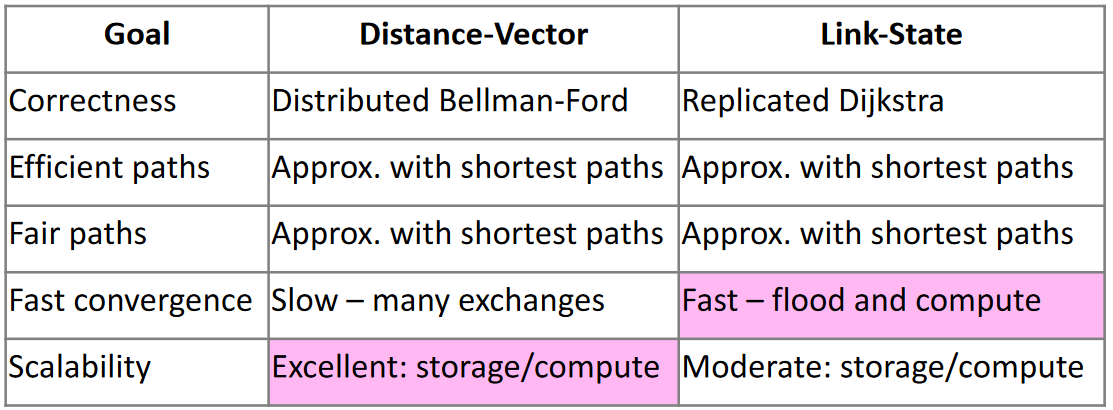
\includegraphics[width=.8\textwidth]{images/dvls.PNG}
\caption{Distance-Vector vs. Link-State}
\label{dvls}
\end{figure}

\subsubsection{Equal-Cost Multipath Routes}
ECMP extends traditional routing to multiple paths. Instead of one shortest path, the set of shortest paths is computed. Since the topology already has redundancy, it might as well be used to improve performance and reliability. Instead of a single next hop is kept for a destination, a set of next hops is remembered.\\
Forwarding with ECMP offers choices on which path a packet is sent. The router could randomly pick a next hop for each packet based on its destination. This balances the load but adds jitter and can cause packet reordering. Another approach is to send packets from a given flow on the same path. This doesn't cause jitter but the traffic is less balanced.

\subsection{Intra-AS Routing in the Internet}
The view of a network as a homogeneous collection of interconnected routers all executing the same routing algorithm is simplistic for two reasons. 
\begin{itemize}
\item Scale - The Internet has become enormous with hundreds of millions of routers. Storing routing information for each possible destination would require enormous amounts of memory. The overhead required to broadcast connectivity and link cost updates among all of the routers would be huge. A distance-vector algorithm that iterated among such a large number of routers would surely never converge.
\item Administrative autonomy - The Internet is a network of ISPs, with each ISP consisting of its own network of routers. An ISP generally desires to operate its network as it pleases or to hide aspects of its network's internal organization from the outside.
\end{itemize}
These problems can be solved by organizing routers into \textbf{autonomous systems (ASs)}, with each AS consisting of a group of rotuers that are under the same administrative control. An autonomous system is identified by its globally unique autonomous system number (ASN), which are assigned by ICANN regional registries. Routers within the same AS all run the same routing algorithm and have information about each other. The routing algorithm running within an autonomous system is called an \textbf{intra-autonomous system routing protocol.}

\subsection{Open Shortest Path First (OSPF)}
OSPF is a link-state protocol that uses flooding of link state information and a Dijkstra's least-cost path algorithm. The algorithm does not mandate how to set link weights, this is up to the network administrator. OSPF advertisements are contained in OSPF messages that are carried directly by IP, with an upper-layer protocol of 89 for OSPF. Therefore, the OSPF protocol must itself implement functionality such as reliable message transfer and link-state broadcast. The OSPF protocol also checks that links are operational via HELLO messages. OSPF also provides the following features:
\begin{itemize}
\item \textbf{Security} - Exchanges between OSPF routers can be authenticated. With authentication, only trusted routers can participate in the OSPF protocol within an AS, thus preventing malicious intruders from injecting incorrect information into router tables. Two types of authentication can be configured, a password-based one and another based on a shared secret authenticated via MD5 hashes.
\item \textbf{Multiple Same-Cost Paths} - OSPF allows multiple paths to be used.
\item \textbf{Integrated support for unicast and multicast routing} - Multicast OSPF provides a simple extension to OSPF to provide for multicast routing.
\item \textbf{Support for Hierarchy} - An autonomous system can be configured hierarchically into areas. Each area runs its own OSPF link-state routing algorithm, with each router in an are broadcastin its link state to all other routers in that area. Within each area, one or more area border routers are responsible for routing packets outside the are. Exactly one OSPF area in the AS is configured to be the backbone are. The primary role of the backbone area is to route traffic between the other areas in the AS. The backbone always contains all area border routers in the AS and may contain internal-routers as well. AS border routers are at the edge of the AS and are responsible for routing traffic to other ASs. The edges of areas lies on area border routers, these routers are part of both the backbone and another area.
\end{itemize}

\subsubsection{Intermediate System to Intermediate System}
This protocol is closely related to OSPF, which was loosely based on IS-IS. IS-IS is also a link-state routing protocol that uses Dijkstra's algorithm to compute the best paths. The network can also be separated into areas.
\begin{figure}
\centering
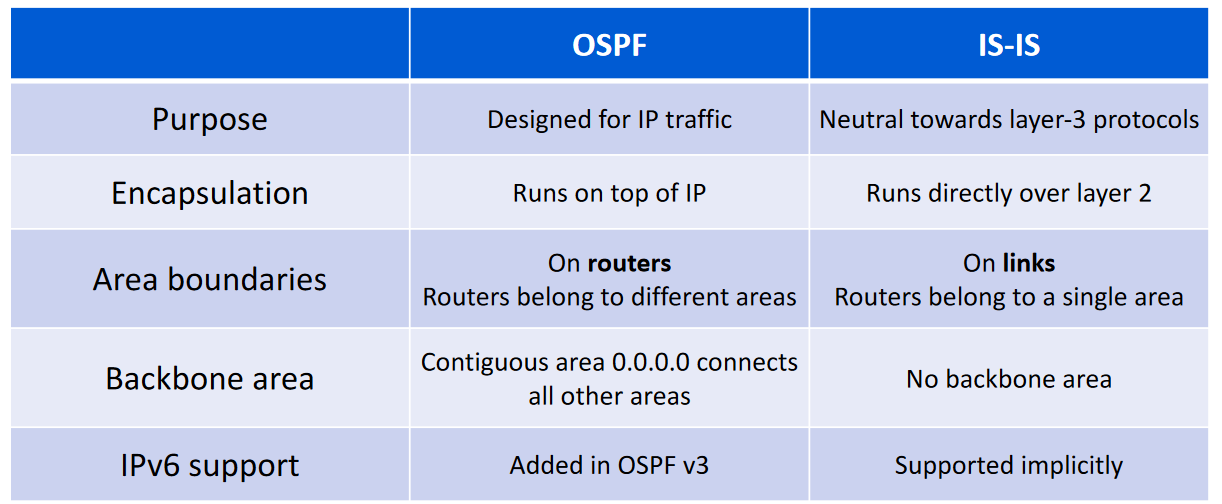
\includegraphics[width=.8\textwidth]{images/ospfvisis.PNG}
\caption{OSPF vs. IS-IS}
\label{ospfvisis}
\end{figure}

\subsection{Routing Among the ISPs}
To route a packet across multiple Ass, we need an \textbf{inter-autonomous system routing protocol}. All the ASs run the same inter-AS routing protocol, called the \textbf{Border Gateway Protocol} known as \textbf{BGP}. BGP is a decentralized and asynchronous protocol like distance-vector routing but it relies on \textbf{path-vector routing} to support flexible routing policies and avoid count-to-infinity.\vspace{.3cm}\\
The role of BGP comes into play when we consider a router inside an AS that wants to forward a packet. For destinations within the AS, the forwarding table is determined by the AS's intra-AS routing protocol. BGP is responsible for routing of packets who's destination is outside of the AS. In BGP, packets are not routed to a specific destination address, but instead to prefixes, with each prefix representing a subnet or a collection of subnets. As an inter-AS routing protocol, BGP provides each router a means to:
\begin{itemize}
\item Obtain prefix reachability information from neighbouring ASs. In particular, BGP allows each subnet to advertise its existence to the rest of the Internet. 
\item Determine the \textit{best} routes to the prefixes. A router may learn about two or more different routes to a specific prefix. To determine the best route, the router will locally run a BGP route-selection procedure using the prefix reachability information it obtained via neighboring routers. The best route will be determined based on policy as well as the reachability information.
\end{itemize}

\subsubsection{Advertising BGP Route Information}
Each router in an AS is either a \textbf{gateway router} or an \textbf{internal router}. A gateway router is a router on the edge of an AS that directly connects to one or more routers in other ASs. An internal router connects only to hosts within its own AS. In BGP, pairs of routers exchange routing information over semi-permanent TCP connections using port 179. Each such TCP connection, along with all the BGP messages sent over the connection, is called a \textbf{BGP connection.} Furthermore, a BGP connection that spans two ASs is called an \textbf{external BGP (eBGP)} connection, and a BGP session between routers in the same AS is called an \textbf{internal BGP (iBGP)} connection.  There is typically one eBGP connection for each link that directly connects gateway routers in different ASs. There are also iBGP connections between routers iwthin each of the ASs. iBGP connections do not always correspond to physical links. In order to propagate the reachability information, both iBGP and eBGP sessions are used.

\subsubsection{Determining the Best Routes}
When a router advertises a prefix across a BGP connection, it includes with the prefix several \textbf{BGP attributes}, the entire announcement is called a \textbf{route}.
\begin{itemize}
\item \textbf{AS-PATH} - The AS-PATH attribute contains the list of ASs through which the advertisement has passed. To generate the AS-PATH value, when a prefix is passed to an AS, the AS adds its autonomous system number (ASN) to the existing list in the AS-PATH. BGP routers also use the AS-PATH attribute to detect and prevent looping advertisements; specifically, if a router sees that its own ASN is contained in the path list, it will reject the advertisements.
\item \textbf{NEXT-HOP} - The NEXT-HOP attribute provides the critical link between the inter-AS and intra-AS routing protocols. The NEXT-HOP is the IP address of the router interface that begins the AS-PATH. 
\end{itemize}
The simplest routing algorithm in BGP is called \textbf{hot potato routing}. In hot potato routing, the route chosen from all possible routes is the route with the least cost to the NEXT-HOP router beginning that route. This method is called hot potato routing because the AS wants to get the packet (the hot potato) out of its own network as fast as possible. The steps for adding an outside-AS prefix in a router's forwarding table for hot potato routing are the following:
\begin{enumerate}
\item Learn from inter-AS protocol that subnet $x$ is reachable via multiple gateways
\item Use routing info from intra-AS protocol to determine costs of least-cost paths to each of the gateways.
\item Hot potato routing: Choose the gateway that has the least cost.
\item Determine from forwarding table the interface $I$ that leads to the least-cost gateway. Enter $(x, I)$ in the forwarding table.
\end{enumerate}
It is important to note that when adding an outside-AS prefix into a forwarding table, both the inter-AS routing protocol (BGP) and the intra-AS routing protocol are used. Hot potato routing is a selfish algorithm because the AS tries to reduce its own cost while ignoring the components of the end-to-end costs outside its AS. It is possible that two routers in the same AS may choose different AS paths to the same prefix and it can lead to asymmetric traffic with each direction taking a different path.\vspace{.3cm}\\
In practice, BGP uses a more complicated algorithm that is more complicated but incorporates hot potato routing. For any given destination prefix, the input into BGP's route-selection algorithm is the set of all routes to that prefix that have been learned and accepted by the router. If there is only one such route, then BGP selects that route. If there are two or more routes to the same prefix, then BGP sequentially invokes the following elimination rules until one route remains.
\begin{enumerate}
\item A route is assigned a \textbf{local preference} value as one of its attributes. The local preference of a route could have been set by the router or could have been learned from another router in the same AS. The value of the local preference attribute is a policy decision that is left entirely up to the AS's network administration. The routes with the highest local preference values are selected.
\item From the remaining routes, the route with the shortest AS-PATH is selected. 
\item From the remaining routes, hot potato routing is used, that is the route with the closest NEXT-HOP router is selected.
\item If more than route still remains, the router uses BGP identifiers to select the route.
\end{enumerate}

\subsubsection{IP-Anycast}
BGP is often used to implement the IP-anycast service, which is commonly used in DNS. IP-anycast is useful to replicate the same content on different servers in many different dispersed geographical locations, having each user access the content from the server that is closest. Each of the servers is assigned the same IP address and standard BGP is used to advertise this IP address from each of the servers. When a BGP router receives multiple route advertisements for this IP address, it treats these advertisements as providing different paths to the same physical location, when in fact, the advertisements are for different paths to different physical locations. When configuring its routing table, each router will locally use the BGP route-selection algorithm to pick the best route to that IP address. One issue that occurs in practice is that because of BGP routing changes, different packets of the same TCP connection can arrive at different instances of the Web server.

\subsubsection{Routing Policy}
The Internet topology is shaped according to business relationships. Autonomous systems only connect if they have a business relationship. There are two main business relationships today:
\begin{itemize}
\item \textbf{Customer/Provider} - Customers pay providers to get Internet connectivity. The amount paid is based on peak usage, usually according to the $95^{\text{th}}$ percentile rule. Every 5 minutes the number of bytes sent or received is counted. At the end of the month all those values are sorted and the top 5\% removed. The highest remaining value is billed.
\item \textbf{Peer/Peer} - Peering ASs don't pay each other for connectivity, they do it out of common interest. 
\end{itemize}
Each AS routes according to its routing policy. To understand the Internet routing, we have to follow the money. Providers transit traffic for their customers but peers do not transit traffic between each other. Customers also do not transit traffic between their providers. Usually, the routing policy follows a simple scheme, where traffic coming from peers is and providers is only propagated to customers.
\begin{figure}[H]
\centering
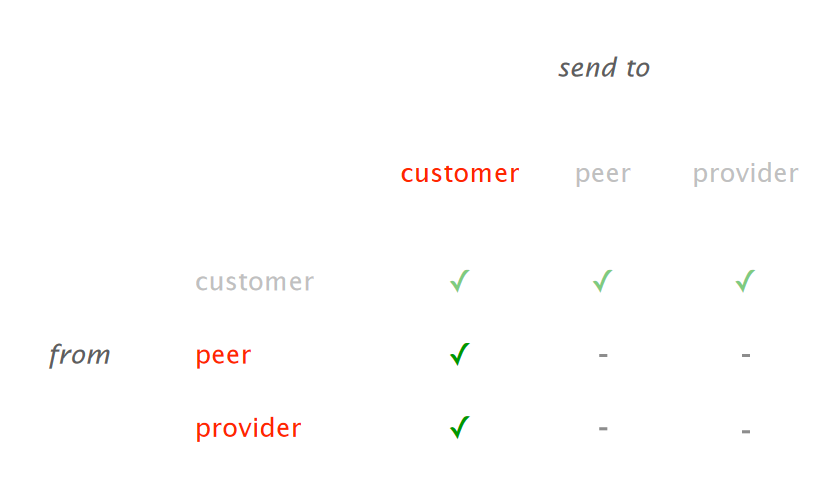
\includegraphics[width=.7\textwidth]{images/policies.PNG}
\caption{Routing Policies}
\label{policies}
\end{figure}
Policies are enforced by constraining which BGP routes are selected and exported. \textbf{Selection} controls the outbound traffic. It chooses which path to use among all paths that were announced to the AS. For a destination, the AS prefers routes coming announced by customers, over routes announced by peers, over routes announced by providers. \textbf{Export} defines which inbound traffic is allowed. An AS might receive a path but choose not to advertise it to other ASs. Other ASs then won't route traffic to a destination over this AS because they don't know there exists a path. \vspace{.3cm}\\

Outbound and inbound traffic can also be controlled to a certain degree using the BGP attributes LOCAL-PREF and MED. LOCAL-PREF is a local attribute (communicated to other internal BGP routers using iBGP) set at the border, it represents how preferred a route is. All routers inside the AS are then going to use the route with the higher local preference. The \textbf{Multi-Exit Discriminator (MED)} is a global attribute (also communicated to other ASs using eBGP) which encodes the relative \textit{proximity} of a prefix to the announcer. In contrast to LOCAL-PREF, a lower MED value indicates closeness is preferred over a higher value. Neighbouring ASs may choose to use the route with the lower MED value, if this does not incur any additional cost for the neighbouring AS. However, if the local preference of another route is higher in the neighbouring AS, it will not care about the announced MED value and chose that route to reduce it's own cost.\vspace{.3cm}\\
The network which is sending the traffic always has the final word when it comes to deciding where to forward. The network which is receiving the traffic can just influence the remote decision, not control it.

\subsection{Internet Control Message Protocol (ICMP)}
ICMP is used by hosts and routers to communicate network-layer information to each other. The most typical use of ICMP is for error reporting. ICMP is not part of IP, but lies just above IP. ICMP messages are carried inside IP datagrams as payload just as TCP or UDP segments. ICMP messages have a type and a code field, and contain the header and the first 8 bytes of the IP datagram that caused the ICMP message to be generated in the first place so that the sender can determine the datagram that caused the error. The following known applications are implemented using ICMP:
\begin{itemize}
\item Ping - The ping program sends an ICMP type 8 code 0 the the specified host. The destination host, seeing the echo request, sends back a type 0 code 0 echo reply.
\item Traceroute - Traceroute sends UDP segments on an uncommon port with increasing TTLs. If the TTL expires at a router, this router sends back an ICMP type 11 code 0 TTL expired to the sender. If a UDP packet makes it to the destination, it is highly likely that no process runs on the given port and the destination sends back an ICMP type 3 code 3 destination port unreachable. The sender then knows that its packets reached the destination.
\end{itemize}
\renewcommand{\arraystretch}{1.4}
\begin{table}[H]
\centering
\begin{tabular}{lll}
\arrayrulecolor{NavyBlue}\hline
ICMP Type & Code & Description \\ \hline
\arrayrulecolor{black}
0 & 0 & echo reply (to ping) \\ \hline
3 & 0 & destination network unreachable \\ \hline
3 & 1 & destination host unreachable \\ \hline
3 & 3 & destination port unreachable \\ \hline
3 & 6 & destination network unknown \\ \hline
3 & 7 & destination host unknown \\ \hline
4 & 0 & source quench (congestion control) \\ \hline
8 & 0 & echo request \\ \hline
9 & 0 & router advertisement \\ \hline
10 & 0 & router discovery \\ \hline
11 & 0 & TTL expired \\ \hline
12 & 0 & IP header bad \\ \hline
\end{tabular}
\end{table}

\section{Link Layer}
The network layer provides a communication service between any two network hosts. Between the two hosts, datagrams travel over a series of communication links. The link layer provides the transmission over these links. There are two fundamentally different types of link-layer channels. The first type are broadcast channels, which connect multiple hosts in wireless LANs, satellite networks, and hybrid fiber-coaxial cable access networks. Since many hosts are connected to the same broadcast communication channel, a so-called \textbf{medium access protocol} is needed to coordinate frame transmission. The second type of link-layer channel is the point-to-point communication link. Coordinating access to a point-to-point link is simpler and managed by a \textbf{Point-to-Point protocol (PPP)}.\vspace{.3cm}\\

When talking about the link-layer we refer to any device as a node, and to interconnects as links. Over a given link, a transmitting node encapsulates the datagram in a \textbf{link-layer frame} and transmits the frame into the link. Although the basic service of any link layer is tot move a datagram from one node to an adjacent node over a single communication link, the details of the provided service can vary from link-layer protocol to the next. Possible services that can be offered by a link-layer protocol include:
\begin{itemize}
\item \textbf{Framing} - Almost all link-layer protocols encapsulate each network-layer datagram within a link-layer frame before transmission over the link. A frame consists of a data field and a number of header fields. The structure of the frame is specified by the link-layer protocol.
\item \textbf{Link Access} - A \textbf{medium access control (MAC)} protocol specifies the rules by which a frame is transmitted onto the link. When multiple nodes share a single broadcast link, the MAC protocol serves to coordinate the frame transmission of the many nodes.\\
\item \textbf{Reliable Delivery} - When a link-layer protocol provides reliable delivery service, it guarantees to move each network-layer datagram across the link without error. Similar to a transport-layer reliable delivery service, a link-layer reliable delivery service can be achieved with acknowledgements and retransmissions. A link-layer reliable delivery service is often used for links that are prone to high error rates, such as a wireless link, with the goal of correcting an error logically on the link where the error occurs rather than forcing an end-to-end retransmission of the data.
\item \textbf{Error Detection and Correction} - The link-layer hardware in a receiving node can incorrectly decide that a bit in a frame is zero when it was transmitted as a one, and vice versa. Such bit errors are introduced by signal attenuation and electromagnetic noise. Because there is no need to forward a datagram that has an error, many link-layer protocols provide a mechanism to detect such bit errors. This is done by having the transmitting node include error-detection bits in the frame, and having the receiving node perform an error check. Error correction is similar to error detection, except that a receiver not only detects when bit errors have occurred in the frame but also determines exactly where in the frame the errors have occurred and then corrects these errors.
\end{itemize}


\subsection{Error-Detection and -Correction Techniques}
Bit-level error detection and correction are two services often provided by the link layer. At the sending node, the data is augmented with \textbf{error-detection and -correction bits (EDC).} Both the data and EDC are sent to the receiving node in a link-level frame. During transmit, both the data and the EDC may be altered. Error-detection and -correction techniques allow the receiver to sometimes, not always, detect that bit errors have occurred and potentially correct them. However, even with the use of error-detection bits there still may be undetected bit errors. As a consequence, the receiver might deliver a corrupted datagram to the network layer. Generally, more sophisticated error-detection and -correction techniques incur a larger overhead. 

\subsubsection{Parity Checks}
The simplest form of error detection is to use a single \textbf{parity bit}. The parity is just the xor of the to be protected data. Every odd number of bit errors can be detected using this method, every even number of bit errors remains undetected.

\subsubsection{Checksums}
In checksumming techniques, the data bits are treated as a sequence of $k$-bit integers. One simple checksumming method is to simply sum these $k$-bit integers and use the resulting sum as the error-detection bits. The \textbf{Internet checksum} is based on this approach, the bytes of data are treated as 16-bit integers and summed using their 1s complement. Carry bits are also readded. The result of the sum is then inverted and put in the segment header. The receiver recalculates the checksum and adds it to the included checksum. If the result is zero, the receiver assumes no errors have occurred.\\
Checksumming methods require relatively little packet overhead but also provide relatively weak protection. Checksumming is mainly used in software, because it is simple and fast to calculate.

\subsubsection{Cyclic Redundancy Check}
CRC codes are also known as \textbf{polynomial codes.} The bit string to be sent is viewed as a polynomial whose coefficients are 0 and 1 values accordingly. CRC codes operate as follows. Consider the $d$-bit piece of data, $D$, to be sent. The sender and receiver agree on a $r+1$ bit pattern, known as the \textbf{generator} $G$. The leftmost bit of $G$ is required to be a one. For the given piece of data $D$, the sender will choose $r$ additional bits, $R$, and append them to $D$ such that the resulting $d + r$ bit pattern is exactly divisible by $G$, i.e. has no remainder using modulo-2 arithmetic. The process of error checking with CRCs is simple: The receiver divides the $d + r$ received bites by $G$. If the remainder is nonzero, the receiver knows that an error has occurred; otherwise the data is accepted as correct. \\
All CRC calculation are done in modulo-2 arithmetic without carries in addition or borrows in subtraction. This means that addition and subtraction are identical, and both are equivalent too the bitwise XOR of the operands. \\
The sender wants to find R such that there is an $n$ such that
\begin{align*}
D \cdot 2^r \; XOR\;R = nG
\end{align*}
If we divide $D \cdot 2^r$ by $G$, the remainder of the result has to be exactly $R$.\vspace{.3cm}\\
A CRC can detect bursts of errors of fewer than $r + 1$ bits. This means all consecutive bit errors of $r$ bits or fewer will be detected. Under appropriate assumptions, a burst of length greater than $r+1$ bits is detected with probability $1 - 0.5^r$. Additionally, the CRC standards can detect any odd number of bit errors.

\subsubsection{Hamming Codes}
The idea of error correction codes is that only a subset of all codewords are correct, a randomly chosen codeword is hence unlikely to be correct. If a codeword is received, it is then mapped to the closest correct codeword. The \textbf{Hamming distance} between two codewords is the number of bit flips required to transform one into the other. The Hamming distance of a code is the minimum hamming distance between any pair of codewords. For a code of Hamming distance $d + 1$, up to $d$ errors will always be detected. For a code of Hamming distance $2d + 1$, up to $d$ errors can be corrected.\vspace{.3cm}\\

The \textbf{Hamming code} gives a method for constructing a code with a Hamming distance of 3. The number of bits needed to achieve this distance is $n = 2^k - k - 1$ where $k$ is the number of check bits.\\
The check bits are put in positions that are power of two, starting with position 1. The check bit at position $p$ is the parity of all positions with a $p$ term in their values. For example, the check bit in position one is the parity bit of all uneven positions, because their value have the rightmost bit set in binary representation, which stands for one.\\
The way to correct an error is outstandingly simple and smart. All parity bits are recomputed, including the check bit. The computed parities are then arranged as a binary number and the value tells the position of the error.

\subsection{Framing}
The packets sent over the link link layer are called frames and are of limited size. However, the physical layer gives the link layer a stream of bits. The link layer has to interpret this sequence as frames. For this, it is important to detect the start and end of a frame in the sequence. 

\subsubsection{Byte Count}
This method supplies every frame with a length field containing the length of the frame. From this, the link layer should be able to deduce the end of the current and the start of the next frame. This approach has an obvious weakness. It is very difficult, if not unfeasible, to re-synchronize once the sender and receiver are desynchronized. Hence, we want to be able to detect the start of each frame.

\subsubsection{Byte Stuffing}
Byte stuffing introduces a special flag byte value that signifies the start or end of the frame. However, this flag value could appear naturally in the frame payload. Therefore, the flag inside the frame has to be \textit{stuffed} with an escape code. Obviously, the special escape code has to be escaped as well. The rules are simple:
\begin{itemize}
\item Replace each FLAG in the data with ESC FLAG
\item Replace each ESC in the data with ESC ESC
\end{itemize}
Any unescaped FLAG marks the start and end of the frame.
\begin{figure}[H]
\centering
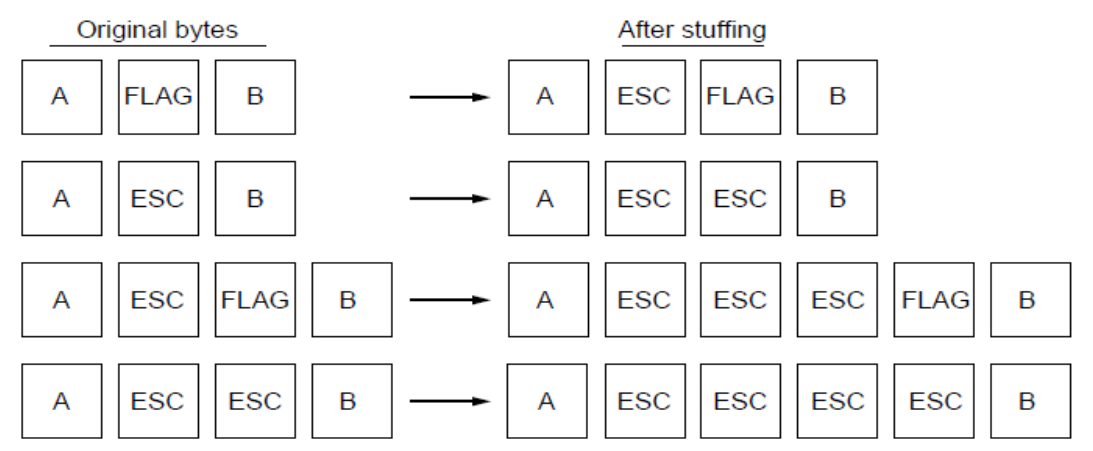
\includegraphics[width=.6\textwidth]{images/byte_stuffing.PNG}
\label{byte_stuffing}
\caption{Byte Stuffing}
\end{figure}

\subsubsection{Bit Stuffing}
The principle of byte stuffing can also be applied at bit level granularity. As an example, we call a flax six consecutive 1s. On transmit, after five 1s in the data, a 0 is inserted. When the receiver sees a 0 after five 1s, this zero is ignored.
\begin{figure}[H]
\centering
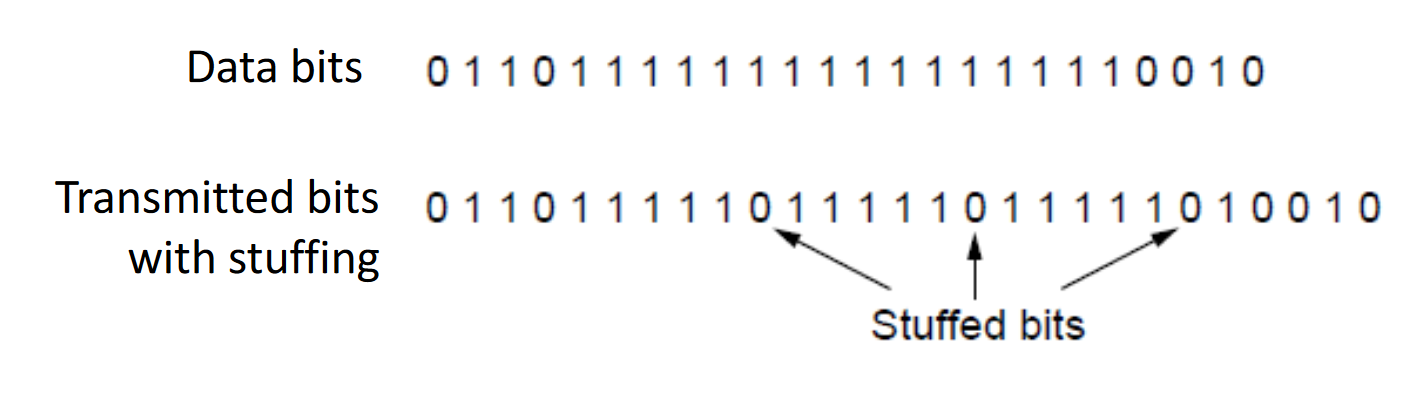
\includegraphics[width=.7\textwidth]{images/bit_stuffing.PNG}
\label{bit_stuffing}
\caption{Bit Stuffing}
\end{figure}


\subsection{Multiple Access Links and Protocols}
There are two types of links, point-to-point links and broadcast links. A point-to-point link consists of a single sender at one end of the link and a single receiver at the other end of the link. A broadcast link can have multiple sending and receiving nodes all connected to the same, shared broadcast channel. The term broadcast is used here because when any node transmits a frame, the channel broadcasts the frame and each of the other nodes receives a copy. A central problem of the link layer is the \textbf{multiple access problem}. It is about how to coordinate the access of multiple sending and receiving nodes to a shared broadcast channel. Computers implement \textbf{multiple access protocols} to regulate their transmission into the shared broadcast channel. Because all nodes are capable of transmitting frames, more than two nodes can transmit the frames at the same time. When this happens, all of the nodes receive multiple frames at the same time; the transmitted frames collide. Typically, when there is a collision, none of the receiving nodes can make any sense of any of the frames that were transmitted. In order to ensure that the broadcast channel performs useful work when multiple nodes are active, it is necessary to somehow coordinate the transmission of the active nodes. We can classify any multiple access protocol as belonging to one of three categories: \textbf{channel partitioning protocols, random access protocols,} and \textbf{taking-turns protocols}.

\subsubsection{Channel Partitioning Protocols}
Time-division multiplexing and frequency-division multiplexing are two techniques that can be used to partition a broadcast channel's bandwidth among all nodes sharing that channel. TDM divides time into time frames and further divides each time frame into time slots. Each time slot is then assigned to one of the attached nodes. Typically, slot sizes are chosen so that a single packet can be transmitted during a slot time. TDM eliminates collision and is perfectly fair, however, it has two major drawbacks. A node is limited to an average bandwidth of $R/N$ (with $R$ being the total bandwidth and $N$ the number of nodes) even when it is the only node with packets to send. A second drawback is that a node must always wait for its turn in the transmission sequence, even if its the only node to send.\\
While TDM shares the broadcast channel in time, FDM divides the $R$ bps channel into different frequencies (each with a bandwidth of $R/N$) and assigns each frequency band to one of the nodes. FDM shares both the advantages and drawbacks of TDM. It avoids collisions and is fair, but also limits a node to a bandwidth of $R/N$ even when it's the only node with packets to send.\\
A third channel partitioning protocol is \textbf{code division multiple access (CDMA)}. CDMA assigns a different code to each node. Each node then uses its unique code to encode the data bits it sends. If the codes are chosen carefully, CMDA networks have the property that different nodes can transmit simultaneously and yet have their respective receivers correctly receive a sender's encoded data bits in spite of interfering transmissions by other nodes.

\subsubsection{Random Access Protocols}
In a random access protocol, a transmitting node always transmits at the full rate of the channel. When there is a collision, each node involved in the collision repeatedly retransmits its frame until its frame gets through without a collision. But when a node experiences a collision, it doesn't necessarily retransmits the frame right away. Instead it waits a random delay before retransmitting the frame. \vspace{.3cm}\\
In the \textbf{slotted ALOHA} protocol, all frames consist of exactly $L$ bits and time is divided into slots of the size $L/R$ seconds (time to transmit one frame). Nodes start to transmit frames only at the beginnings of slots and the nodes are synchronized so that each node knows when a slot begins. If two or more frames collide in a slot, then all the nodes detect the collision event before the slot ends. When a node has a fresh frame to send, it waits until the beginning of the next slot and transmits the entire frame in the slot. If there is no collision, the node is successful in transmitting the frame. If there is a collision, the node detects the collision before the end of the slot. The node retransmits the frame in each subsequent slot with probability $p$ until the frame is transmitted without collision.
This protocol works well under low load, but suffers if the load is high. The efficiency of the slotted ALOHA protocol has a maximum efficiency of 37\% with a large number of hosts. If the time is not slotted, the efficiency is only half as much.\vspace{.3cm}\\

In the ALOHA protocol a node's decision to transmit is made independently of the activity of the other nodes attached to the broadcast channel. The \textbf{carrier sense multiple access (with collision detection (CSMA/CD)} implements two new rules.
\begin{itemize}
\item \textbf{Carrier Sensing} - A node listens to the channel before transmitting. If a frame from another node is currently being transmitted into the channel, a node then waits until it detects no transmission for a short amount of time and then begins transmission.
\item \textbf{Collision Detection} - A transmitting node listens to the channel while it is transmitting. If it detects that another node is transmitting an interfering frame, it stops transmitting and waits a random amount of time before repeating the cycle of sensing and transmitting when idle.
\end{itemize} 
Collisions can still occur, even when carrier sensing is implemented. Imagine two nodes sensing that the channel is unused at the same time and proceeding to transmit their frame. The sensing does not even have to occur simultaneously, since the signal takes time to propagate through the channel. The end-to-end \textbf{channel propagation delay} of a broadcast channel plays a crucial role in determining its performance. The longer this propagation delay, the larger the chance that a carrier-sensing node is not yet able to sense a transaction that has already begun at another node in the network. To be sure that no collision has occurred, a node has to send for two times the channel propagation delay (furthest node starts transmitting just before the signal arrives). To make sure a collision is noticed before the frame is completely transmitted, frames must be big enough such that the frame transmission time is greater than two times the maximal propagation delay. An Ethernet frame must have at least 64 bytes for that reason.\\

The time a node waits after a collision is determined by the \textbf{binary exponential backoff (BEB)} algorithm. When transmitting a frame that has already experienced $n$ collisions, the node chooses a value $K$ from $\{0, 1, 2, ..., 2^{n-1}\}$ at random and waits the chosen amount. For example for Ethernet, the actual amount a node waits is $K \cdot 512$  bit times ($K$ times the amount of time needed to send 512 bits into the Ethernet). It is also to note that each time a node prepares a new frame for transmission, it runs the CSMA/CD algorithm, not taking into account any collisions that may have occurred in the recent past. So it is possible that a node with a new frame will immediately be able to sneak in a successful transmission while several other nodes are in the exponential backoff state.

\subsubsection{Taking-Turns Protocols}
One example of a taking-turns protocol is the \textbf{polling protocol}. The polling protocol requires one of the nodes to be designates as a master node. The master node polls each of the nodes in a round-robin fashion. It allows the nodes to transmit up to some maximum number of frames and moves on to the next. The master node can determine when a node has finished sending its frames by observing the lack of signal on the channel. The polling protocol eliminates the collisions and empty slots that occur in random access protocols. This allows polling to achieve a much higher efficiency. However, it also has a few drawbacks. The polling introduces a polling delay. Another issue is that the master node can fail, if that happens the entire channel becomes inoperative. \vspace{.3cm}\\

A second taking-turns protocol is the \textbf{token-passing protocol}. In this protocol there is no master node. A small, special-purpose frame known as a \textbf{token} is exchanged among the nodes in some fixed order. When a node receives a token, it holds onto the token only if it has some frames to transmit, otherwise it immediately forwards the token to the next node. If a node does have frames to transmit when it receives the token, it sends up to a maximum number of frames and then forwards the token to the next node. Token passing is decentralized and highly efficient. But it has its problems as well. The failure of one node can crash the entire channel. Or if a node accidentally neglects to release the token, then some recovery procedure must be invoked to get the token back in circulation.

\subsection{Switched Local Area Networks}
A local area network that is connected by switches does not use intra-domain routing algorithms like RIP or OSPF to determine paths through the network, since the switches work at the link layer and don't recognize network-layer addresses. Instead of IP addresses, the switches use link-layer addresses to forward link-layer frames through the network of switches.

\subsubsection{Link-Layer Addressing and ARP}
Hosts and routers have link-layer addresses, rather their adapters (network interfaces) do. A host or router with multiple network interfaces will have multiple link-layer addresses associated with it. Link-layer switches owever, do not have link-layer addresses associated with their interfaces. A switch carries the frames between hosts and routers transparently, without the host or router having to explicitly address the frame to the intervening switch. A link-layer address is variously called a \textbf{LAN address,} a \textbf{physical address}, or a \textbf{MAC address}. For most LANs the MAC address is 6 bytes long, giving $2^{48}$ possible MAC addresses. These 6-byte addresses are typically expressed as a pair of hexadecimal numbers, separated by dashes. No two adapters have the same address. The IEEE manages the MAC address space and assigns address spaces to manufacturing companies. When an adapter wants to send a frame to some destination adapter, the sending adapter inserts the destination adapter's MAC address into the frame and then sends the frame into the LAN. Since a switch occasionally broadcasts an incoming frame onto all of its interfaces, an adapter may receive a frame that isn't addressed to it. Thus, when an adapter receives a frame, it will check to see whether the destination MAC address in the frame matches its own MAC address. If there is a match, the adapter extracts the enclosed datagram and passes the datagram up the protocol stack. If there is no match, the adapter discards the frame. However, sometimes a sending adapter does want all the other adapters on the LAN to receive and process the frame it is about to send. In this case, the sending adapter inserts a special MAC \textbf{broadcast address} into the destination address field of the frame. For LANs that use 6-byte addresses, the broadcast address is a string of 48 consecutive 1s (FF-FF-FF-FF-FF-FF).\vspace{.3cm}\\

Because there are both network-layer addresses and link-layer addresses, there is a need to translate between them. For the Internet, this is the job of the \textbf{Address Resolution Protocol (ARP)}. If a node wants to send a frame to another node in the same LAN, it has to give the adapter the destination's MAC address. ARP resolves a destination's IP address to a MAC address for hosts in the same subnet. Each host and router has an \textbf{ARP table} in its memory, which contains mappings of IP addresses to MAC addresses. The ARP table also contains a time-to-live (TTL) value, which indicates when each mapping will be deleted from the table. That table does not necessarily contain an entry for every host and router on the subnet; some may have never been entered into the table, and other may have expired. A typical expiration time is 20 minutes. If a node wants to send a datagram to another node it needs to obtain the destination's MAC address given the IP address. If the ARP table contains this mapping, the task is easy. However, if the ARP table does not currently have an entry for the destination, the sender uses the ARP protocol to resolve the address.\\
First, the sender constructs a special packet called an \textbf{ARP packet}. An ARP packet has several fields, including the sending and receiving IP and MAC addresses. Both ARP query and response packets have the same format. The ARP query packet is encapsulated in a link-layer frame using the MAC broadcast address as the destination and transmitted into the subnet. The frame containing the ARP query is recevied by all the other adapters on the subnet, and each adapter passes the ARP packet within the frame up to its ARP module. Each of thee ARP modules checks to see if its IP address matches the destination address in the ARP packet. The one with a match sends back to the querying host a response ARP packet with the desired mapping. The querying host can then update its ARP table and send its IP datagram, encapsulated in a link-layer frame whose destination MAC is that of the host or router responding to the ARP query.\\
The ARP query message is sent within a broadcast frame, whereas the response ARP message is sent within a unicast frame, since the ARP packet contains all necessary addresses to do this. If the host wants to send a datagram to a host outside of the subnet, it determines the MAC address of the default gateway using ARP.

\subsubsection{Ethernet}
Ethernet is by far teh most prevalent wired LAN technology. The original Ethernet LAN used a coaxial bus to interconnect the nodes. Ethernet with a bus topology is a broadcast LAN, all transmitted frames are received and processed by all adapters connected to the bus.\\
By the late 1990s, most LANs were using a hub-based star topology. In such an installation the hosts and routers are directly connected to a hub with twisted-pair copper wire. A \textbf{hub} is a physical-layer device that acts on individual bits rather than frames. When a bit arrives from one interface, the hub  simply re-creates the bit, boosts its energy strength, and transmits the bit onto all other interfaces. Ethernet with a hub-based topology is also a broadcast LAN.\\
In the early 2000s Ethernet installations continued to use a star topology, but the hub at the center was replaced with a \textbf{switch}. A switch operates at link layer and does only occasionally broadcast the frames to all of its interfaces.\vspace{.3cm}\\

The Ethernet frame consists of six fields:
\begin{itemize}
\item \textbf{Data field} (46 to 1'500 bytes) - This field carries the network-layer datagram. The maximum transmission unit (MTU) of Ethernet is 1'500 bytes. If the datagram exceeds the MTU, the host has to fragment the datagram. The minimum size of the data field is 46 bytes. If the datagram is less than 46 bytes, the data field is padded to 46 bytes. When padding is used, the network layer uses the length field in the IP datagram header to remove the padding.
\item \textbf{Destination address} (6 bytes) - This field contains the MAC address of the destination adapter, or the MAC broadcast address.
\item \textbf{Source address} (6 bytes) - This field contains the MAC address of the adapter that transmits the frame onto the LAN.
\item \textbf{Type field} (2 bytes) - The type field allows Ethernet to multiplex network-layer protocols. A given host may support multiple network-layer protocols. The type field determines, which network-layer protocol the datagram is passed to
\item \textbf{Cyclic redundancy check (CRC)} (4 bytes) - The purpose of the CRC field is to allow the receiving adapter to detect bit errors in the frame.
\item \textbf{Preamble} (8 bytes) - The Ethernet frame begins with an 8-byte preamble field. Each of the first 7 bytes of the preamble has a value of 10101010; the last ybte is 10101011. The first 7 bytes of the preamble serve to \textit{wake up} the receiving adapters and to synchronize their clocks to that of the sender's clock. This is necessary because an adapter will not transmit the frames exactly at the target rate , there will always be some drift form the target rate, which is not known by receiving adapters. The receiving adapter can lock onto the sending adapter's clock by locking onto the bits in the first 7 bytes of the preamble. The last 2 bits of the eight byte preamble are to alert the receiving adapter that the important part is about to come.
\end{itemize}
All of the Ethernet technologies provide a connectionless service to the network layer. There is no handshaking between the adapters. Ethernet technologies provide an unreliable service to the network layer. No positive or negative acknowledgments are sent acknowledgments after the CRC check, in case the check fails, the frame is simply discarded by the receiving adapter. This can lead to gaps in the flow of Ethernet frames. Whether a frame is retransmitted, depends on the used transport-layer protocol.

\subsubsection{Link-Layer Switches}
The role of the switch is to receive incoming link-layer frames and forward them onto outgoing links. The switch itself is transparent to the hosts and routers in the subnet. That is, a host/router addresses a frame to another host/router rather than addressing the frame to the switch and sends the frame into the LAN, unaware that a switch will be receiving the frame and forwarding it. The rate at which frames arrive to any one of the switch's output interfaces may temporarily exceed the link capacity of that interface. To accommodate this problem, switch output interfaces have buffers, like routers.\vspace{.3cm}\\

\textbf{Filtering} is the switch function that determines whether a frame should be forwarded to some interface or should just be dropped. \textbf{Forwarding} is the switch function that determines the interface to which a frame should be directed, and then moves the frame to those interfaces. Switch filtering and forwarding are done with a \textbf{switch table}. The switch table contains entries for some, but not necessarily all  of the hosts and routers on a LAN. An entry in a switch table contains a MAC address, the switch interface that leads toward that MAC address, and the time at which the entry was placed in the table. The switch table is constructed differently to a router's forwarding table. \\
When a frame with destination MAC address $D$ arrives at a switch on interface $x$, the switch indexes its table with the MAC address $D$. There are three possible cases:
\begin{itemize}
\item There is no entry in the table for $D$. The switch forwards copies of the frame to the output buffers preceding all interfaces except for interface $x$. Essentially the switch broadcasts the frame.
\item There is an entry in the table associating $D$ with interface $x$. This means the frame is coming from a LAN segment that contains adapter $D$, hence there is no need to forward the frame and it is discarded.
\item There is an entry in the table, associating $D$ with another interface $y$. In this case, the frame needs to be forwarded to the LAN segment attached to interface $y$. The switch places the frame in the output buffer that precedes interface $y$.
\end{itemize}
A switch has the property that its table is built automatically, dynamically and autonomously without any intervention from a network administrator or from a configuration protocol. Switches are self-learning implementing something called \textbf{backwards learning}. This capability is accomplished as follows:
\begin{enumerate}
\item The switch table is initially empty.
\item For each incoming frame received on an interface, the switch stores in its table the MAC address in the frame's source address field, the interface from which the frame arrived and the current time. Like this, the switch records in its table the LAN segment on which the sender resides.
\item The switch deletes an address in the table if no frames are received with that source address after some period of time (the \textbf{aging time}). 
\end{enumerate}
Because frames are sometimes broadcast the network topology has to be a spanning tree, meaning that there is exactly one path between any two nodes in the network. If there were loops in the network, broadcast frames would be cycled and a switch could have conflicting information about the network topology in its switch table. To ensure that there are no loops in the topology, the switches collectively find a spanning tree. The spanning tree algorithm elects a root node (switch with the lowest address) and grows the tree along the shortest distances from the root. Ports that are not on the spanning tree are turned off and not used. Initially, each switch believes that it is the root of the tree. Then, each switch periodically updates its neighbours with its address, the address of the root and the distance (in hops) to the root. Switches favors ports with shorter distances to lowest root. A swich updates its state if it receives an update that either has a new root (lower address) or a route with lower hops to the current root. The algorithm continuously runs and adapts to state change. Stored information times out and gets updated over time.

\subsubsection{Multi-Protocol Label Switching}
The goal of MPLS is to improve the forwarding speed of IP routers by adopting the key concept from the world of virtual-circuit networks: a fixed-length label. MPLS does not replace IP but rather augments it. Datagrams are forwarded based on the label rather than the IP address whenever possible. The IP datagram is encapsulated in an MPLS header, hence, this is only possible if both devices are MPLS capable. An MPLS-capable router is often referred to as a \textbf{label-switched router}, since it forwards an MPLS frame by looking up the MPLS label in its forwarding table and then passes the datagram to the appropriate interface. To find out if a neighbouring router is MPLS-capable and what label is associated with what IP address, the routers announce available routes and labels to their neighbours. For example, router $R1$ announces that destination $D$ is available with label $x$ to neighbour $R2$. The label distribution is managed by the \textbf{resource reservation protocol (RSVP)}. Since it is possible to have multiple paths in label switching, MPLS allows for traffic engineering.

\subsection{Wireless Links and Network Characteristics}
If we look at a wireless LAN, a wireless network interface would replace the host's wired Ethernet interface, and an access point would replace the Ethernet switch. No changes would be needed at the network layer and above. There are a number of important differences between a wired link and a wireless link.
\begin{itemize}
\item \textbf{Decreasing signal strength} - Electromagnetic radiation attenuates as it passes through matter. Even in free space, the signal will disperse, resulting in a decreased signal strength, sometimes referred to as \textbf{path loss} as the distance between sender and receiver increases. 
\item \textbf{Interference from other sources} - Radio sources transmitting in the same frequency will interfere with each other. In addition to interference from transmitting sources, electromagnetic noise within the environment can result in interference.
\item \textbf{Multipath propagation} - Multipath propagation occurs when portions of the electromagnetic wave reflect off objects on the ground, taking paths of different lengths between a sender and receiver. This results in the blurring of the received signal at the receiver. Moving objects between the sender and receiver can cause multipath propagation to change over time.
\end{itemize}
The receiving host receives an electromagnetic signal that is a combination of a degraded form of the original signal and background noise in the environment. The \textbf{signal-to-noise ratio (SNR)} is a relative measure of the strength of the received signal and this noise. The SNR is typically measured in decibels (dB). The SNR also plays a part in the \textbf{bit error rate (BER)} and the maximum transmission rate of a link.\vspace{.3cm}\\

Another difference between a wired and wireless link is that not all host necessarily hear each other. IN a wired broadcast link, all nodes receive the transmissions from all other nodes. On a wired link, there is the so-called \textbf{hidden-terminal problem}, where two senders that are out of reach from each other or blocked by an obstacle try to send to the same receiver. The signals of both terminals interfere at the receiver, without them knowing about each others transmissions.

\subsubsection{The 802.11 MAC Protocol}
One a wireless device is associated with an \textbf{access point (AP),} it can start sending and receiving data frames to and from the access point. But because multiple wireless devices, or the AP itself may want to transmit frames at the same time over the same channel, a multiple access protocol is needed to coordinate the transmissions. Inspired by the huge success of Ethernet and its random access protocol, the designers of 802.11 chose a random access protocol for 802.11 wireless LANs. This random access protocol is referred to as \textbf{CSMA with collision avoidance (CSMA/CA)}. CSMA stands for \textit{carrier sense multiple access}, meaning that each station senses the channel before transmitting, and refrains from transmitting when the channel is sensed busy. Although Ethernet and 802.11 both use CSMA, the two MAC protocols have important differences. Instead of using collision detection, 802.11 uses collision-avoidance techniques. Additionally, because of the relatively high bit error rates of wireless channels, 802.11 uses a link-layer acknowledgement/retransmission (ARQ) scheme. In the Ethernet MAC protocol, a node listens to the channel as it transmits and aborts if it detects another transmission, this is not done in the 802.11 MAC protocol. There are two important reasons for this:
\begin{itemize}
\item The ability to detect collisions requires the ability to send and receive at the same time. But because the strength of the received signal is typically very small compared to the strength of the transmitted signal at the adapter, it is costly to build hardware that can detect a collision.
\item Even if the adapter could transmit and listen at the same time, the adapter would still not be able to detect all collisions due to the hidden terminal problem.
\end{itemize}
Once a station begins to transmit a frame, that frame is transmitted in its entirety. Because there is a non-negligible chance that his frame may not transmit successfully, 802.11 implements a \textbf{link-layer acknowledgement} scheme. When the destination station receives a frame that passes the CRC, it waits a short period of time known as the \textbf{Short Inter-frame Spacing (SIFS)} and the sends back an acknowledgement frame. If the transmitting station does not receive an acknowledgement within a given amount of time, it assumes that an error has occurred and retransmits the frame using the CSMA/CA protocol t oaccess the channel. IV an acknowledgement is not received after some fixed amount of retransmissions, the transmitting station gives up and discards the frame. \vspace{.3cm}\\

Assuming a station has a frame to transmit, it follows the 802.11 CSMA/CA protocol doing the following steps:
\begin{enumerate}
\item If initially the station senses the channel idle, it transmits the frame after a short period of time known as the \textbf{Distributed Inter-frame Space (DIFS)}.
\item Otherwise, the station chooses a random backoff value using binary exponential backoff and counts down this value after DIFS when the channel is sensed idle. While the channel is sensed busy, the counter remains frozen.
\item When the counter reaches zero, the station transmits the entire frame and then waits for an acknowledgement.
\item If an acknowledgement is received, the transmitting station knows that its frame has been correclty received at the destination station. If the station has another frame to send, it begins the CSMA/CA protocol at step 1 (I assume in the book they say step 2 but this doesn't make a lot of sense). If the acknowledgement isn't received, the transmitting station reenters the backoff phase in step 2, with the random value chosen from a larger interval.
\end{enumerate}
The 802.11 MAC protocol also includes a nifty (but optional) reservation scheme that helps avoid collisions even in the presence of hidden terminals. In order to avoid the hidden terminal problem, the IEEE 802.11 protocol allows a station to use a short \textbf{Request to Send (RTS)} control frame and a short \textbf{Clear to Send (CTS)} control frame to reserve access to the channel. When a sender wants to send a data frame, it can first send an RTS frame to the AP, indicating that the total time required to transmit the data frame and the acknowledgement frame. When the RTS frame is received by the AP, it gives the sender explicit permission to send and also instructs the other stations not to send for the reserved duration.

\section{Physical Layer}
The physical layer is concerned with how signal are used to transfer message bits over a link. The wires or other physical media carry analog signals, what we want to send are digital bits. In an abstracted model of the physical link, the link is defined by its properties such as the transmission rate or the latency. There are also other important properties such as whether the channel is broadcast and which type of error model it uses (e.g. whether bits are lost or changed by). When talking about data rates or data sizes, we adopt the notion of base 10 for rates and base 2 for data sizes. For example, $ 1 Mbps = 1'000'000 bps$ but $1 KB = 2^{10} bytes$. \\
The \textbf{latency}, or delay, is the time needed to send a message over a link. The latency is composed of two separate delays:
\begin{itemize}
\item \textbf{Transmission delay} - Time to push the $M$ bits of a message onto the link with rate $R$.\\
$L_{trans} = M/R$
\item \textbf{Propagation delay} - Time for the bits to propagate across the link.\\
$L_{prop} = length/\text{speed of signal}$
\end{itemize}
The overall latency is usually dominated by either of the two. The maximum amount of data that can be in-flight at any given point in time is given by the \textbf{bandwidth-delay product.}

\subsection{Frequency Representation}
A signal over time can be represented by its frequency components. Basically, a signal can be deconstructed into their frequencies by the Fourier analysis. The higher frequency components of the signals get attenuated more strongly than lower frequencies during the transmission. This can lead to the loss of the higher frequency components. This is important because the sharp edges of a digital signal are represented using the higher frequencies. Additionally to attenuation, noise is added to the signal.

\subsection{Modulation}
Modulation is the process of translating the digital data into an analog signal. The simplest modulation method is called \textbf{Non-Return to Zero (NRZ)} where a 1 is represented by a high voltage and a 0 is represented by a low voltage. This is a bad method because electricity flows. Another issue is counting repeated bits. If the clocks of sender and receiver are slightly out of sync the receiver may miscount the number of repeated bits.\vspace{.3cm}\\

The \textbf{Manchester Coding} addresses this problem, it represents a 1 by a transition from a high voltage to a low voltage and a 0 by a transition from a low voltage to a high voltage or vice versa. Because there is a transition for every single bit transmitted, it is easy to synchronize the clocks on the go. However, because the transition has to happen in the middle of the cycle, the sender essentially needs to essentially double the frequency which is kind of wasteful. \vspace{.3cm}\\

Another way to tackle clock recovery is called \textbf{4B/5B}. It maps every 4 data bits into 5 code bits without long runs of zeros. In such a code word there are at most 3 zeros. Additionally, the signal is inverted (a transition) on a 1 to prevent long runs of 1s. This is called \textbf{Non-Return to Zero with Inversion (NRZI)}. \vspace{.3cm}\\

\textbf{Passband Modulation} does not send the signal directly to the wire like \textbf{baseband modulation}, which we have seen so far. This is because in baseband modulation we need higher frequencies which don't travel well on fiber or wireless. Passband modulation carries a signal by modulating a carrier. The carrier is simply an oscillating signal at a desired frequency that is resistant to noise and attenuation. This carrier is then modulated by changing the amplitude, frequency or phase.\\
\begin{itemize}
\item In \textbf{amplitude shift keying} the bits are encoded by changing the amplitude of the carrier.
\item In \textbf{frequency shift keying} the bits are encoded by changing the frequency of the carrier.
\item In \textbf{Phase shift keying} the bits are encoded by changing the phase of the carrier.
\end{itemize}
These methods also allow to encode different levels of alteration, which allow for the transmission of multiple bits at the same time. Additionally, it is also possible to use multiple of these modulation methods simultaneously.

\subsection{Fundamental Limits}
Given a channel with bandwidth $B$, signal strength $S$, and noise strength $N$. $B$ limits the rate of of transitions. $S$ and $N$ limit how many signal levels we can distinguish.\vspace{.3cm}\\

The Nyquist limit states that the maximum symbol rate is $2B$ if the receiver can receive at a bandwidth of $B$. Thus if there are $V$ signal levels, ignoring the noise, the maximum bit rate is $R = 2B \log_2 V$ bits/sec.\vspace{.3cm}\\

The amount of signal levels that can be distinguished also depends on $S/N$, or the \textbf{signal-to-noise ratio (SNR)}. The SNR given on a logarithmic scale in deciBels can be computed as $SNR_{dB} = 10 \log_{10}(S/N)$. The \textbf{Shannon limit} is for capacity $C$, the maximum information carrying rate of the channel:
\begin{align*}
C = B \log_2(1 + S/N) \text{bits/sec}
\end{align*}

\section{Networking Algorithms}

\subsection{Shortest Path Algorithm} 
Shortest path algorithms are applied to weighted graphs to find the path between a source node and a destination node such that the sum of the weights on the path  is minimal. Different types of graphs require different algorithms:
\begin{itemize}
\item Dijkstra's algorithm is used for graphs with non-negative weights. The time complexity with a binary heap is $\bigo ((|V| + |E|)\log|
V|))$.
\item (Distributed) Bellman-Ford can be used for all graphs that do not contain negative cycles. The time complexity is $\bigo (|V| \cdot |E|)$.
\item Breadth-first search (BFS) can be used in case of unweighted graphs and runs in time complexity $\bigo (|V| + |E|)$.
\end{itemize}
Typical criteria for a cost function in networking are latency, bandwidth, or loss rate. However, all of these algorithms assume that the edge cost is additive, which is not the case for all of these criteria.
\begin{itemize}
\item Latency
\begin{itemize}
\item Latency somewhat corresponds to the length of the link and therefore is an additive property. Hence, the algorithms above can minimize for latency.
\end{itemize}
\item Loss rate
\begin{itemize}
\item Loss rate is not additive but multiplicative.
\item Weights can be transformed to an additive quantity by applying the logarithm.
\end{itemize}
\item Bandwidth
\begin{itemize}
\item The bandwidth of a path is the minimum among all the edges
\item Still fulfills the important \textbf{isotonicity property}. Given two paths $P_1$ and $P_2$ from $A \to B$ and a path $P_3$ from $B \to C$. If $P_1$ is better than $P_2$, then the extended path $P_1 + P_3$ is at least as good as $P_2 + P_3$.
\item This allows the application of modified shortest-path algorithms that use the minimum instead of the sum as the operation when extending paths.
\end{itemize}
\end{itemize}
However, as soon as we start combining multiple of those criteria, we violate the isotonicity property.
\begin{itemize}
\item \textbf{Shortest widest path}
\begin{itemize}
\item Optimize for bandwidth ($w$) first
\item Among all paths of maximum bandwidth, select the one of minimal length $(l)$
\item Lexicographic order for $(w, -l)$.
\end{itemize}
\item \textbf{Widest shortest path}
\begin{itemize}
\item Optimize for length first, bandwidth second
\item Lexicographic order for $(-l, w)$.
\end{itemize}
\end{itemize}

\subsection{Traffic Engineering}
Traffic engineering is concerned with flow problems in networks. Given a network, how much traffic can flow from the source to the destination. This problem is called the \textbf{maximum-flow problem}. Max-flow goes hand in hand with the min-cut, since they have equal values. The maximum flow represents, how much traffic a network can carry. The minimal cut is a metric for how reliable a network is. The Ford-Fulkerson algorithm finds the maximum flow as long as the edge capacities are integers. The runtime of Ford-Fulkerson is $\bigo (mnU)$ where $U$ is the maximal edge capacity. The Edmonds-Karp algorithm is an optimized version that guarantees termination, even when edge capacities are not integers, and the time complexity is $\bigo (|V|^2 \cdot |E|)$.\vspace{.3cm}\\

These algorithms can also be used to solve problems where there are multiple sources and destinations in the network. This is done by introducing a new, single source that has edges of infinite capacity to all sources in the original network. Analogously, a new, single destination is introduced. However, the problem changes completely, when the flow from one source has to end in a specific destination. This problem is called the \textbf{Multi-commodity flow (MCF)} problem and it cannot be solved using the standard algorithms.\vspace{.3cm}\\

Another problem relevant for traffic engineering is the \textbf{maximum matching problem}. This problem is concerned with finding the maximum set of edges, such that no vertex is covered by two edges. In computer networks this could appear when searching for the maximum number of simultaneous circuits or in the switching fabric of an optical fiber switch. This problem can be solved either as a flow problem with Edmonds-Karp algorithm or with the \textbf{Hopcroft-Karp} algorithm in $\bigo((|V| + |E|)\cdot \sqrt{|V|})$.


\subsection{Linear Programming}
Linear programming is a general technique developed for linear optimization problems under some constraints. A linear program consist of \textbf{variables, an objective and, constraints.} Variables are values that can change during the optimization problem, such as the flow on an edge. The objective function $\theta$ is must be a linear combination of variables that is going to be optimized. The constraints are also a linear combination of variables that are enforced during the optimization.\\
The \textbf{canonical form} of a linear program contains only the following things:
\begin{itemize}
\item Vector of variables: $x = (x_1, ..., x_n)^T, x \geq 0$
\item Objective: maximize $\theta = c^T \cdot x$, where $c = (c_1, ..., c_n)^T$.
\item Constraints: $A \cdot x \leq b$, where $A = (a_{ij})$ is an $m \times n$ matrix and $b = (b_1, ..., b_m)^T$.\\
$A, b, c$ are parameters that do not change during the optimization process.
\end{itemize}
The canonical form only allows the maximization of the objective, less-or-equal constraints and variables greater or equal to zero. Every linear program can be converted into the canonical form. \vspace{.3cm}\\

There already exist various algorithms for solving linear programs, that take any linear program in canonical form. Their runtime is $\bigo (n^3)$ as a rule of thumb, the best current complexity just about $\bigo (n^{2.05})$. Typically, linear programs are much slower to solve than specialized algorithms for the problems. However, many problems can be expressed in linear programs and they are much easier to develop than a specialized algorithm. Furthermore, efficient linear program solvers are widely available and ready to use. Lastly, linear programs can often be easily adopted for variations of a problem, where the specialized algorithm might completely fail.

\subsubsection{Linear Program for Max-Flow}
The maximum flow problem and the multi-commodity flow problem can be solved using the linear programs in \autoref{table:flow}. Linear programming is the best known solution for MCF. It is to note, that there are multiple possible objectives to optimize in the case of MCF such as
\begin{itemize}
\item Maximize the sum of flows of all commodities.
\item Maximize minimum of all commodities.
\item Define demand for each commodity and maximize average \textit{fulfillment ratio}.
\end{itemize}
\begin{table}[H]
\centering
\begin{tabular}{|l|l|l|}\hline
{\color{NavyBlue} Variables} & \tabitem Flow $S \to T: f$ & \tabitem Flow from commodity $\alpha$ $S_\alpha \to T_\alpha: f_\alpha$ \\
& \tabitem Flow on edge $u \to v: f_{uv}$ & \tabitem Flow for commodity $\alpha$ on edge $u \to v: f_{\alpha, uv}$ \\ \hline
{\color{NavyBlue} Objective} & maximize $f$ & maximize $\sum_\alpha f_\alpha$ \\ \hline
{\color{NavyBlue} Notation} & $F(v) = \sum_{w \in E^+(v)} f_{vw} - \sum_{u \in E^-(v)} f_{uv}$ & $F_\alpha(v) = \sum_{w \in E^+(v)} f_{\alpha, vw} - \sum_{u \in E^-(v)} f_{\alpha, uv}$ \\ \hline
{\color{NavyBlue} Constraints} & 1. Edge capacities: $\forall u \to v \in E:$ & 1. Edge capacities: $\forall u \to v \in E:$ \\
& \quad \tabitem $0 \leq f_{uv}$ & \quad \tabitem $0 \leq f_{\alpha, uv}$ \\
& \quad \tabitem $f_{uv} \leq c_{uv}$ & \quad \tabitem $\sum_\alpha f_{\alpha, uv} \leq c_{uv}$ \\
& 2. Flow from $S : f = F(S)$ & 2. Flow from $S_\alpha : f_\alpha = F_\alpha(S_\alpha)$ \\
& 3. Flow conservation: & 3. Flow conservation: \\
& \quad $\forall v \in V \backslash \{S, T\} : F(v) = 0$ & \quad $\forall \alpha, \forall v \in V \setminus \{S_\alpha, T_\alpha\}: F_\alpha (v) = 0$ \\ \hline
\end{tabular}
\caption{Flow Linear Programs}
\label{table:flow}
\end{table}

\subsubsection{Linear Program for Shortest Path}
The shortest path problem can be solved by linear programs in two different ways.
\begin{table}[H]
\centering
\begin{tabular}{|l|l|l|}\hline
{\color{NavyBlue} Variables} & Is edge $u \to v$ on SP? $x_{uv}$ & Distance $S \to u: \: d_u$ \\ \hline 
{\color{NavyBlue} Objective} & minimize $\sum_{u \to v \in E} x_{uv} \cdot w_{uv}$ & maximize $d_T$ \\ \hline
{\color{NavyBlue} Notation } & $X(V) = \sum_{w \in E^+(v)} x_{vw} - \sum{u \in E^-(v)} x_{uv}$ & \\ \hline
{\color{NavyBlue} Constraints} & 1. Path $S \to T$ is connected: & $\forall u\to v \in E:\; d_v \leq d_u + w_{uv}$ \\
& \quad $\forall v \in V \setminus \{S, T\}:\: X(v) = 0$ & \\
& 2. Path starts at $S:\:X(S) = 1$ &  \\
& 3. $0 \leq x \leq 1$ & \\ \hline
\end{tabular}
\end{table}
If multiple shortest paths exist, the pseudo-flow may be distributed among these multiple shortest paths.

\subsubsection{Integer Linear Programming}
Integer linear programming is a variation of standard linear programming where variable are restricted to integer values. The problem with this is that the general space of integer linear programs is \textbf{NP hard}. However, this does not mean that every integer linear program is hard, many of them can be solved efficiently.

\section{Probabilistic Techniques}

\subsection{Load Balancing}
To ensure availability and increase performance, often resources are replicated on a number of servers. \textbf{Load balancing} refers to techniques to distribute the requests such that the response time is kept uniformly low and the load on the servers is uniform as well.\\
One possible way to distribute the requests is in \textbf{round-robin} fashion, where the load balancer sequentially cycles through the servers. However, this approach can lead to imbalances if the requests follow a pattern (e.g. every $n$-th request is significantly more work). It also gets more complicated if there are multiple load balancers.\\
A second approach could be to query or track the server load and send requests to the server that experiences the least load. But this introduces overhead for querying or tracking. Furthermore, if multiple load balancers are in operation, they will all send their requests to the server with the least load, leading to a spike in workload.\vspace{.3cm}\\

A third approach is to pick a server uniformly at random. We ask ourselves the question; how often does imbalance occur? This load balancing behavior can be modeled by the \textbf{balls into bins problem}, where the balls are the requests and the bins are the servers. Assuming we want to put $m$ balls into $n$ bins, we experience the following probabilities:
\begin{itemize}
\item Probability that ball $i$ and $j$ land in the same bin: $\frac{1}{n}$
\item Expected number of collisions: $\frac{1}{n} \cdot m \choose 2 = \frac{m(m-1)}{2n}$
\item Number of balls that will cause this expectation to exceed 1: $\sqrt{2n}$
\end{itemize}
When we try to put $n$ balls into $n$ bins, the expected \textbf{maximum} load on any bin is $\bigo (\frac{\log n}{\log \log n}$.\\
We can improve this by picking two random bins instead of one. Then, the load of both bins is queried and the less loaded one is picked. This reduces the expected maximum load of one bin to $\bigo ( \frac{\log \log n}{\log 2})$. In general if we make $k$ choices, the behavior is $\bigo (\frac{\log \log n}{\log k}$. \vspace{.3cm}\\

\subsubsection{Hashing}
Sometimes only a single request is sent to the server, like in DNS for example. However, often the client and server exchange multiple messages. Fully random load balancing causes problems if packets of the same session are directed to different servers. Therefore, we may want to randomize over sessions or flows. In IPv6 for example we can randomize over flow identifiers, but what about IPv4? There we can use hash functions, which are assumed to be uniformly random. For example, we can take the hash over source and destination IP addresses, ports and the protocol. The request is then assigned to a server based on this hash value.\vspace{.3cm}\\

Because the hash function is deterministic, we run into problems when a server fails. In that case we have to somehow redefine the mapping. But by doing so, most sessions will be reassigned, which is not favorable. The solution to this problem is \textbf{consistent hashing}. Consistent hashing interprets the image space of the hash function as a circle, i.e. connecting highest and lowest address. Each server identifier, is hashed into this image space. A request is assigned to the server, whose hashed identifier succeeds the hash of the request parameters. One issue with this naive implementation is that in case of failure, all the load the failed server is assigned to a single server, which essentially doubles its load. To improve failover behavior, each server is given multiple server identifiers that are hashed into the image space. In case of failure, the load is now distributed among multiple servers.

\subsection{Membership Testing}
Given some object and a set of objects, we want to determine, whether that object is contained in the set. A simple way to achieve this is to use a hash table. Every object that is in the set gets hashed and its value in the hash table set to true. When the membership of an object is tested, that object is hashed and it is checked if the value is true. In case the value is false, we can be sure that the object is not part of the set, since the hash function is deterministic. If the value is true, we cannot quite be certain because of hash collisions, there is a possibility for false positives. Many applications can live with false positives as long as the probability is low enough, the probability can be reduced by increasing the size of the hash table. \vspace{.3cm}\\

Another way to decrease the probability of false positives is by using \textbf{bloom filters}. Bloom filters use multiple hash functions instead of just one. A general bloom filter has a bit vector $V$ of $m$ bits, initially all set to zero. When an element is inserted, the value of $k$ hash functions is computed and the corresponding bit in $V$ is set to true for all of them. To test if an element has already been seen, we evaluate the hash functions and check if all bits are set. If this is the case, we say the element has been seen, otherwise it is new. \\
A bloom filter where $n$ elements are inserted, the bit vector $V$ is of length $m$ and there are $k$ hash functions, the following probabilities are experienced:
\begin{itemize}
\item Probability that $V[i] = 0$ after $n$ insertions: $(1 - \frac{1}{m})^kn \approx e^{-\frac{kn}{m}}$
\item False-positive rate (Given an item not in the set, the probability to predict it to be in the set): $P[FP] \approx (1 - e^{\frac{-kn}{m}})^k$
\end{itemize}
As we can see the false-positive rate depends on the number of hash functions $k$. The value of $k$ that minimizes the false positive rate is $k \approx \frac{m}{n}ln 2$. The minimized false-positive rate is $P[FP] \approx 2^{-\frac{m}{n}ln2}$.\vspace{.3cm}\\

In practice, we also have the problem that the number of elements to be inserted is not limited. This means the bloom filter fills up over time. One approach would be to empty the filter periodically, accepting that we lose all memory of the last objects. This leads to false negatives as well. A way to fight the \textit{memory loss} is to use a primary and a secondary filter. Elements are only inserted into the primary filter. Testing for membership happens on both filters. Periodically, the primary and secondary filter are swapped. False negatives are still possible with this approach, but since we don't lose all entries at once, those have to lie further back in time. In applications like caches this is not a problem, since elements are not kept in the cache forever anyway. Cache filtering is an approach to avoid single requests from filling the cache. An element is only loaded into the cache if it has been accessed for the second time in given time period.

\subsection{Traffic Monitoring}
Traffic monitoring is motivated is used to detect anomalies or to better manage the network. For example, to detect DoS attacks, enforce quality of service, account for usage-based pricing, or for traffic engineering to better balance load. Traffic monitoring can be done at different granularities, for example at flow level. Some applications might also only be interested in parts of the header fields such as only the source/destination address. The difficulty of traffic monitoring is the sheer amount of traffic. Core routers in the Internet forward multiple terabits of traffic per second. There are around 20 million different flows on a 1 Tbps router.\\
Probabilistic traffic monitoring allows for a tradeoff between accuracy and efficiency. It can reduce the overhead of monitoring but delivers less accurate results. The challenge is to give results that are good estimates with a high probability given limited memory and processing resources.

\subsubsection{Sampled Netflow}
Standard Netflow samples every packet, sampled Netflow only samples every $k$-th packet. For each flow entry, a tuple $\{C_{pkt}, C_{byte}\}$ is kept and updated with every sampled packet. The recorded is then multiplied by $k$ to get an estimate of the actual traffic. This method can both under- and overestimate the size of a flow. The estimate is very imprecise for short lived flows.\vspace{.3cm}\\

The problem with general-purpose flow measurements is that it is either imprecise or unfeasible. The solution is to focus only on specific traffic information such as
\begin{itemize}
\item \textbf{Large Flows}
\item Subpopulations (small-volume flows)
\item \textbf{Number of flows}
\item Address access patterns
\item Per-source behavior of small flows
\item Flow distribution
\end{itemize}

\subsubsection{Large-Flow Detectors}
A large flow is a flow that consumes more of the link capacity than a given threshold during a given measurement interval. For example, flows that take more than 1\% of link capacity. To monitor this is reasonable since a small portion of flows makes up a large portion of the traffic. It is possible to efficiently identify large flows because the number of large flows is significantly smaller than the total number of flows. We will look at three types of large-flow detectors:
\begin{itemize}
\item Sampling-based
\item Sketch-based
\item Eviction-based
\end{itemize}

The \textbf{sampling-based} system uses the \textbf{sample-and-hold} algorithm that uses a byte-sampling technique. Instead of sampling every $k$-th packet like Netflow, each byte is sampled with a probability $p$. Practically, a packet of length $s$ is sampled with probability $1-(1-p)^2$. Once a packet from a flow is sampled, every subsequent packet from that flow is also sampled and the flow metrics updated. The flows that are being sampled are likely to be the large flows. Since we sample every packet of a given flow, no flow will be overestimated. Underestimation is still possible since the starting packets of the flow may be missed.\vspace{.3cm}\\

The \textbf{sketch-based} system uses a multistage filter. A single filter is practically a counting bloom filter with a single hash function. On an incoming packet, flow ID is hashed and the counter in the filter updated. A flow is considered large if the counter value in the associated counter is above some given threshold. To reduce the false-positive probability of multiple small flows contributing to the same counter, multiple filters are used. A flow is then considered large if the corresponding counter values in all filters are above some threshold.\vspace{.3cm}\\

The \textbf{eviction-based} system implements algorithms to find frequent items. Frequent items are those whose frequency are above a given threshold $\vartheta$. The majority algorithm is an exact, linear-time algorithm that finds frequent items in two passes with $\frac{1}{\vartheta}$ space.\\
The goal is to find all items that appear in a stream of $m$ items more than $k$ times with no false negatives. The algorithm uses $n = m/k - 1$ labeled counters. For each new item the following case distinction is made:
\begin{itemize}
\item If there is a counter with the label of the new item, increase the counter.
\item If there is a counter that is zero, set the label to the new item and increase to 1.
\item Else, all counters are decremented.
\end{itemize}
The labels at the end are candidates for items that occur more than $k$ times. The second pass is required to make sure for which candidate items this is the case. Since in traffic monitoring we cannot afford to store all packets for the second pass. There is the EARDet algorithm that is a modification to the majority algorithm that does not require the second pass.

\subsubsection{Number of Flow Estimation}
The simplest idea to estimate the number of flows is just to record all distinct flow IDs in a set and count them. However, this is unfeasible since the number of flows is too big to keep a record for every distinct flow. A more reasonable approach is to use bloom filters and increase a counter if the incoming packet belongs to a new flow. \vspace{.3cm}\\

An approach to probabilistic counting could look as follows. Each flow ID is used to generate a value in [0, 1). A single counter is then associated with the smallest recorded value $v$. The number of flows can then be estimated using $v$, under the assumption that the hash values are going to be uniformly distributed. Since this method has very large variance, it is better to keep track of the $k$ smallest values and use those for the estimation.

\section{Video Streaming and Content Distribution Networks}


\subsection{Internet Video}
In streaming stored video applications, the underlying medium is prerecorded video. These prerecorded videos are placed on servers, and users send request to those servers to view the videos on demand. \\
A video is a sequence of images, typically being displayed at a constant rate, such as 24 or 30 images per second. An uncompressed, digitally encoded image consist of an array of pixels, with each pixel encoded into a number of bits to represent luminance and color. A video can be compressed, trading off video quality  with bit rate. Today's compression algorithms can compress a video to essentially any bit rate desired. We can also use compression to create multiple versions of the same video, each at a different quality level. Users can then decide which version they want to watch as a function of their current available bandwidth.

\subsection{HTTP Streaming and DASH}
In HTTP streaming, the video is simply stored at an HTTP server as an ordinary file with a specific URL. When a user wants to see the video, the client issues a GET request for that URL. The server then sends the video file within an HTTP response message, as quickly as the network allows it. ON the client side, the bytes are collected in an application buffer. Once the number of bytes in this buffer exceeds a threshold, the client application begins the playback. \\
This method, although widely deployed, has significant drawbacks. For example, all clients receive the same encoding of the video, despite the large variations in the amount of bandwidth available to a client, both across different clients and also over time for the same client. This has led to the development of \textbf{Dynamic Adaptive Streaming over HTTP (DASH).} In DASH, the video is encoded into several different versions with respective bit rates. The HTTP server stores URLs and bit rates of each version in a \textbf{manifest file}. The client first requests the manifest file and learns about the versions. The client then dynamically requests chunks of video segments of a few seconds in length. While downloading a segment, it observes the experienced throughput. Based on the perceived throughput and how full the buffer is, the client application adapts its choice for the next segment of the video. Making a choice based on the buffer is called \textbf{buffer-based adaptation.}

\subsection{Content Distribution Networks (CDN)}
Content distribution networks take on the challenge to distribute massive amounts of data to users around the world. A CDN manages servers in multiple, geographically distributed locations. A user request will then be served by the closest server cluster of the CDN. A CDN is is favorable over a single data center for several reasons:
\begin{itemize}
\item A single data center presents a single point of failure.
\item Improves end-to-end delay and potentially throughput because the clusters are located closer to the user.
\item A single data center is inefficient and more expensive from a network perspective since the same traffic travels over the same links multiple times.
\end{itemize}
There are both \textbf{private and third-party CDNs}. A private CDN is owned and managed by the content provider, while a third-party CDN distributes content on behalf of multiple content providers. Esentially, there are two different server placement philosophies:
\begin{itemize}
\item \textbf{Enter Deep} - The server clusters are deployed in access ISPs all over the world. The result is that the clusters are very close to the user, thereby improving user-perceived delay and throughput. But because of this highly distributed design, the task of maintaining and managing the cluster becomes challenging.
\item \textbf{Bring Home} - This philosophy envisions fewer, larger server clusters. Instead of getting inside the access ISPs, these clusters are placed at Internet exchange points (IXPs). This design typically results in lower maintenance and management overhead, possibly at the expense of higher delay and lower throughput to end users.
\end{itemize}
Once the clusters are in place, the CDN replicates content across its clusters. However, not every cluster should replicate all of the content, since some content rarely viewed in some parts of the world. Instead, many CDNs operate more as a cache. When a client requests a resource from a cluster that is not storing the resource, the cluster retrieves the resource from a central repository or from another cluster and stores a copy locally while transmitting the resource to the client simultaneously. Once the storage of the cluster becomes full, it removes resources that are not frequently requested. \vspace{.3cm}

Somehow the CDN has to select a cluster to which a user is redirected. There are two approaches to this:
\begin{itemize}
\item \textbf{DNS-based} - When a client wants to access content on the CDN, he submits a DNS query to his local DNS server. This LDNS then performs an iterative query, at some point this query is going to reach the authoritative name server of the CDN. This authoritative name server is then going to guess the location of the client, based on the IP address of his local DNS server. Depending on this location, the authoritative DNS server is then going to return a suitable IP address of one of its server clusters. Additionally, the DNS server could take into account the load on the clusters. To allow dynamic changes, the TTL is set low to prevent caching. This method grants very high control over the distribution of request. However, it is fairly complicated and it has another weakness. A user might choose a distant name server as its LDNS, which  results in suboptimal behavior.
\item \textbf{BGP-Anycast-based} - This method lets BGP do the work. All server clusters are announced under the same prefix. BGP is treating those multiple announcements as multiple possible paths to the same physical location, when in fact they are different paths to different physical locations. BGP is then going to route the traffic to the closest cluster from its perspective. This method is simpler but doesn't allow for the same precise control as the DNS-based approach. Additionally, it takes longer for the path to adjust in case of changes.
\end{itemize}

\section{Routing Security}
\begin{itemize}
\item \textbf{Secrecy} - Keep data hidden from unintended receivers
\item \textbf{Confidentiality} - Keep someone else's data secret
\item \textbf{Privacy} - Keep data about a person secret
\item \textbf{Anonymity} - Keep the identity of a protocol participant secret
\item \textbf{Data Integrity} - Ensure data is correct. Prevents unauthorized changes
\item \textbf{Entity Authentication/Identification} - Verify the identity of another protocol participant
\item \textbf{Data authentication} - Ensure that data originates from claimed sender
\end{itemize}
\begin{figure}[H]
\centering
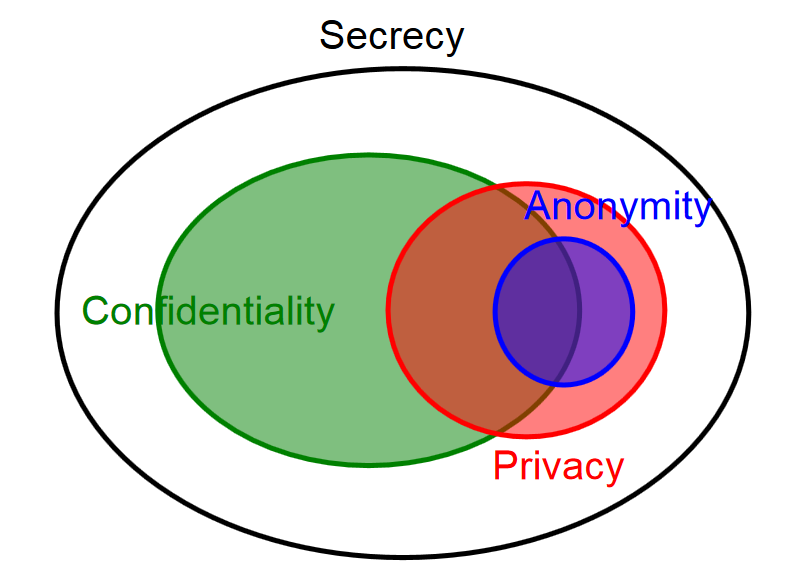
\includegraphics[width=.4\textwidth]{images/secrecy.PNG}
\label{secrecy}
\caption{Secrecy}
\end{figure}

\subsection{Intra-Domain Routing}
To perform an attack on link-state routing, the adversary has to compromise one router or one routing adjacency. Most of the attacks on intra-domain routing aim at performing Denial-of-Service (DoS) or intercept traffic.
\begin{itemize}
\item Interception
\begin{itemize}
\item The attacker can eavesdrop on, drop, modify, inject, and delay traffic by steering the traffic along paths controlled by the attacker. This can be done by flooding bogus announcements. Research has shown that any forwarding tree can be achieved through malicious OSPF messages.
\end{itemize}
\item Denial-of-Service
\begin{itemize}
\item The attacker can induce churn to overload the routers by announcing and withdrawing at a very fast pace, so the routers have to constantly recompute.
\item The attacker floods the routers' link-state database by injecting thousands of prefixes.
\item Induce congestion and increase the delay by steering the traffic along fewer and lower-throughput paths.
\item It is even possible to make nodes completely unreachable by steering the traffic along black holes or loops.
\end{itemize}
\end{itemize}
All those attacks are possible because advertisements can be injected by anyone and legitimate advertisements can be altered. The solution would be to use cryptographic authentication. Each announcement would have to be authenticated and the topology information cryptographically protected. For example, a node should only be able to announce prefixes that actually belong to its subnet.

\subsection{Inter-Domain Routing}
BGP has a severe lack of security, this can be seen in the following attack vectors.

\subsubsection{Prefix Hijacking}
IP address blocks are assigned to ISPs by the regional internet registries. The AS who owns this prefix then announces that prefix or this is done by its upstream providers on its behalf. However, nothing is stopping another AS to announce the same prefix. Since BGP does not verify that the AS is authorized to do so, any AS can originate said prefix. It is also hard to verify that such an announcement is malicious, since registries of prefix ownership are inaccurate and there are legitimate use cases to announce a prefix in different ASs. Once the prefix is announced, the BGP routing algorithm redirects the traffic to the closest AS that announced the prefix, just like in BGP anycast. This means that some traffic is going to the malicious AS. The malicious AS has two options for the redirected traffic:
\begin{itemize}
\item \textbf{Blackhole} - The traffic is dropped
\item \textbf{Snooping} - The traffic is inspected and redirected back to the legitimate AS
\end{itemize}
Prefix hijacking is hard to debug, since the victim AS doesn't really see the problem, since the route might not get announced to it. Additionally, the prefix hijack does not necessarily incur a loss of connectivity. In the case of snooping, all the traffic still reaches the legitimate AS, be it with higher delay. Even in case of blackholing, the traffic is only redirected for a subset of sources. Prefix hijacking can be diagnosed by analyzing BGP updates from many vantage points.

\subsubsection{Sub-Prefix Hijacking}
This type of attack announces a more specific prefix than the victim AS. Since the route is more specific, every other AS is going to redirect its traffic towards the malicious AS. \\
A common adversary that uses this attack are spammers. Since the spammers send lots of emails, the IP addresses from which the spam originates get put on blacklists. Hence, it is smarter to not use ones own IP  addresses. The solution is quite obvious, the spammers hijack someone's address space and use that for the spam. In case this address block lands on a blacklist, the spammers just hijack the next block and the entity who owns the address space has the issues.

\subsubsection{BGP Route Poisoning}
ASs have a lot of different options and motivations to announce incorrect paths. In one scenario, the AS 701 wants to attract traffic from sources that would normally try to avoid AS 3715, or it wants to make AS 88 look closer to the Internet's core. In that case, AS 701 can announce the path \textit{AS 701 88}. This essentially removes AS 3715 from the path.
\begin{figure}[H]
\centering
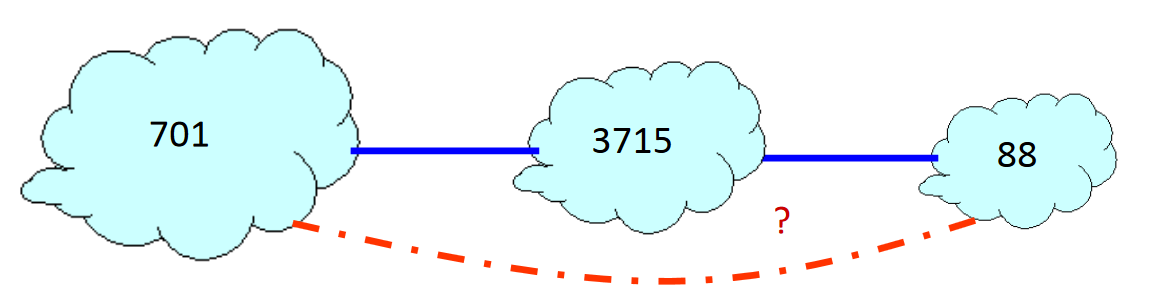
\includegraphics[width=.6\textwidth]{images/remove_AS.PNG}
\caption{Remove AS}
\label{remove_AS}
\end{figure}

An AS might also want to add an AS to the route. This can be used to control the incoming traffic. Let's say AS 701 is connected directly to AS 88 but does not want to route traffic from AS 3715 to AS 88. Instead of announcing the route \textit{AS 701 88} it announces the route \textit{AS 701 3715 88}. If AS 3715 receives this route, it is going to trigger its loop detection. This makes AS 3715 not send route traffic to AS 88 over AS 701, thinking it would already get routed over itself.
\begin{figure}[H]
\centering
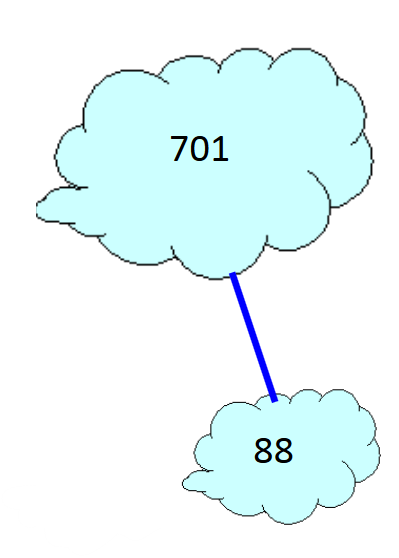
\includegraphics[width=.3\textwidth]{images/add_AS.PNG}
\caption{Add AS}
\label{add_as}
\end{figure}

An AS could also add hops at the end of the path. This helps evade detection for a bogus route by adding the legitimate AS to the end. For example, AS 701 announces \textit{AS 701 88 3} instead of \textit{AS 701 88}.
\begin{figure}[H]
\centering
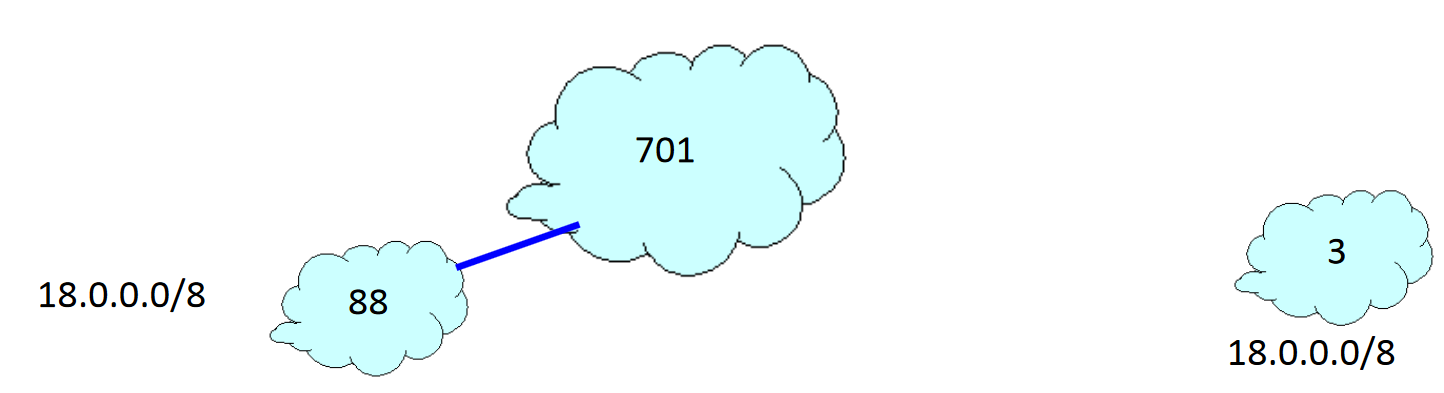
\includegraphics[width=.8\textwidth]{images/add_hop.PNG}
\label{add_hop}
\caption{Add Hop}
\end{figure}

\subsubsection{BGPsec}
BGPsec is a more secure version of BGP that proposes enhancements. BGPsec uses a \textbf{Resource Public-Key Infrastructure (RPKI)} that provides per-prefix certificates. This enables the signature of the first-hop AS, which is called \textbf{Route Origin Authorization (ROA)}. With origin authentication and cryptographic signatures it is possible to prevent the aforementioned route poisoning attacks.\\
The AS that owns the prefix, announces the prefix and cryptographically signs it using its private key. Any 
AS that reannounces the prefix, then adds its own signature while maintaining all the older signatures as well. The AS that receives a route can then go through the list of signatures and verify them. Like this it is not possible to add any other AS to the route, since one would have to sign it. It is also not possible to remove an AS from the route, since the AS that announces the prefix, inludes the AS number it is going to announce the prefix to. Further, it is not possible to announce a prefix that one does not own, since the owner of the prefix has a special certificate for this which is checked through a delegation chain from ICANN. This \textbf{address attestation} is referred to as ROA. \vspace{.3cm}\\

Even with these enhancements BGPsec has quite a few challenges. In order for BGPsec to work, there has to be an accurate, and reachable registry of prefix owners. This becomes incredibly hard to maintain, especially with ownership changes. Additionally, this kind of public-key infrastructure creates a circular dependency. For the verification of routes, the registry of prefix owners has to be reachable, but for the registry to be reachable, the routing already has to work. The task of verifying becomes increasingly difficult if not every AS implements the enhancements. Because some routes will still be accepted without signatures, the AS has to check if an announcement has been made with correct ROA information. Further, these changes introduce an overhead which lowers performance and increases the time of convergence. \\
With not all of the enhancements of BGPsec currently implemented, a lot of AS implement heuristics to detect suspicious routes. For example, an AS could look at
\begin{itemize}
\item Which AS usually announces a prefix
\item Never before seen subpaths
\item Out-of-Band detection mechanisms
\item Delay the adoption of unfamiliar routes when possible
\item Prefer routes that agree with the past
\end{itemize}

BGP cannot only be attacked on the control plane by route poisoning and prefix hijacking but also on the data plane. Even when traffic is forwarded on an advertised path, a malicious AS or router within an AS must not comply with this route. It can send the traffic wherever it wants since the route is not enforced. The malicious router could then drop packets, or only drop specific traffic, or even just slow down some traffic. To avoid detection, the malicious router can handle debugging traffic such as traceroutes different and just forward them along the legitimate path.


\section{DNS Security}
The DNS system can be attacked in various ways. For the following examples, we're going to use a simplified architecture that is globally distributed, scalable and ideally has no single point of failure.
\begin{figure}[H]
\centering
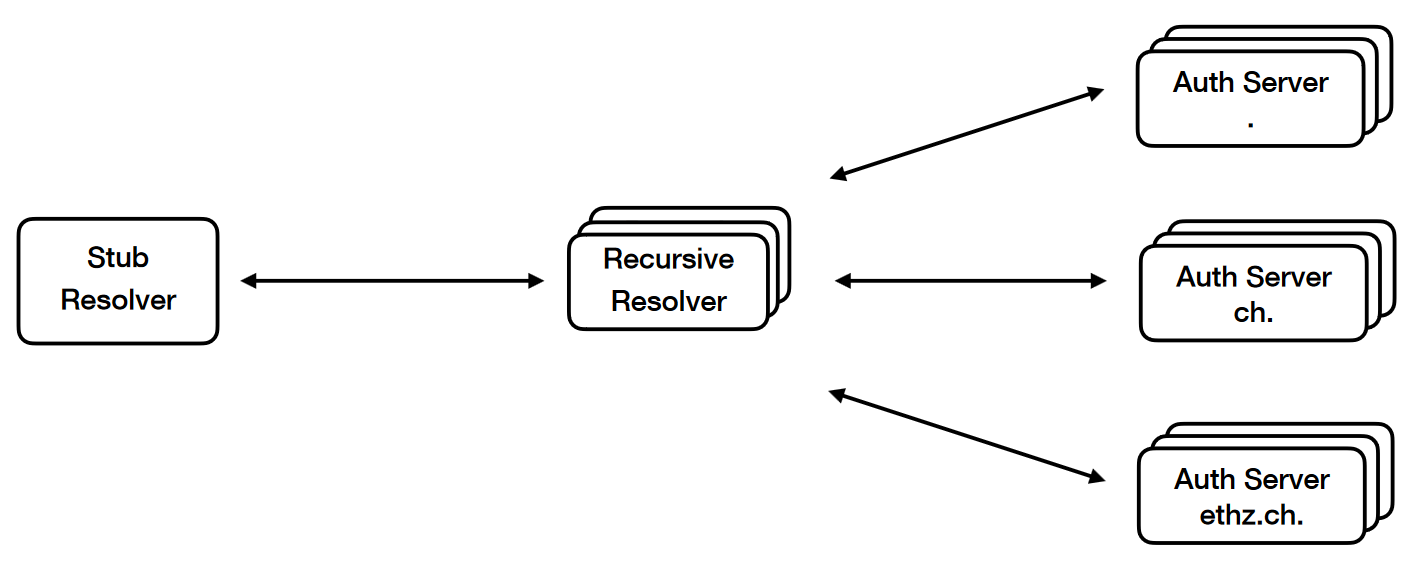
\includegraphics[width=.8\textwidth]{images/dns_architecture.PNG}
\label{dns_architecture}
\caption{Simplified DNS Architecture}
\end{figure}
The DNS system servers as a tool or is target for three different attack types:
\begin{itemize}
\item Denial of Service (DoS) - as tool and target
\item Privacy Leakage
\item DNS data spoofing
\end{itemize}

\subsection{DoS with \& against DNS}
In a naive DoS attack, the attacker just tries to send as much traffic as possible to the victim. The victim however will most likely be able to handle the traffic of a single or a few sources. Therefore, the attacker uses two core principles of DoS attacks, \textbf{reflection and amplification.} Reflection is the process of causing a remote system that is not necessarily attacker controlled to send traffic to the victim. This can be done by \textbf{IP spoofing} where the attacker sends packets under the victims address as source address and hence the returning traffic gets routed to the victim. \textbf{Amplification} happens when the response is larger than the request. Say the response to a DNS query is double the size, this means the \textbf{amplification factor} is two. With these two principles combined, the attacker can send many small queries to a lot of powerful servers, which send large response messages to the victim.

\subsubsection{Water Torture - Random Prefix Attacks}
In this attack, the victim is a name server which is the authoritative name server of say \textit{victim.com}. The attacker sends a lot of DNS queries for random prefixes of \textit{victim.com}, for which records are unlikely to exist. The random prefixes are necessary because otherwise the recursive resolver would just cache the responses, reducing the load on the victim. This attack method has no amplification factor, however, if the attacker controls a big number of hosts (e.g. in a botnet), it can still generate a significant amount of traffic.
\begin{figure}[H]
\centering
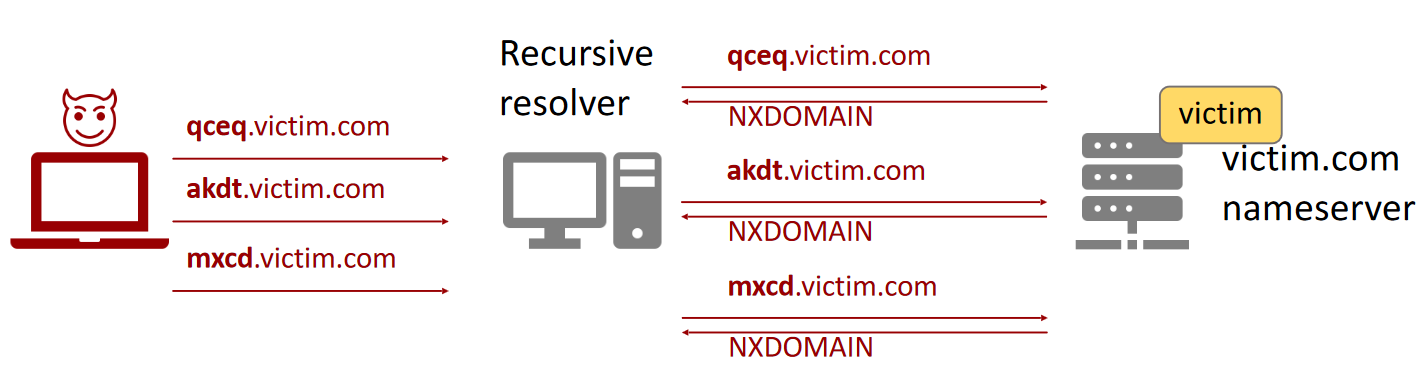
\includegraphics[width=.7\textwidth]{images/water_torture.PNG}
\label{water_torture}
\caption{Water Torture Attack}
\end{figure}

\subsubsection{Indefinitely Delegating Nameserver (iDNS)}
In this attack, the attacker controls a client and a name server, which is the authoritative name server of say \textbf{attacker.com}. The victim is the recursive resolver. This name server stores an indefinitely long chain of NS records without glue records. This results in the name server delegating the recursive resolver to new subzones. The recursive resolver is going to stop the process at some point but empirical evidence shows that the amplification factor is above 10.
\begin{figure}[H]
\centering
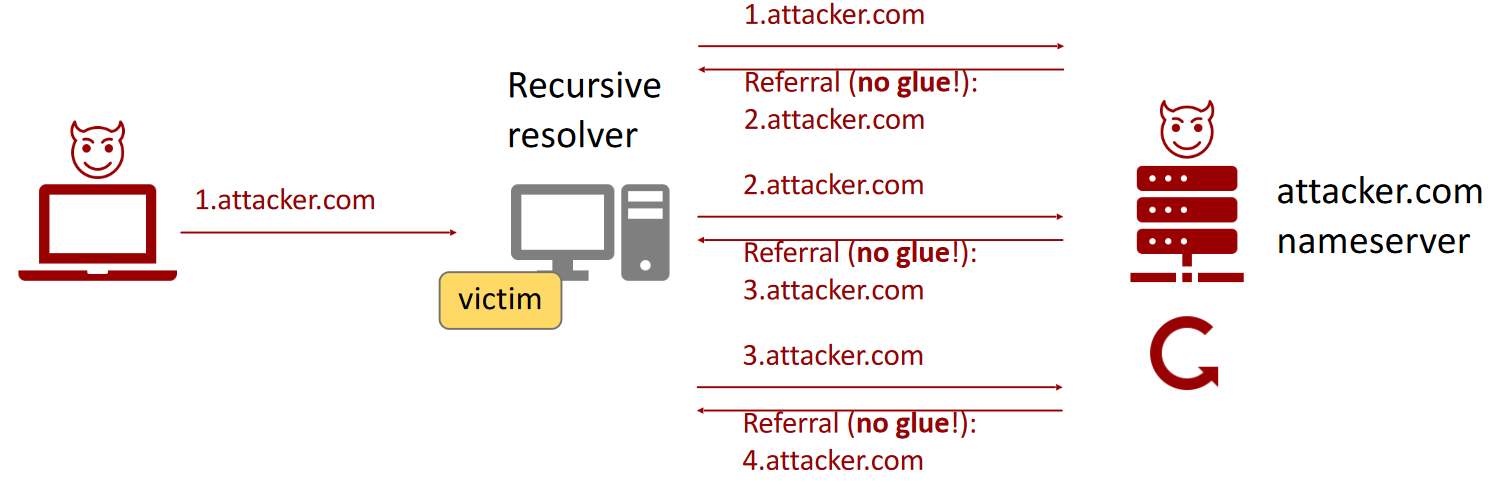
\includegraphics[width=.7\textwidth]{images/idns.PNG}
\caption{iDNS}
\label{idns}
\end{figure}

\subsubsection{DNS Unchained}
In this attack, the attacker controls a host and is able to add DNS records in a shared nameserver that is the victim. Additionally, another name server is needed. The idea is to let the recursive resolver bounce between the two name servers by adding respective CNAME records. If the TTL is set to zero in the victim name server and very high in the auxiliary name server, the load is mainly hitting the victim because the recursive resolver caches the responses from the auxiliary name server. How long the recursive resolver is going to follow the spiel is implementation dependent but empirical evidence suggests an amplification factor above 8.5.
\begin{figure}[H]
\centering
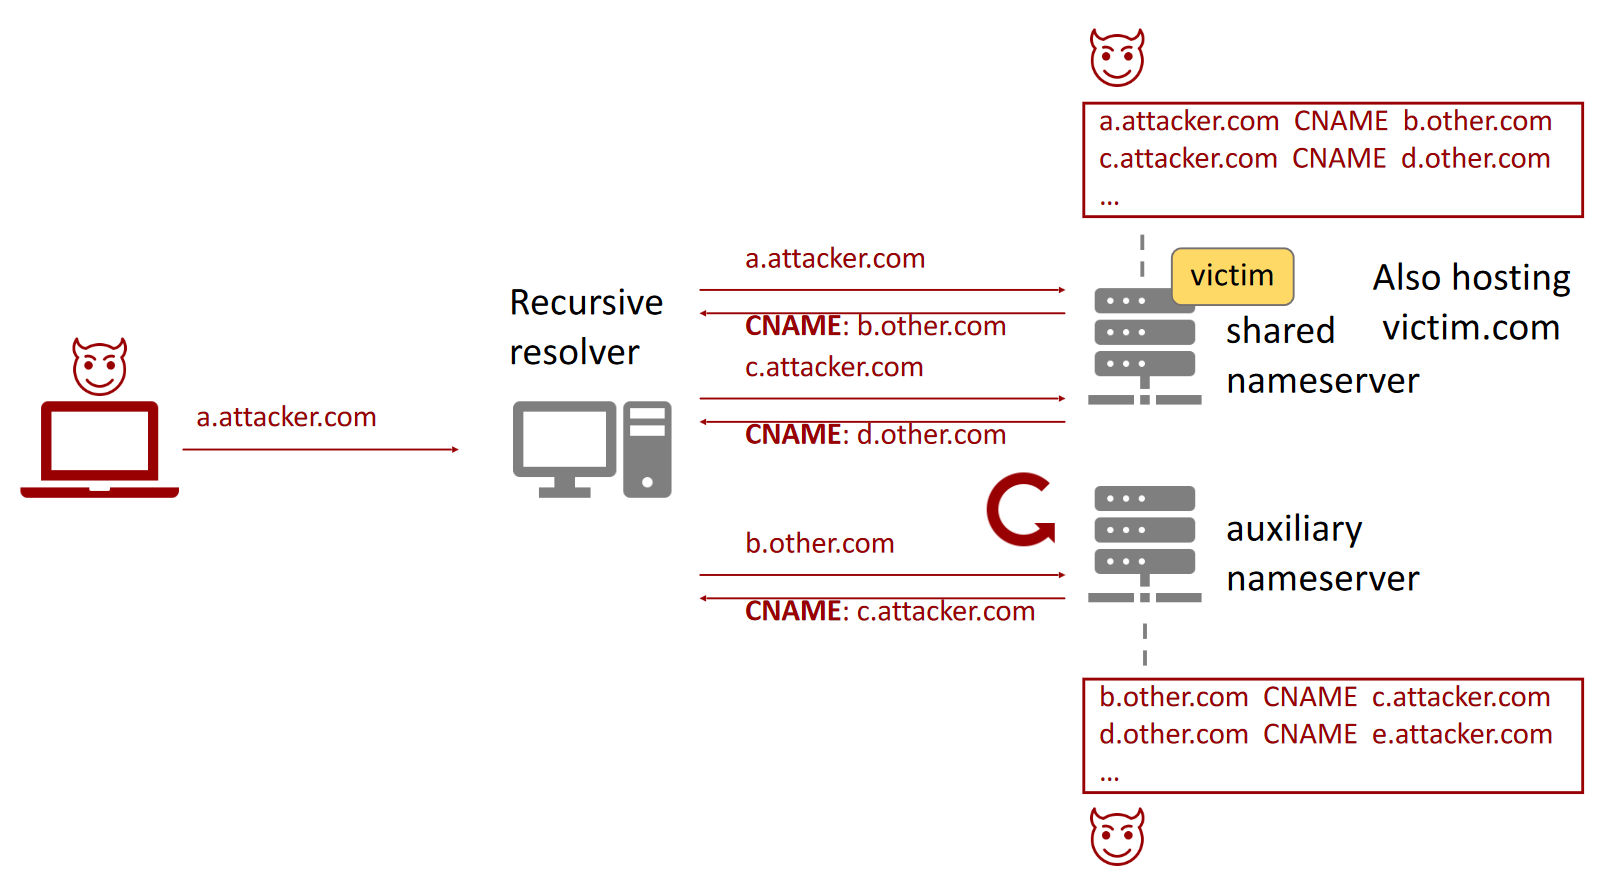
\includegraphics[width=.7\textwidth]{images/unchained.PNG}
\caption{DNS Unchained}
\label{unchained}
\end{figure}

\subsubsection{NXNS Attack}
This attack exploits the aggressive behavior of recursive resolvers in the case that many referral NS records without glue records are received. Because the recursive resolver does not know which of the given name servers is the fastest, it aggressively creates parallel subqueries. This attack can be directed at the recursive resolver and or the victim nameserver. The resolver is attacked by sending many requests for potentially different domains. The victim name server is attacked by using many resolvers. The amplification factor of this attack can exceed 1000.
\begin{figure}[H]
\centering
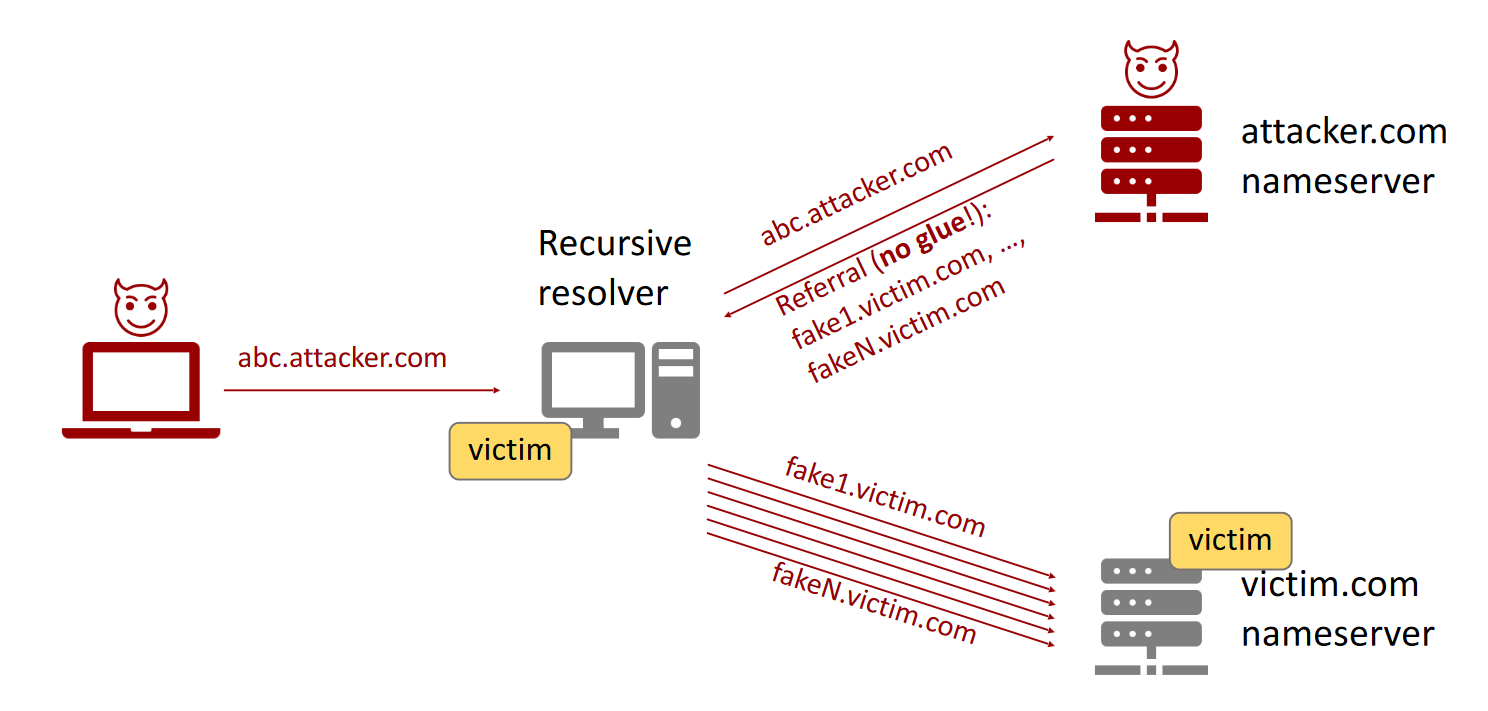
\includegraphics[width=.7\textwidth]{images/nxns.PNG}
\caption{NXNS Attack}
\label{nxns}
\end{figure}

\subsection{DNS Privacy}
Obviously, DNS is a public service and is storing no sensitive or personal data. However, the requests shouldn't be public since they reveal the browsing history of a user. When using standard DNS, every name server on the path knows the entire request, even if it does not need the entire knowledge to provide it's service.

\subsubsection{DNS Query Minimization}
DNS Qmin tries to only reveal the necessary information. It sends only the TLD to the root server and so on. 
One issue of DNS Qmin appears when the prefixes are extremely long and all point to the same authoritative name server. This causes the recursive resolver to generate a lot more messages than if the entire domain was sent to the authoritative name server. This is a new DoS attac vector.
\begin{figure}[H]
\centering
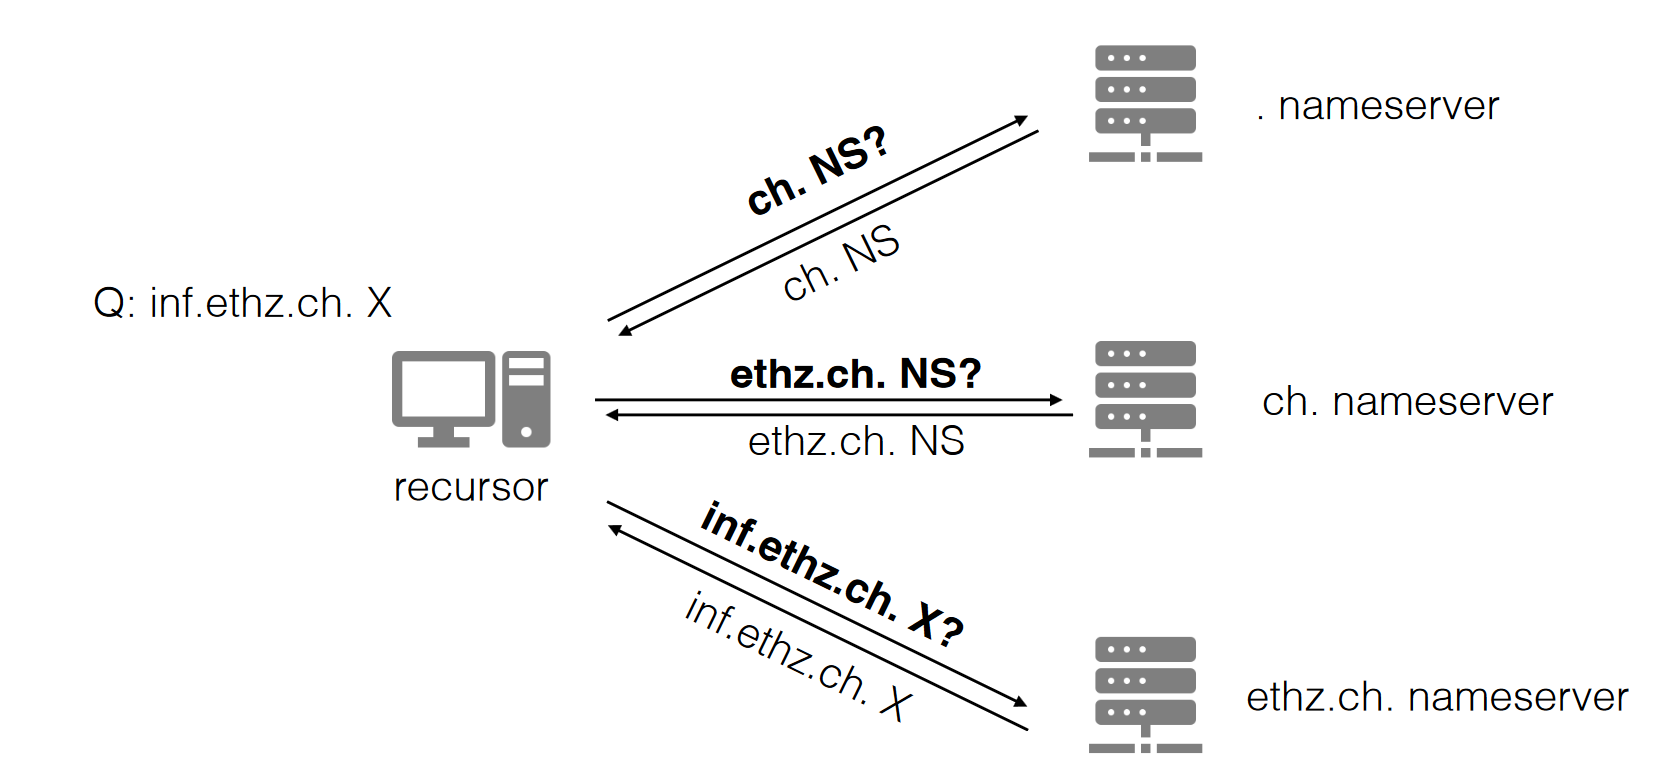
\includegraphics[width=.49\textwidth]{images/qmin.PNG}
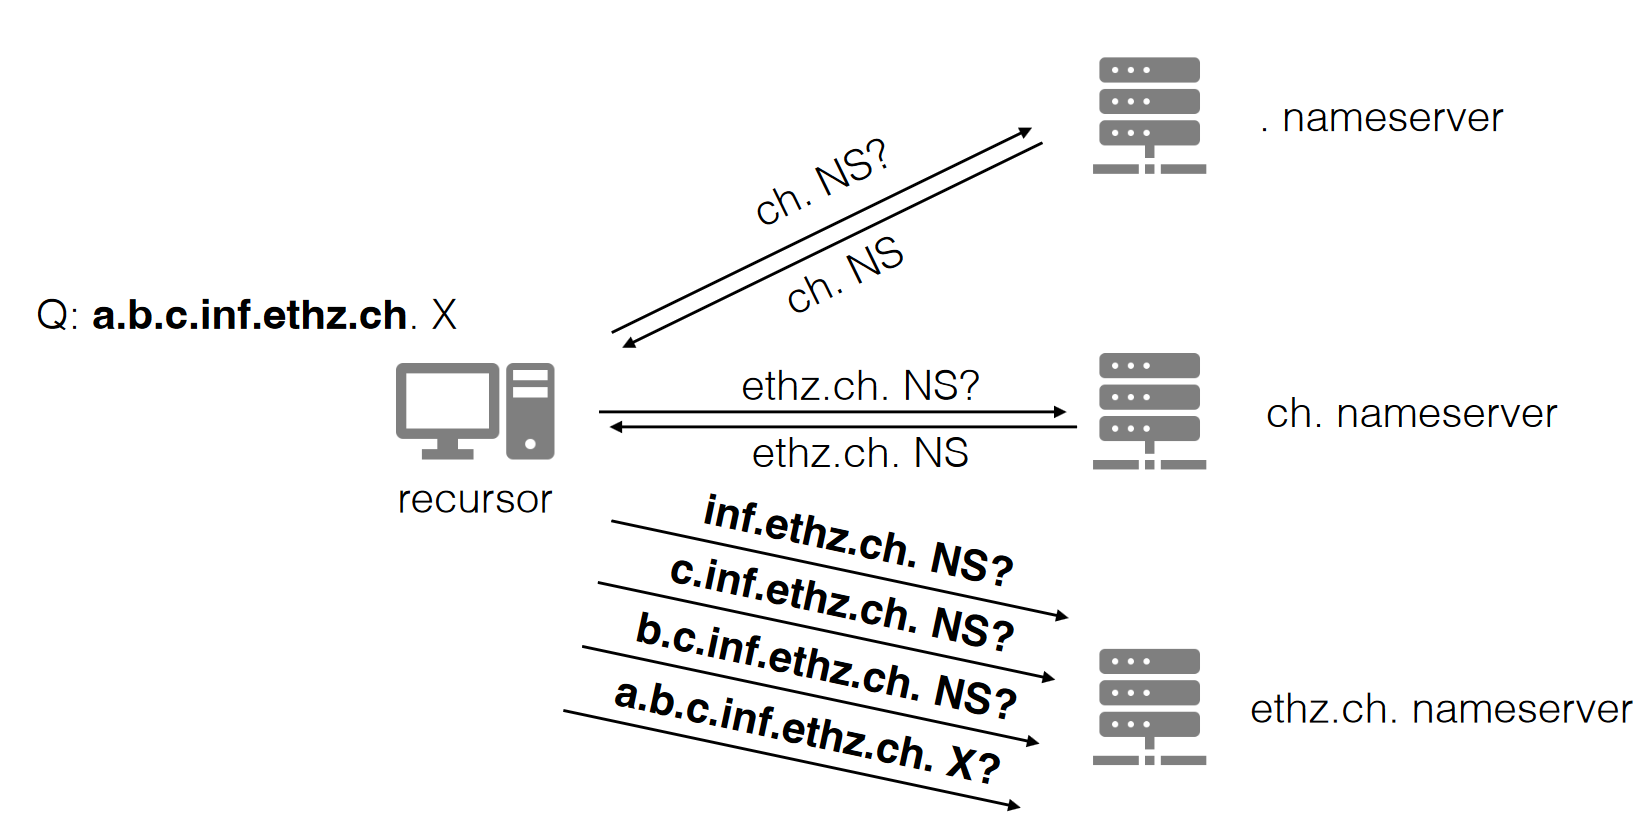
\includegraphics[width=.49\textwidth]{images/qmin_dos.PNG}
\caption{DNS Query Minimization}
\label{qmin}
\end{figure}

\subsubsection{DNS over TLS (DoT)}
DNS over TLS lets the stub resolver communicate with the recursive resolver over a TLS connection, the dedicated port for this is 853. This is supported in popular resolver implementations and enabled by popular open resolvers. To use DoT it also has to be configured in the stub resolver. An obvious issue of DoT is that it introduces the overhead of the TCP and TLS handshake. Additionally, since TCP is a stateful protocol, the stub and recursive resolver have to maintain state, which introduces new DoS attack vectors.\\
Another issue is that the trust is just relayed from the ISP to the operators of the open resolvers such as Google or Cloudflare. Furthermore, encryption disallows security monitoring of DNS traffic, which makes company policies harder to enforce. Thus, some network operators tend to block the DoT port 853.

\subsubsection{DNS over HTTPS (DoH)}
DoH encodes DNS messages in HTTP GET or PUSH messages and naturally reuses the protection from HTTPS and port 443. This approach is more browser user-friendly and gives better privacy, since the DNS traffic blends into the regular HTTPS traffic which cannot be blocked.

\subsubsection{Oblivious DNS (ODNS)}
Oblivious DNS prevents even the recursive resolver from inspecting which user sent the traffic. A client gets a new ODNS stub resolver. The following steps are used to make queries:
\begin{enumerate}
\item The stub resolver generates a session key $K$ and encrypts the domain with this key. \textit{\{foo.com\}$_k$}
\item Then the TLD \textit{.odns} is appended to the encrypted domain. \textit{\{foo.com\}$_k$.odns}
\item The session key $K$ is encrypted with the ODNS authoritative name server's public key $s$ and put into the DNS queries \textit{Additional Information} field.
\item The stub resolver sends this query to the recursive resolver.
\item The recursive resolver finds the address of the ODNS authoritative server and forwards the request to it.
\item The ODNS authoritative name server decrypts the domain using the session key $K$ and acts as a recursive resolver to resolve the query.
\item It sends back the result encrypted with the session key $K$ to the recursive resolver. \textit{Not sure about this step, didn't read the paper but it makes sense like this.}
\item The recursive resolver forwards the response back to the client.
\item The client decrypts using the session key $K$.
\end{enumerate}
Like this, the recursive resolver cannot see what the client requested and the ODNS authoritative server does not know which client the query came from since it can only see the recursive resolver.
\begin{figure}[H]
\centering
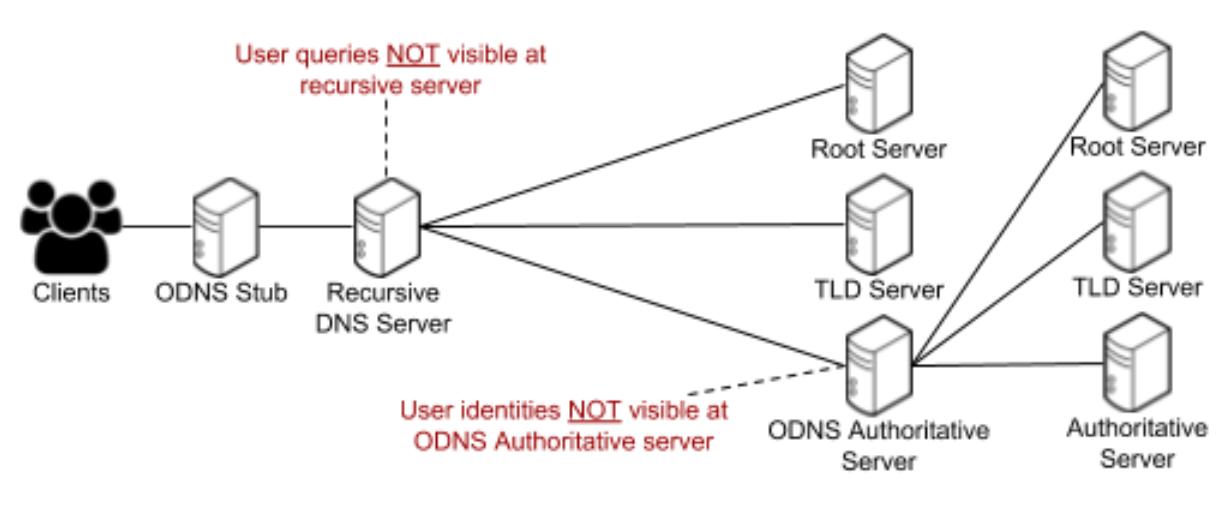
\includegraphics[width=.6\textwidth]{images/odns.PNG}
\label{odns}
\caption{Oblivious DNS}
\end{figure}

\subsection{DNS Spoofing}
An attacker may a DNS server to give back wrong information. This is done by injecting bogus records into the DNS cache, also referred to as \textbf{cache poisoning}. Since DNS does not rely on connections, the DNS server will accept the first response and ignore all subsequent responses. So in order to inject a record into the cache, the forged response has to arrive before the real one. Further, the response has to match the query, meaning that destination/source IP addresses and destination/source port numbers as well as the txid query identifier have to match. We'll look at what the attacker has to do in certain situations.

\subsubsection{On-Path Eavesdropper}
This case is by far the easiest. Since DNS traffic is unencrypted, the attacker can simply eavesdrop on the query, read out all the parameters and forge a response. Since the attacker does not have to do a lot of processing, the attacker will be faster than the legitimate server in most cases. To be more certain, the attacker could also start put a lot of load on the legitimate name server, such that the processing of the request will be slower.

\subsubsection{Malicious Auth Server}
In early DNS, tehre was a flaw that all the data in the additional section of the response is unrestricted and cached. This means that a legitimate name server could essentially write any records into the cache of the recursive resolver by simply including those records in the additional section. This was possible, even when the additional data did not match what was transmitted in the authority server, i.e. the name server did not have authority over. This led resolvers to not accept and cache additional records that were not within the authority zone of that server.

\subsubsection{Off-Path Attacker}
If the attacker is not on the path, he has no way to figure out the parameters of the query. Since DNS was operated on standard ports and the IP addresses are obvious as well, the main issue was the 16-bit random txid query identifier. In each race, the attacker had to guess among 65536 possible txids and if he lost the race, the legitimate answer would be cached and the attacker would have to wait for the TTL to expire.\vspace{.3cm}\\

The infamous \textbf{Kaminsky attack} found a way to bypass the cache and also pass the checking of additional data. The attacker would trigger many queries for subdomains in parallel. Then it would flood the resolver with many referral replies containing a random txid. In those replies, the attacker pretends to be the legitimate server returning an NS record as well as a glue record in the additional section that contains the malicious IP. Since the content in the additional section lies within the authority zone of that server, the content is accepted and cached. This attacking strategy put almost every name server on the planet at risk and caused unprecedented attention to DNS security. To prevent such attacks, source port randomization was enforced, enlarging the search space for the attacker from $2^{16}$ to $2^{32}$.\vspace{.3cm}\\

The \textbf{SADDNS} attack again found a way around this. It exploits that the resolver opens a source port once it receives a query. The attacker launches a query and uses a port scan to check which port is open. If the port is closed, the resolver will reply with an ICMP port unreachable message. Once the open source port has been found, the rest is just Kaminsky.


\section{SCION}
SCION stands for \textit{A Secure Multipath Interdomain Routing Architecture}. The current Internet's design has many shortcomings and lacks communication guarantees. It is susceptible to a variety of different attacks and outages occur regularly. The current Internet also suffers from several \textit{kill switches} that can halt communication within a geographical area and therefore rupture sovereignty. As the Internet has grown to encompass a large part of the global population, trust relationships have become heterogeneous, no single entity is trusted by everyone. This complicates the construction of entity authentication infrastructures. Current authentication infrastructures have weak security properties. \vspace{.3cm}\\

One protocol that causes a lot of issues is BGP and BGPsec. It fundamentally limits the availability, transparency, control, and trust that could be possible in the Internet. Due to its slow convergence during the iterative route computation, destinations are frequently unavailable. It is susceptible to attacks and misconfiguration that sometimes result in global outages. Furthermore, paths are hard to predict and reproduce, end points have almost not choice over how their traffic flows, and the trust is centred in very few trust roots, which represent single points of failure.

SCION is the result of the question: How good could the Internet be if we started from scratch? Here are a few of SCION's architecture principles:
\begin{itemize}
\item Stateless packet forwarding (no inconsistent forwarding state)
\item \textit{Instant convergence} routing
\item Path-aware networking
\item Multi-path communication
\item High security through design and formal verification
\item Sovereignty and transparency for trust roots
\end{itemize}
\begin{figure}[H]
\centering
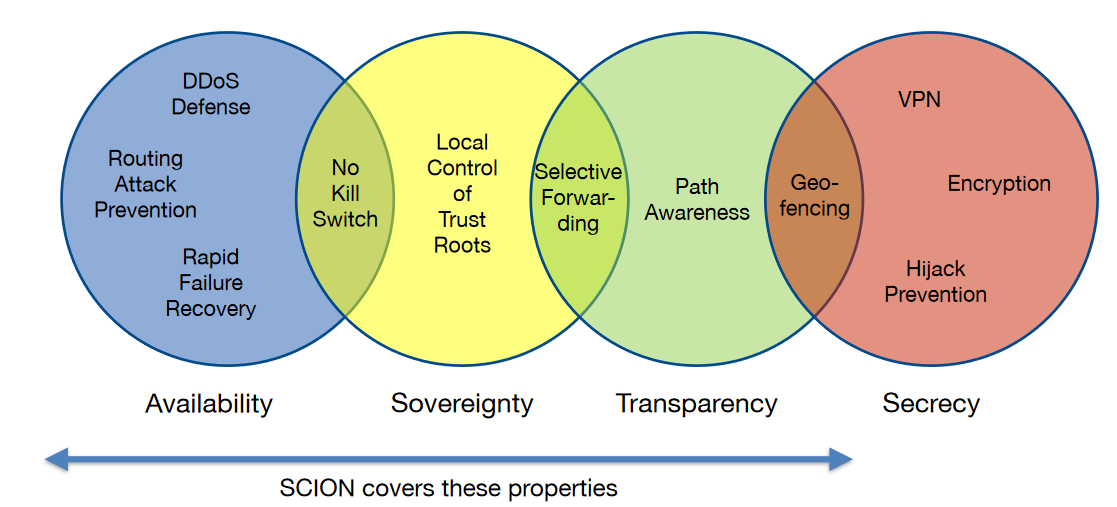
\includegraphics[width=.7\textwidth]{images/scion_properties.PNG}
\label{scion_properties}
\caption{SCION Properties}
\end{figure}

\subsection{Control Plane}
The control plane of an inter-domain routing protocol is responsible for finding end-to-end paths between autonomous systems. SCION does this by implementing \textbf{path exploration} and \textbf{path registration}. First, we look at how SCION approaches the scalability of their network. The autonomous systems are grouped into so-called \textbf{isolation domains (ISD)}, the autonomous systems in an isolation domain agree on their trusted roots. A group of \textbf{core ASs} forms the \textbf{IDS core}, which manages the ISD. The control plain is organized hierarchically into an inter-ISD and intra-ISD control plane. Furthermore, each ISD defines their \textbf{trust root configuration (TRC)} which contains the root cryptographic keys to verify ISD operations. 
\begin{figure}[H]
\centering
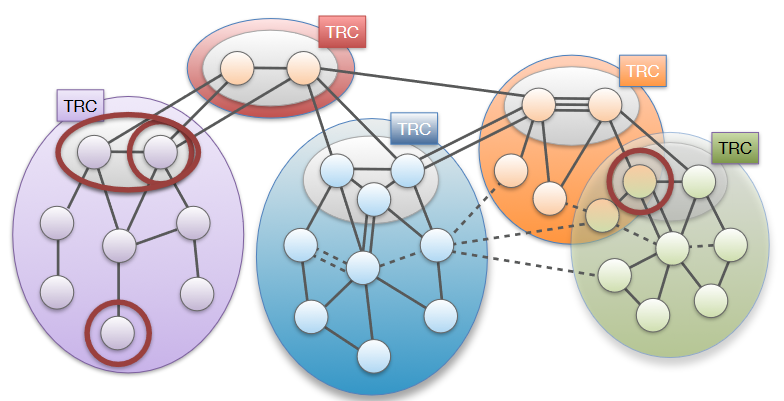
\includegraphics[width=.6\textwidth]{images/control_plane.PNG}
\caption{Isolation Domains}
\label{control_plane}
\end{figure}

Paths inside the ISD are found using \textbf{beaconing}. The core ASs initiate \textbf{Path-segment Construction Beacons (PCBs)}. These PCBs traverse the ISD as a flood to reach downstream ASs. Each AS receives multiple PCBs representing path segments to a core AS. To implement this, each AS deploys one or multiple beacon servers. The PCBs are sent out via a SCION service anycast packet and reach a border router of the AS, which then select one beacon server and forward the PCB to it. The beacon servers coordinate to resend the PCBs periodically to downstream ASes. Currently every hour or on change, PCBs are selected and forwarded.\\
A PCB contains an information field with the PCB creation time. Each AS on the path adds the following:
\begin{itemize}
\item AS name
\item Hop field for data-plane forwarding
\begin{itemize}
\item Link Identifiers
\item Expiration Time
\item Message Authentication Code (MAC) 
\end{itemize}
\item AS signature
\end{itemize}
\begin{figure}[h]
\centering
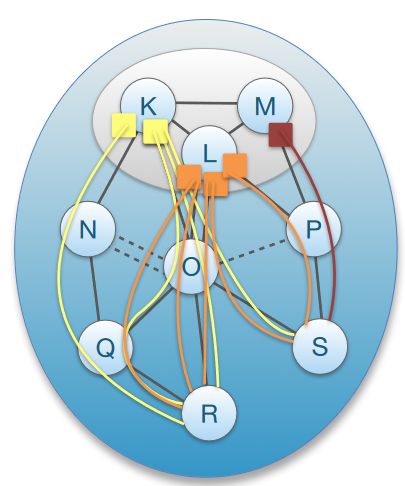
\includegraphics[width=.4\textwidth]{images/isd_path.PNG}
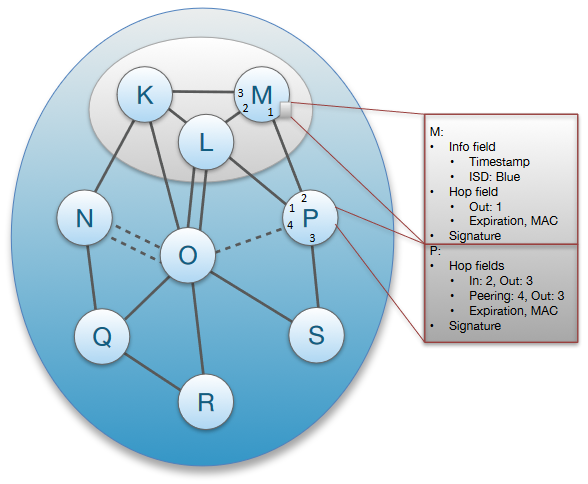
\includegraphics[width=.5\textwidth]{images/beaconing.PNG}
\label{beaconing}
\caption{Path-Segment Construction Beacons}
\end{figure}
These path segments are reversible, meaning they can act as both up-path segments from AS to core AS or as a down-path segment from core AS to AS.\\
Inter-ISD path exploration works basically the same. Each core AS sends out those beacons to construct path-segments to all other isolation domains. This is similar to BGP since the core ASs of every isolation domain construct paths between each other. However, since the number of isolation domains is reasonably small, this \textbf{core beaconing} is still scalable.\vspace{.3cm}\\

These path-segments are then provided via the \textbf{path server infrastructure}. The path servers offer a lookup service, similar to DNS. The core ASs operate core path servers, which store consistent down-path segments and core-path segments. Each non-core AS runs a local path server that serves up-path segments to the local clients, resolves and caches response of remote AS lookups.\\
Which paths are registered is decided by the AS. The AS can look at all path-segments it received via PCBs and decide which of those it wants to use as up-paths. These path-segments then get registered at the local path server. Path-segments that are deemed acceptable as down-paths are registered at the core path servers. This allows for ingress path control, i.e. the AS itself defines how others get to it.

\subsection{Data Plane}
If a host wants to send a packet, it first has to lookup a path to the destination. For this it contacts a \textbf{RHINE} server, which provides similar functionality to a DNS server. The host sends a query containing a domain and the RHINE server responds with the ISD number, the AS number and the local address at the destination. The host then contacts the local path server to query the path segments. The path server responds with an up-path, core-path and down-path segments. The host combines these path segments to obtain end-to-end paths, which are added to the packers.\\
If the local path server does not have the information cached, it sends a request to the core path server. If the core path server does not have the path segments cached, it will contact a remote core path server. Once all the path segments are received, they can be combined in various ways. For example, if up- and down-path segments both offer the same peering link, a peering shortcut can be taken, or if both segments share a common AS, the combined path does not have to go all the way to the core.\vspace{.3cm}\\

Because the actual local address is not needed for routing until the destination AS, the SCION packet header supports various addressing modes. This goes so far that the source and destination could even have the same local address, or the source address being IPv4 and the destination address being IPv6.
The header also includes version numbers, address types, and path information with pointers to the current info and hop field, as well as a next header field. The local addresses are at a fixed location and padded if necessary.\\
\iffalse
TODO
- MTU discovery
- NDP
- hierarchical routing
\fi
\end{document}